\chapter{MOTION PRIMITIVE TWEAKING:BIPEDAL WALKING}
\label{chap:walk}

\ifpdf
    \graphicspath{{BipedWalk/BipedWalkFigs/PNG/}{BipedWalk/BipedWalkFigs/PDF/}{BipedWalk/BipedWalkFigs/}}
\else
    \graphicspath{{BipedWalk/BipedWalkFigs/EPS/}{BipedWalk/BipedWalkFigs/}}
\fi

In previous chapters, bouncing ball and mass spring are only used for illustrate the theory, but have little value for graphic application and motor control research.
In this chapter, we will discuss in details about how to adaptive motion primitve for for different environment and met user's needs.
How motion primitives connected will be discussed in the next chapter.


The motion primitive we use is bipdeal walking.
bipedal walking is a topic of great application value for both the graphic and robotic engineering.
Currently, it is special ability robtos can't compete with human.

In the past a few decades, almost all the control method have been tried on the bipedal walking model, but still we don't achieve the human bipdeal walking ability.
At the begining, researchers believe bipedal walking in nature is unstable, and developped lots of control method based on trajectory following.
A great turning point is the discovery of passive dynamic walking machine, it shows walking can happens without any control effort.
This idea lead us to believe that walking is an inborn ability, and most problem are solved our body mechanical structure.

In our research, we took the passive walking gait as motion primitive, we use global and local motor invariant controller to boot stability and adaptation.
By this method ,we get rid of solving complex computational burden.
We generate adaptive and natural looking gait in a computational efficient way.


\section{Motion Primitives}


For bipedal walking, the main motion happens in the spagittal plane.
as shown in figure
\begin{figure}[!htbp]
  \begin{center}
      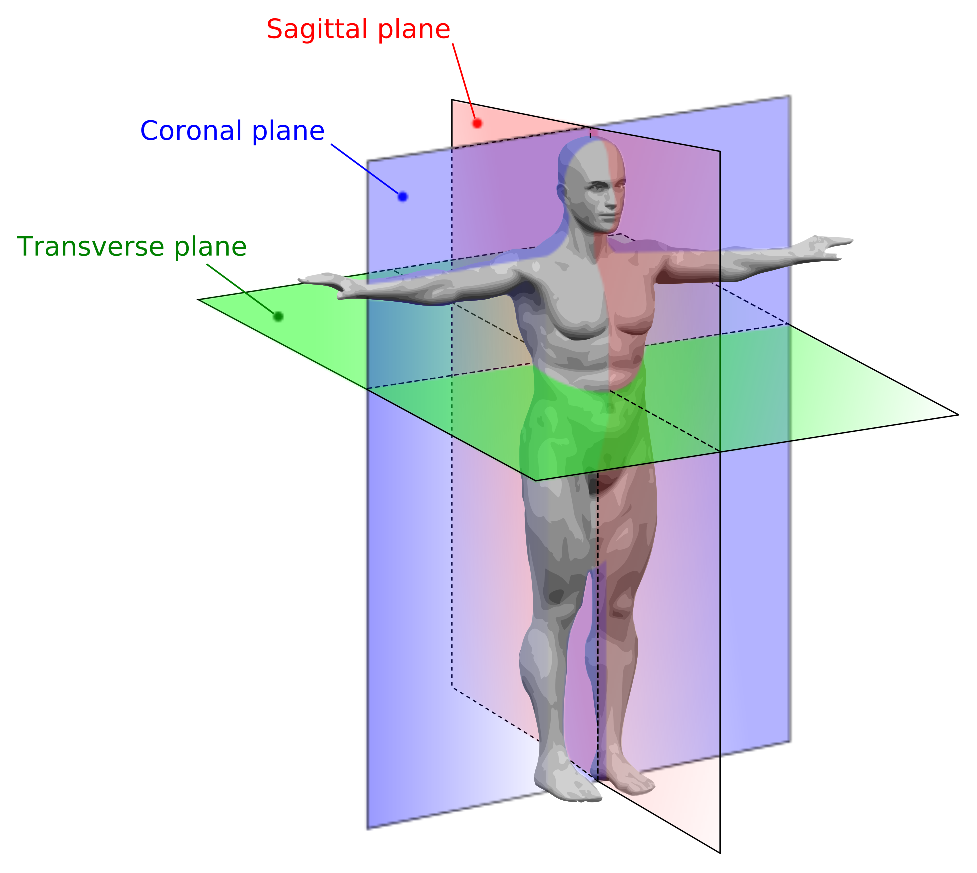
\includegraphics[width=0.7\textwidth]{spahittalPlae}
    \caption{SpahittaPlane}
    \label{fig:passivekneewalker}
\end{center}
\end{figure}



Sidesway and row motion are relative small and usually treated as secondary motion or totally neglected.
In this chapter, we mainly focus on the two dimension motion, which captured most of key characterstics of motion, and maintain the completeness of our theory.
For motion of more dofs, are discussed in Chapter 8, the effects of more dofs will introduce perturbation to our model, they will not change the basic motion characteris and adaptation tendency.
But they will made the ''symmetry'' not so perfect, and may cause confusion.
Thus we wil delay the discussion of fullbody in later chapter.

\begin{figure}[!htbp]
  \begin{center}
      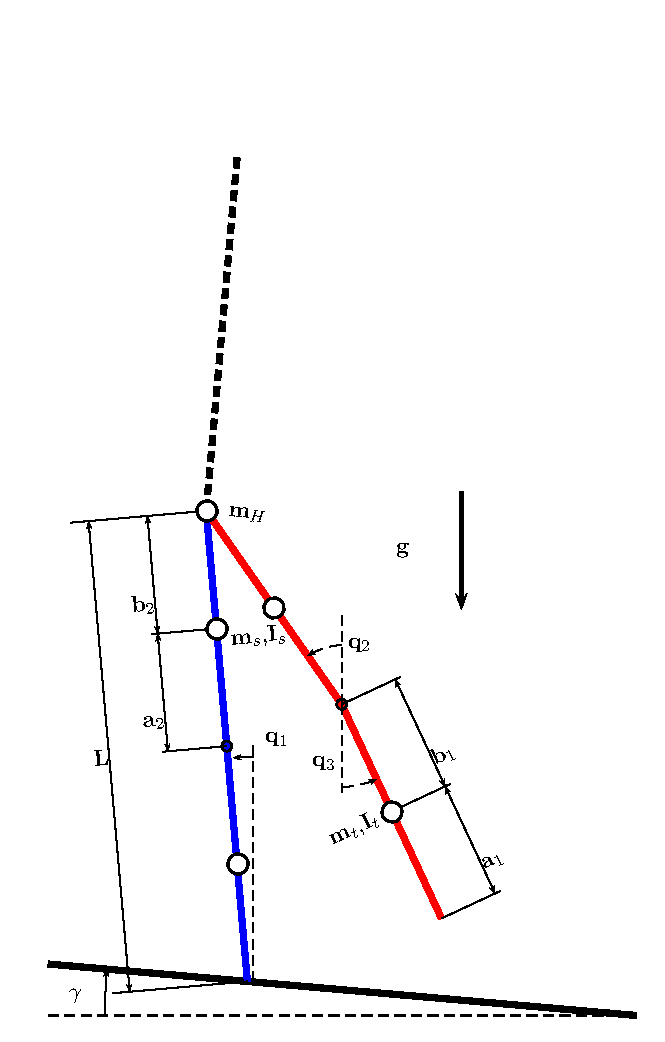
\includegraphics[width=0.7\textwidth]{PWI}
    \caption{A Passive Walking Model with Knee}
    \label{fig:passivekneewalker}
\end{center}
\end{figure}


Figure~\ref{fig:passivekneewalker} shows the a two dimensional walking model.
\subsection*{Dynamics}
If put on a downslope, with some special initial condition, the passive walker can walking down the slope with a stable gait.
On the phase plot, we will have a limit circle Figure ~\ref{fig:fourphaselimitcycle}.
Like bouncing ball, this system is also an hybrid system,the motion include four phases\citep{Chen2007}.
\begin{itemize}
\HiItem{Free Swing Phase}
During this phase, the support leg (the blue one) is kept straight and there is no knee bending with the supporting leg.
The Swing Leg is bended, the thigh and shank.
\HiItem{Knee Strike Phase}
The Knee Joints has a limit, we suppose when the knee angle reach the limit,a collision happens,after that the swing leg is kept straight.
\HiItem{Knee Lock Swing Phase}
During this phase, both the swing and support leg are kept straight.
\HiItem{Heel Strike Phase}
When Heel Collid with the ground, heel strike happens and switch the stancing and swaying leg.
\end{itemize}

\begin{figure}[!htbp]
  \begin{center}
    \leavevmode
    \ifpdf
      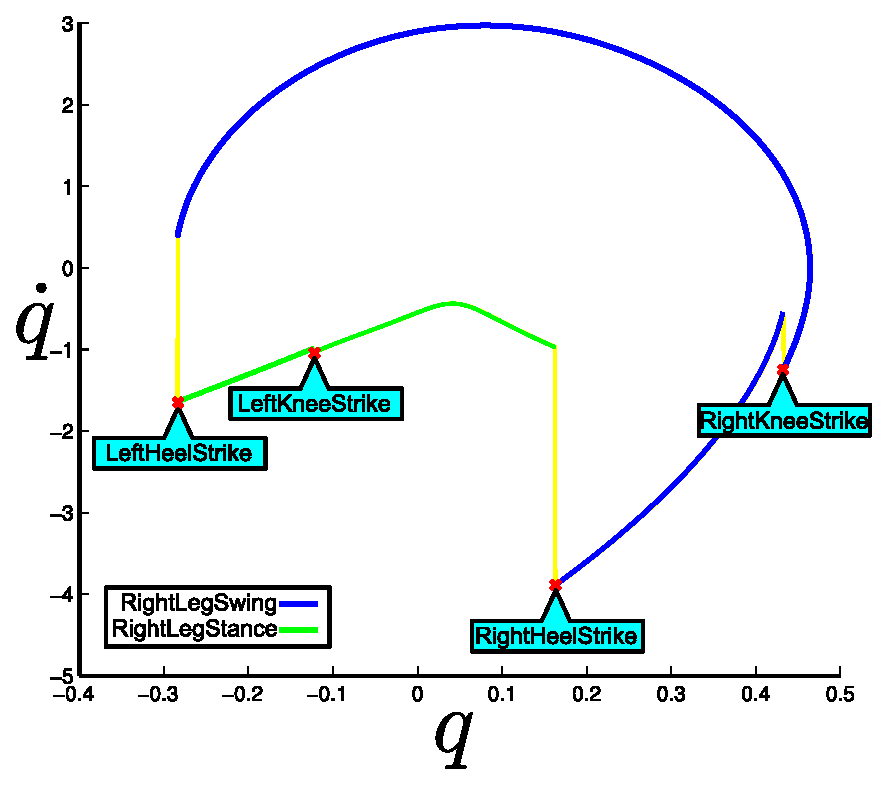
\includegraphics[height=6in]{walk_cycle_index}
    \else
      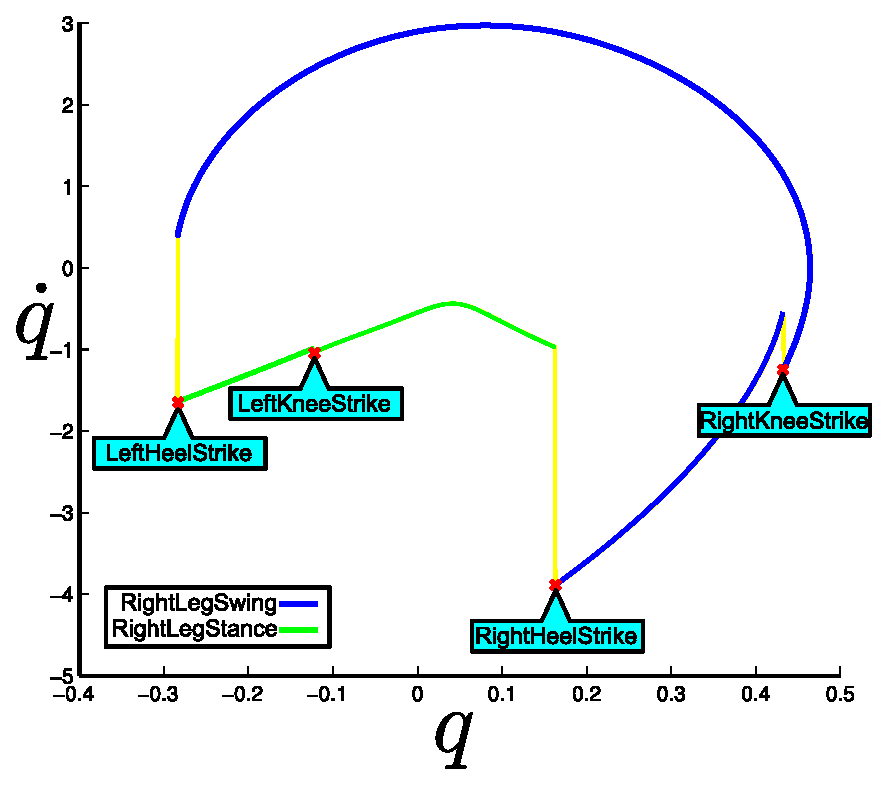
\includegraphics[width=0.7\textwidth]{walk_cycle_index}
    \fi
    \caption{Limit Circle And Different Phase in Passive Walking}
    \label{fig:fourphaselimitcycle}
\end{center}
\end{figure}


\begin{figure}[!htbp]
  \begin{center}
    \leavevmode
    \ifpdf
      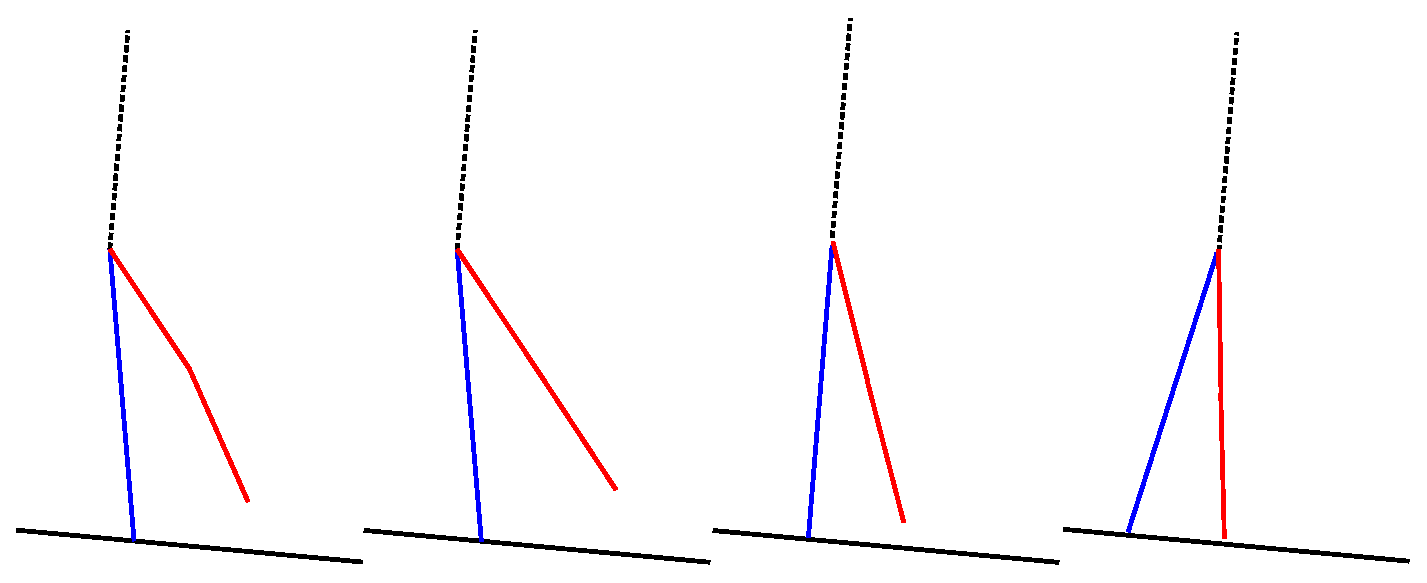
\includegraphics[height=6in]{Fourphase}
    \else
      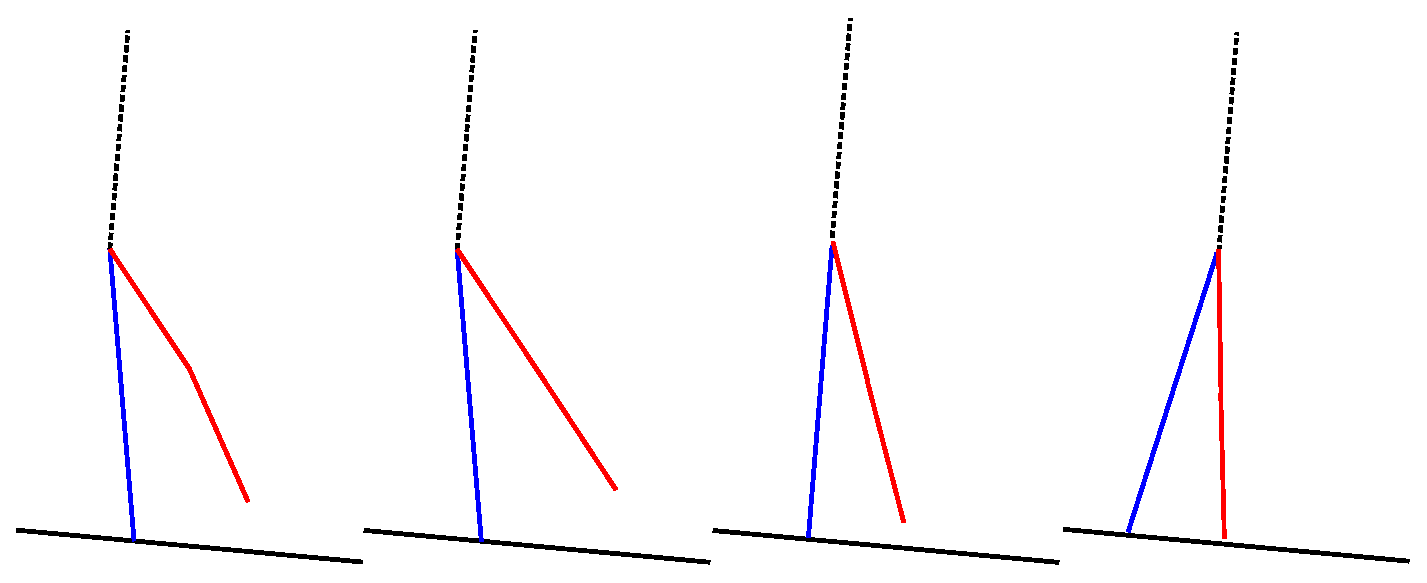
\includegraphics[width=0.7\textwidth]{Fourphase}
    \fi
    \caption{The four phases in Walking}
    \label{fig:fwalkingphase}
\end{center}
\end{figure}

\subsubsection*{Dynamic Equation}

The passive walking are modelled as rigid body dynamics.
for details of caculating the dynamic equation, please reference\citep{Chen2007}
The Passive Walking equation is developed based on Lagrange Mechanics.


\begin{itemize}
\HiItem{flying phase}
the equation are in the form of 
\begin{equation}
\label{eq:flyequation}
M(\mathbf{q}) \ddot{\mathbf{q}} + C(\mathbf{q,\qd})\dot{\mathbf{q}} + N(\mathbf{q}) = 0
\end{equation}
$q=[q_1,q_2,q_3]$,$\qd=[\dot{q_1},\dot{q_2},\dot{q_3}]$
where $M$ is the initial mass matrix, $C$ and $N$ are the centrifugal force matrix and gravity respectively. The knee lock and contact state applies the instantaneous function
for knee free a  $M$ and $C$ are 3 by 3 Matrix, $N$ is 3 by 1 matrix.
for knee lock phase, $M$ and $C$ are 2 by 2 Matrix, $N$ is 2 by 1 Matrix.


Equation ~\ref{eq:flyequation} can also in the state form, we have $\state=[q,\qd]$.
Then the function is in the form.
\begin{equation}
\dot{\state}=
-\left[ 
\begin{array}{cc}
\mathbf{1} &0\\
0 &M 
\end{array}
\right]^{-1}
\left[ 
\begin{array}{cc}
0 &\mathbf{1}\\
0 &C 
\end{array}
\right]\state
-\left[ 
\begin{array}{c}
\mathbf{0}\\
 N 
\end{array}
\right]
\end{equation}

\HiItem{The Strike Phases}
When Heel Strike or Knee Strike Happens.
collision equations are developed by momentum perserving laws.
for the two phase, equations are off the same form.
\begin{equation}
Q^{+}\dot{\mathbf{q}}^{+} = Q^{-}\dot{\mathbf{q}}^{-}
\end{equation}
where $Q$ is the mass matrix used to compute the angular momentum inetia, before and after a heel strike or knee lock
For Knees Strike,$Q^-$ is 3 by 2 Matrix, $Q^+$ is 2 by 2 Matrix;
For Heel Strike, both $Q^{+,-}$ are 2 by 2 Matrix.
\end{itemize}
For the commponents of each matrix, please refer to the appendex.




\section{Global Motor Control And Adaptive Gaits}

\subsection{Entrainment}

When Coupling Neural Oscillator with the Passive Walker,
the output of neural oscillator drive the hip angel(angle between the two thighs)
as shown in equation
\begin{equation}
M(\mathbf{q}) \ddot{\mathbf{q}} + C(\mathbf{q,\qd})\dot{\mathbf{q}} + N(\mathbf{q}) = D\uout
\end{equation}
for the knee lock phase $D=[1,1]^T$.
for knee free phase, $D=[1,-1,0]^T$(acting on the difference between the two thighs, not effect the knee)

the input signal is the hip angle,
we have 
\[
	\uin=\hin(q_1-q_2)
\]

when the drive force is small, the entrainment system show a similar limit circle with original passive one,
thus result in a similar gait.
limit circle and gait are show in figure and figure 

\begin{figure}[!htbp]
  \begin{center}
    \leavevmode
    \ifpdf
      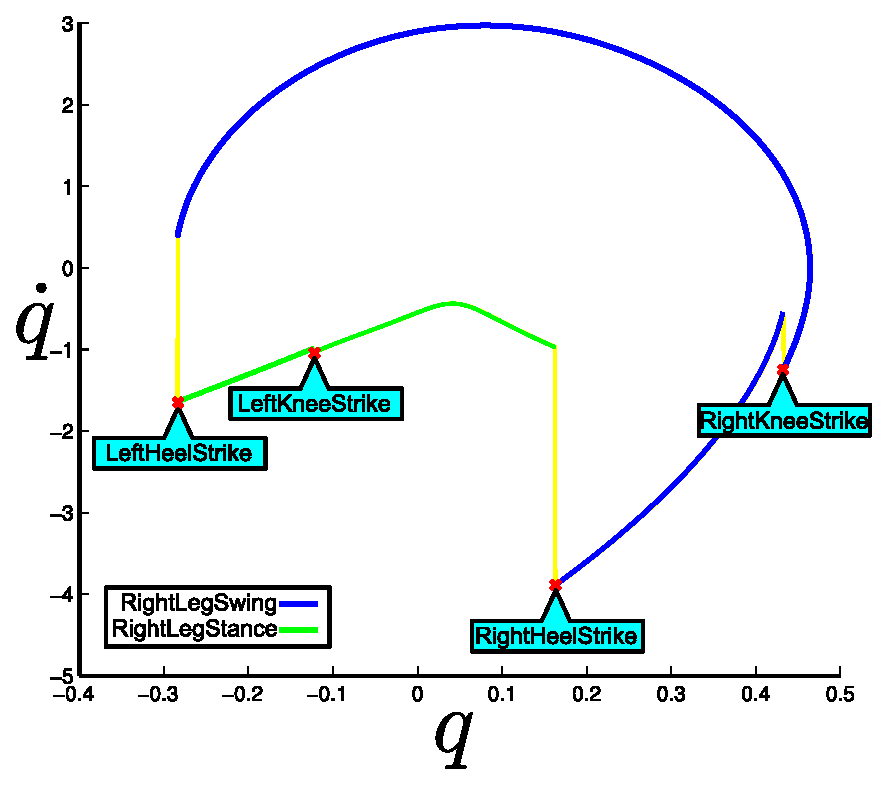
\includegraphics[height=6in]{walk_cycle_index}
    \else
      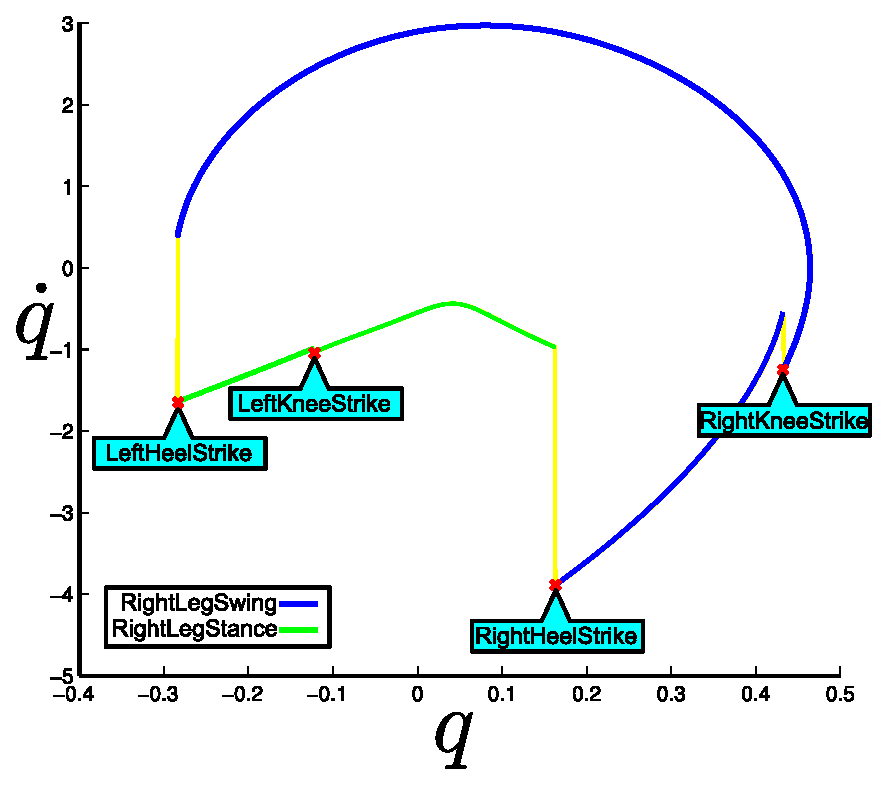
\includegraphics[width=0.7\textwidth]{walk_cycle_index}
    \fi
    \caption{Place Holder}
    \label{fig:Passive And Entraintment Walking Comparation}
\end{center}
\end{figure}

\begin{figure}[!htbp]
  \begin{center}
    \leavevmode
    \ifpdf
      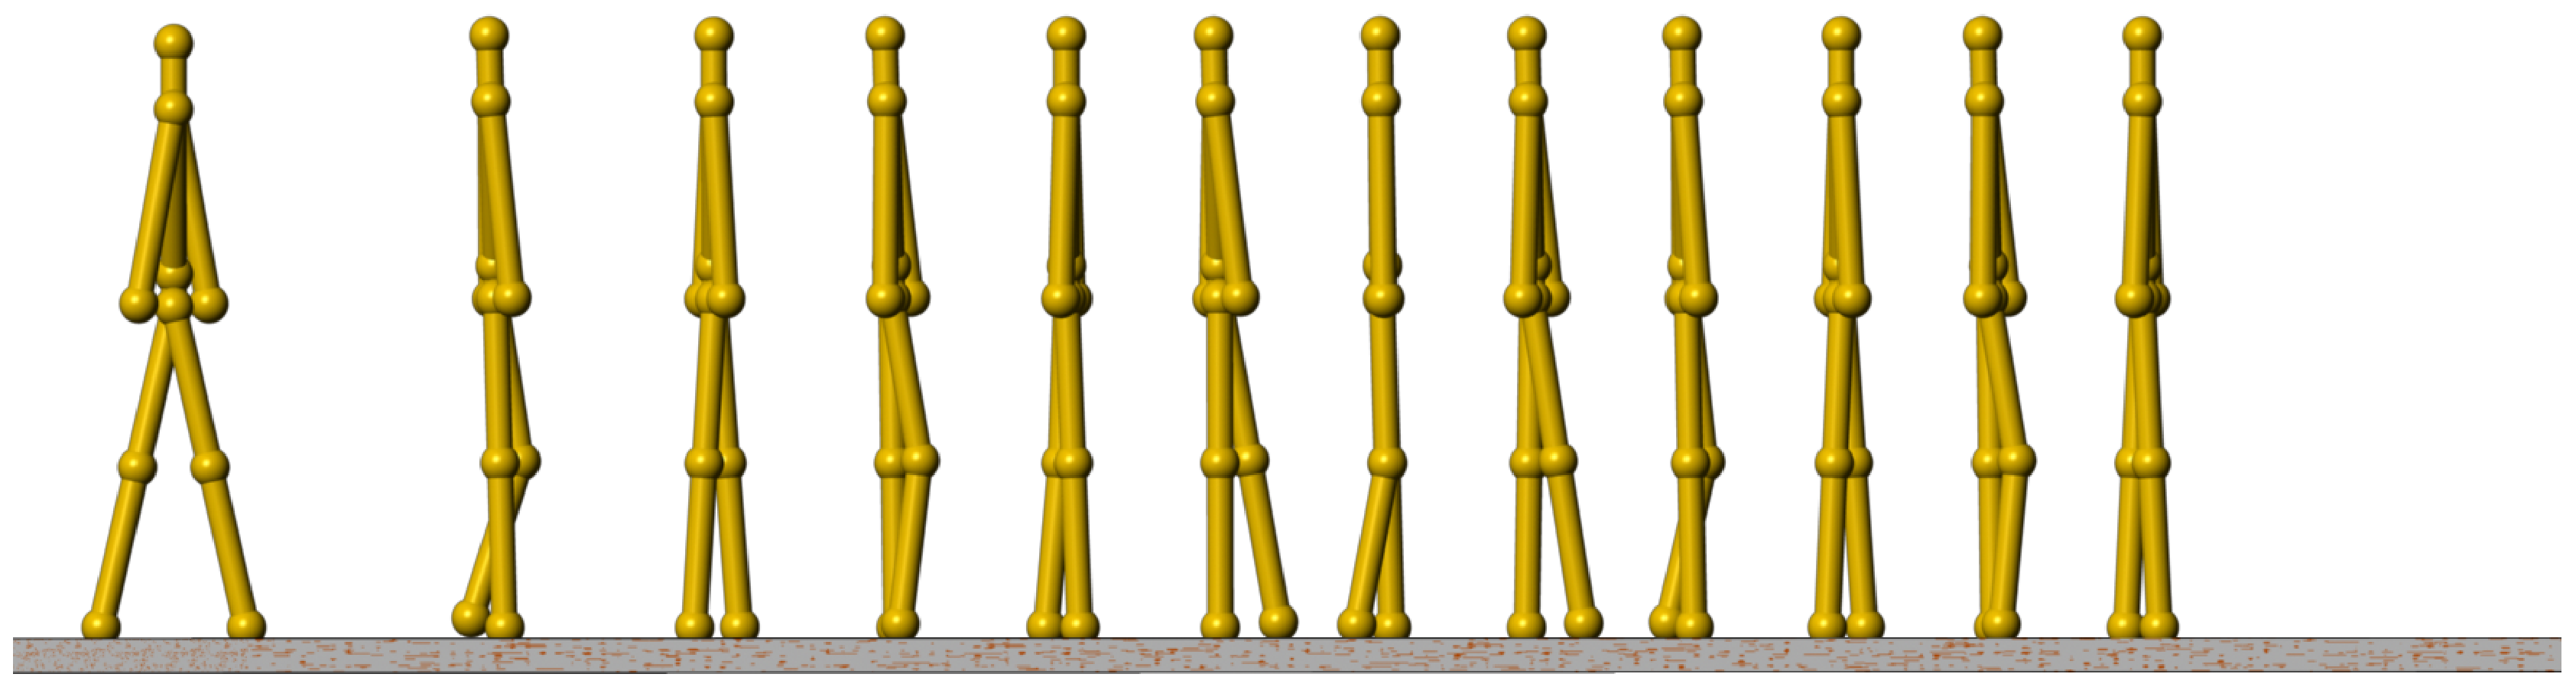
\includegraphics[height=6in]{walking_with_neural}
    \else
      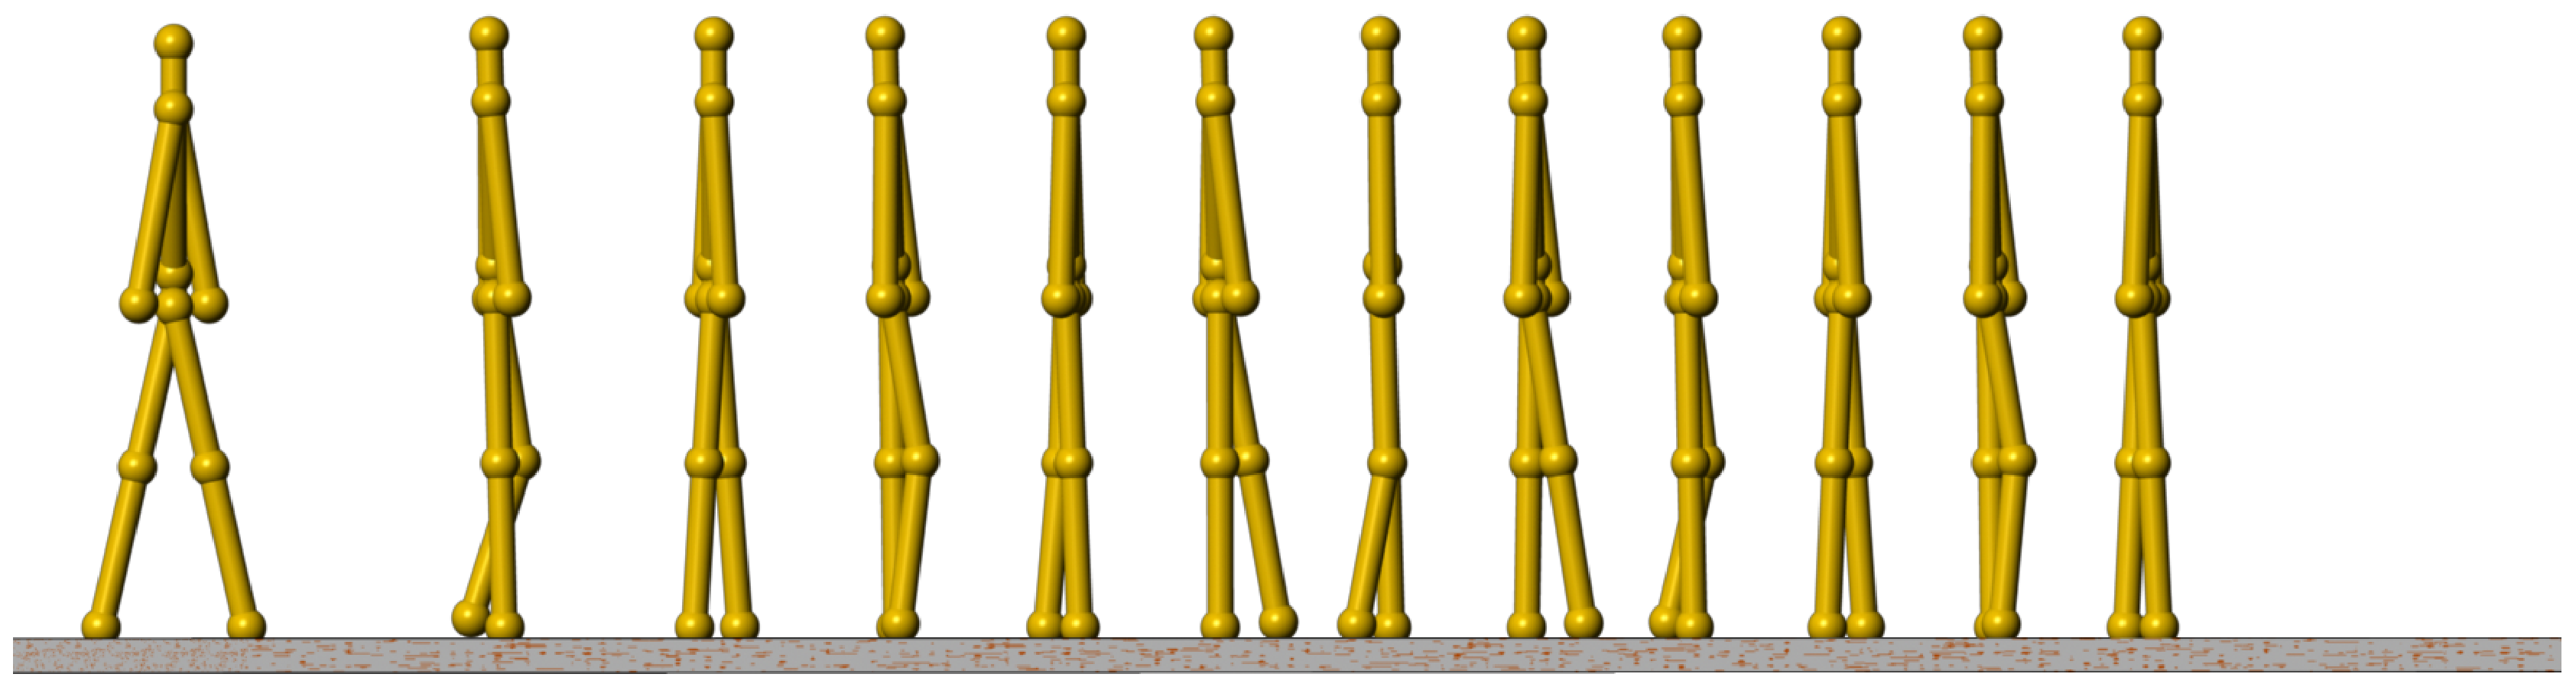
\includegraphics[width=0.7\textwidth]{walking_with_neural}
    \fi
    \caption{Place Holder}
    \label{fig:passivegait}
\end{center}
\end{figure}

\begin{figure}[!htbp]
  \begin{center}
    \leavevmode
    \ifpdf
      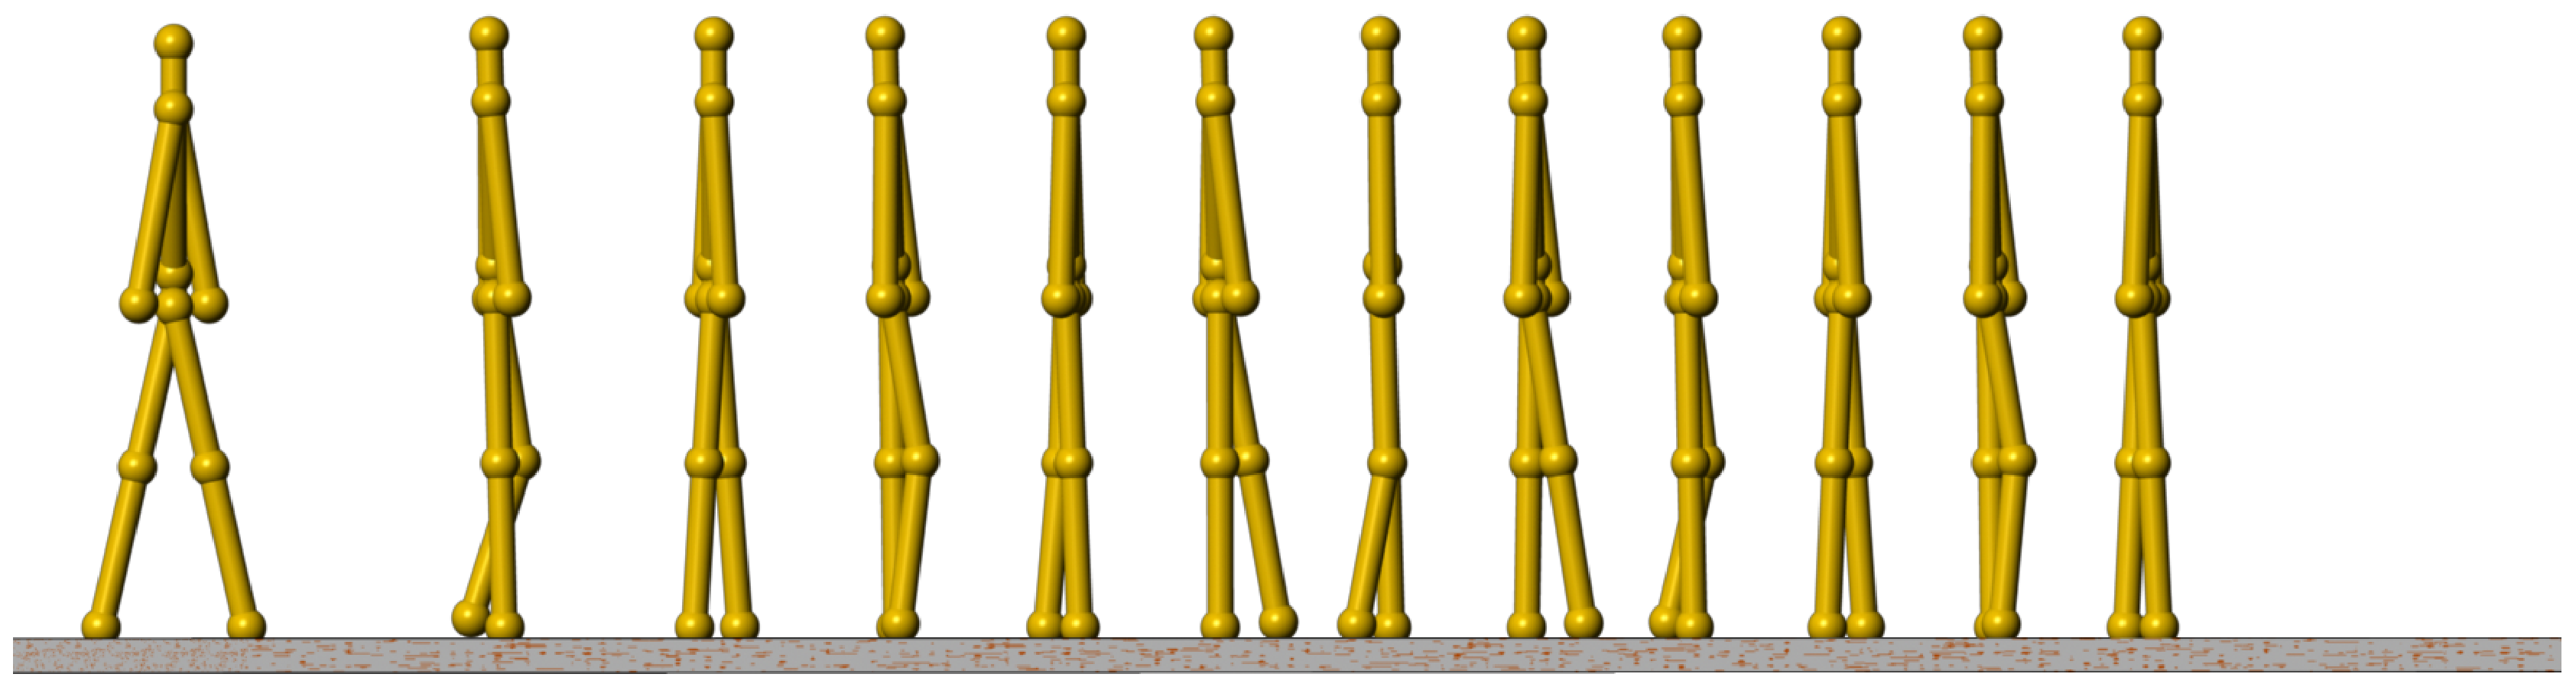
\includegraphics[height=6in]{walking_with_neural}
    \else
      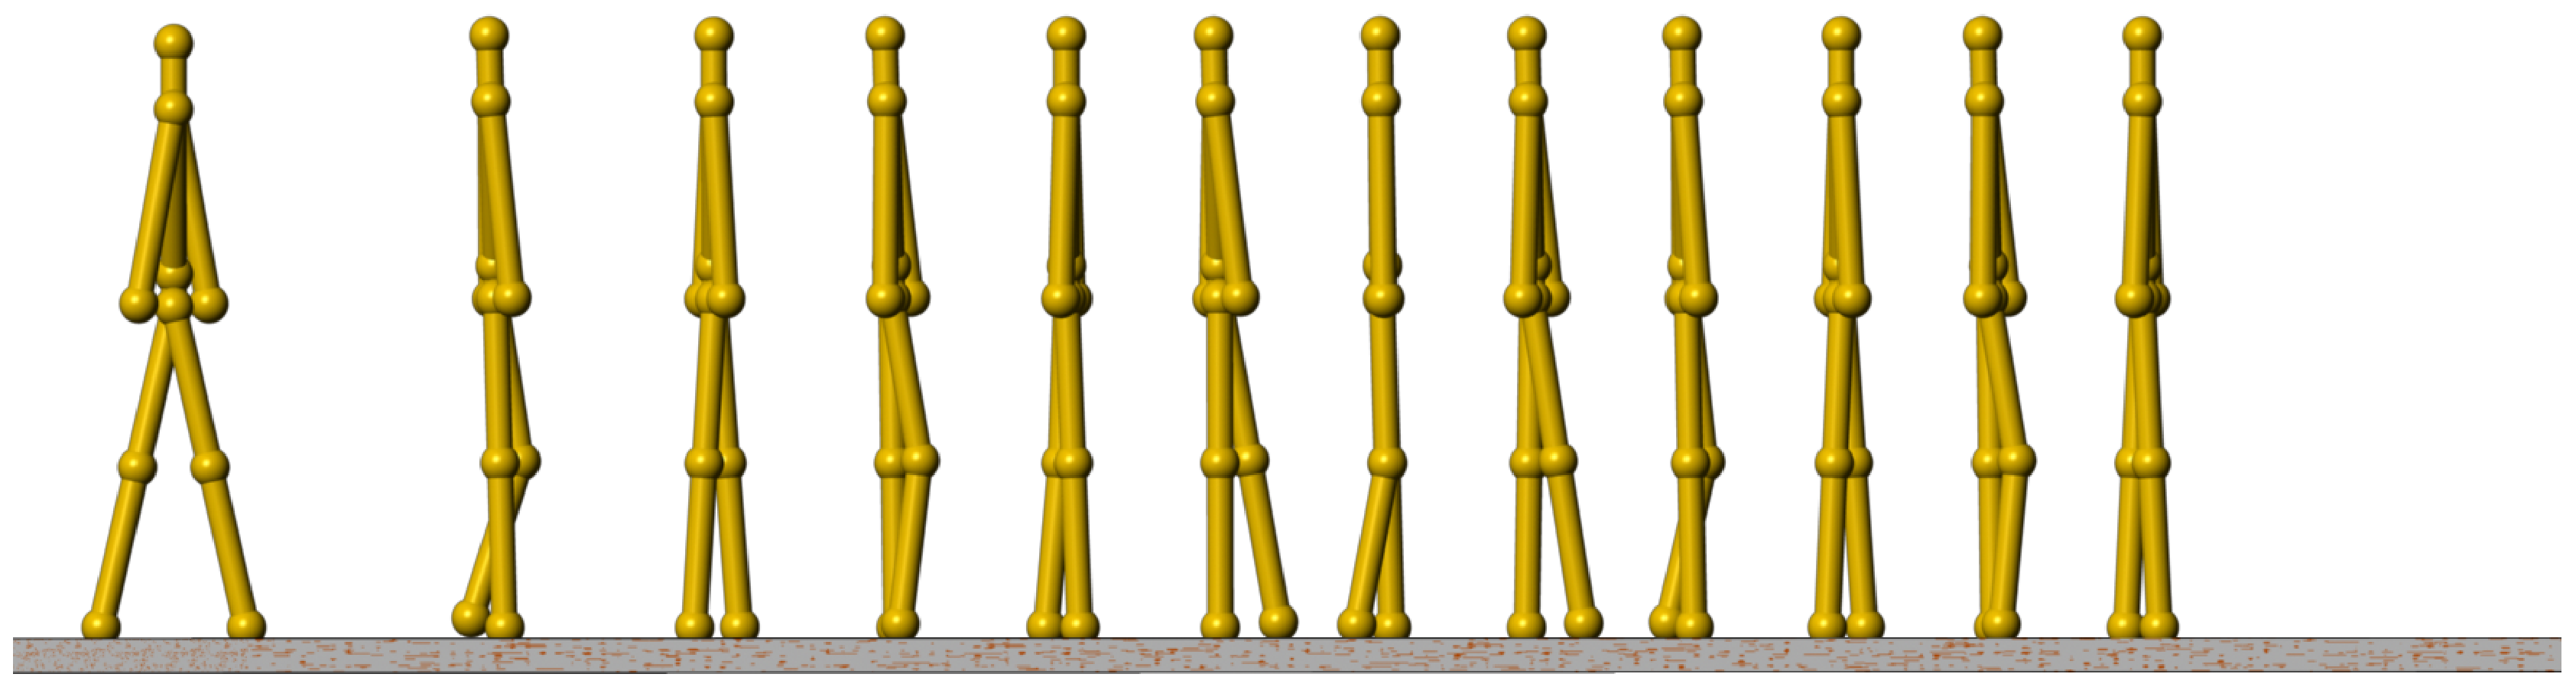
\includegraphics[width=0.7\textwidth]{walking_with_neural}
    \fi
    \caption{Place Holder}
    \label{fig:entrainmentgait}
\end{center}
\end{figure}



Entrainment Boost the staliby of the passive dynamic walker, 
the original walker can't walk on plain, when after several steps, the step size will become smaller and finally will rest or fall over.
after coupline with neural oscillator, the passive walker can walk on a plane with constant stepsize.
To main the energy efficient proper of natural motion, we make the limit the $\hout$ to a small numer, thus the step size is very small.

\begin{figure}[!htbp]
  \begin{center}
    \leavevmode
    \ifpdf
      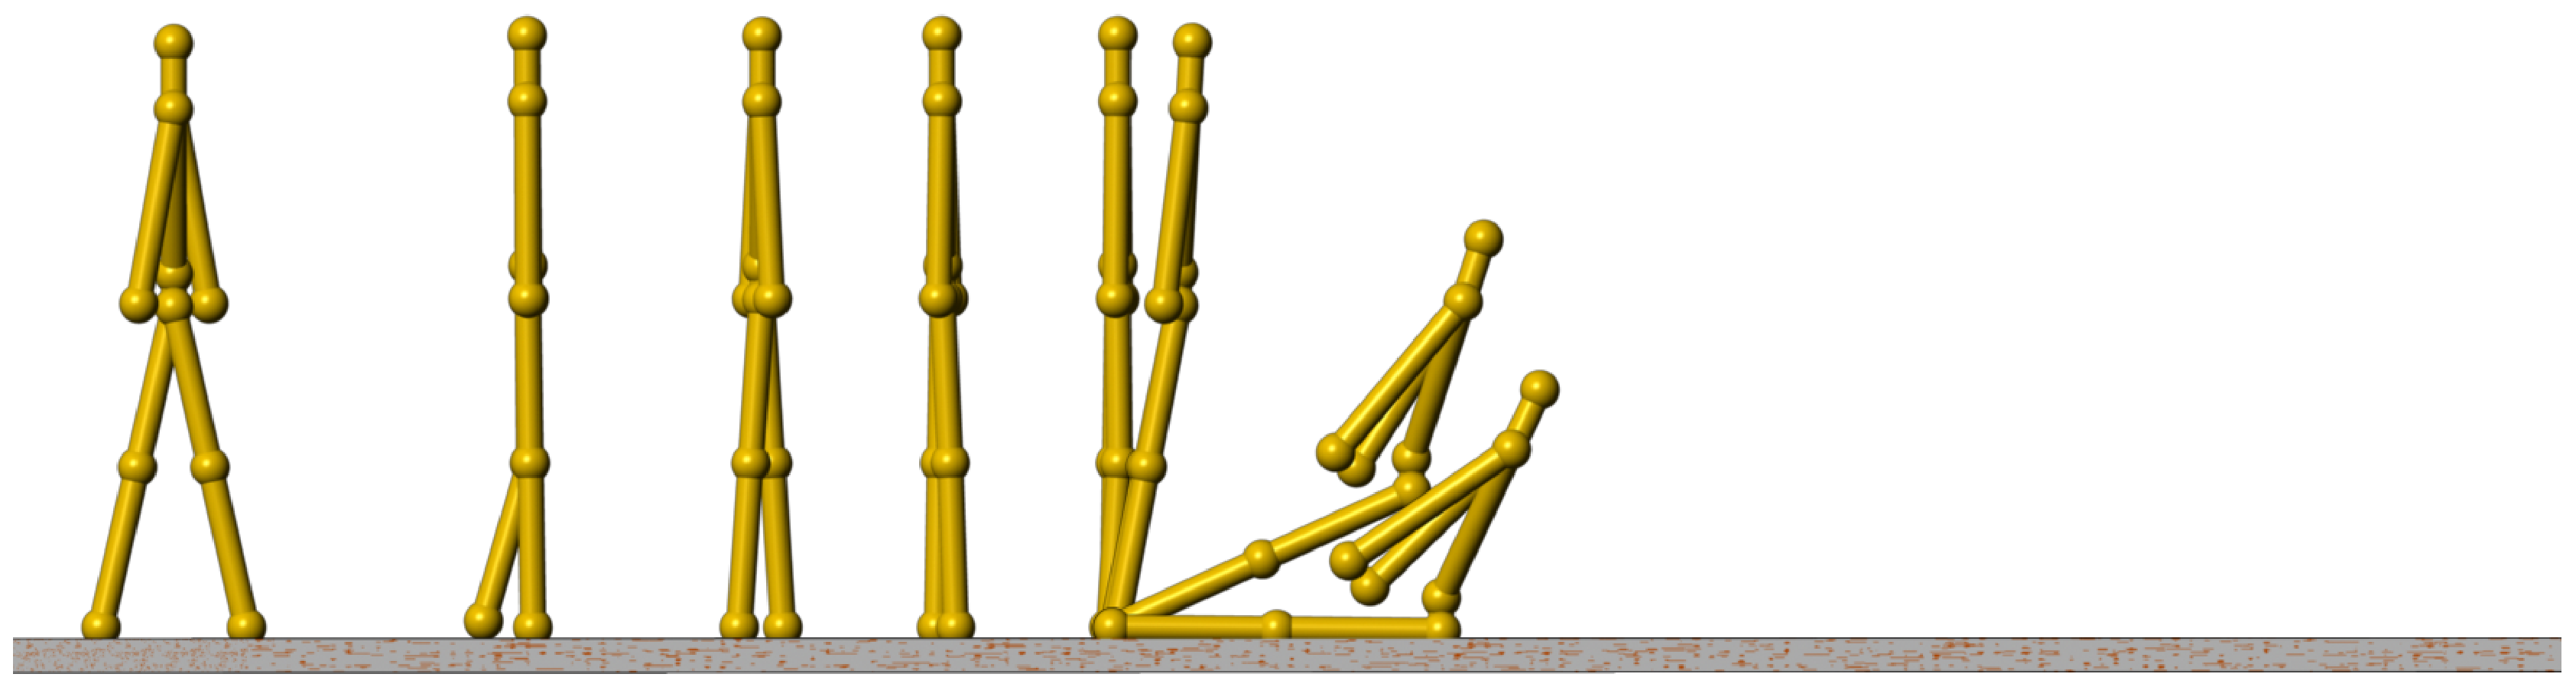
\includegraphics[height=6in]{walking_without_neural}
    \else
      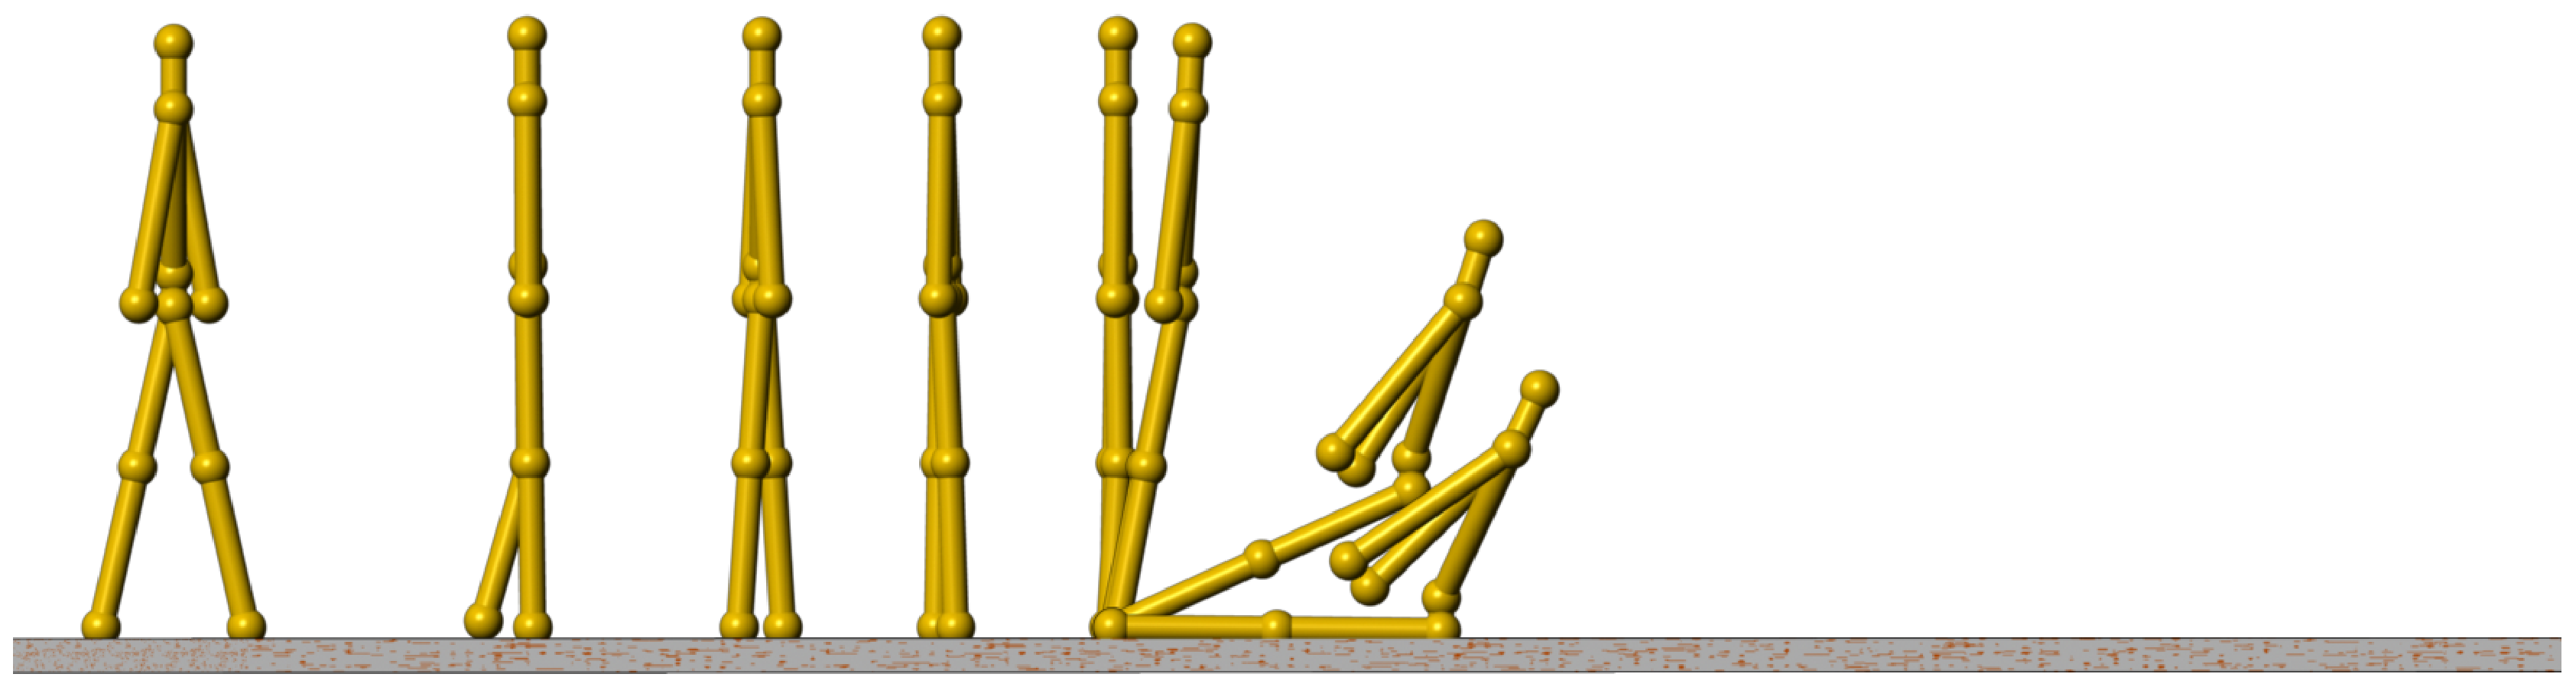
\includegraphics[width=0.7\textwidth]{walking_without_neural}
    \fi
    \caption{Without Neural Oscilator On Plain}
    \label{fig:fwalkingphase}
\end{center}
\end{figure}

\begin{figure}[!htbp]
  \begin{center}
    \leavevmode
    \ifpdf
      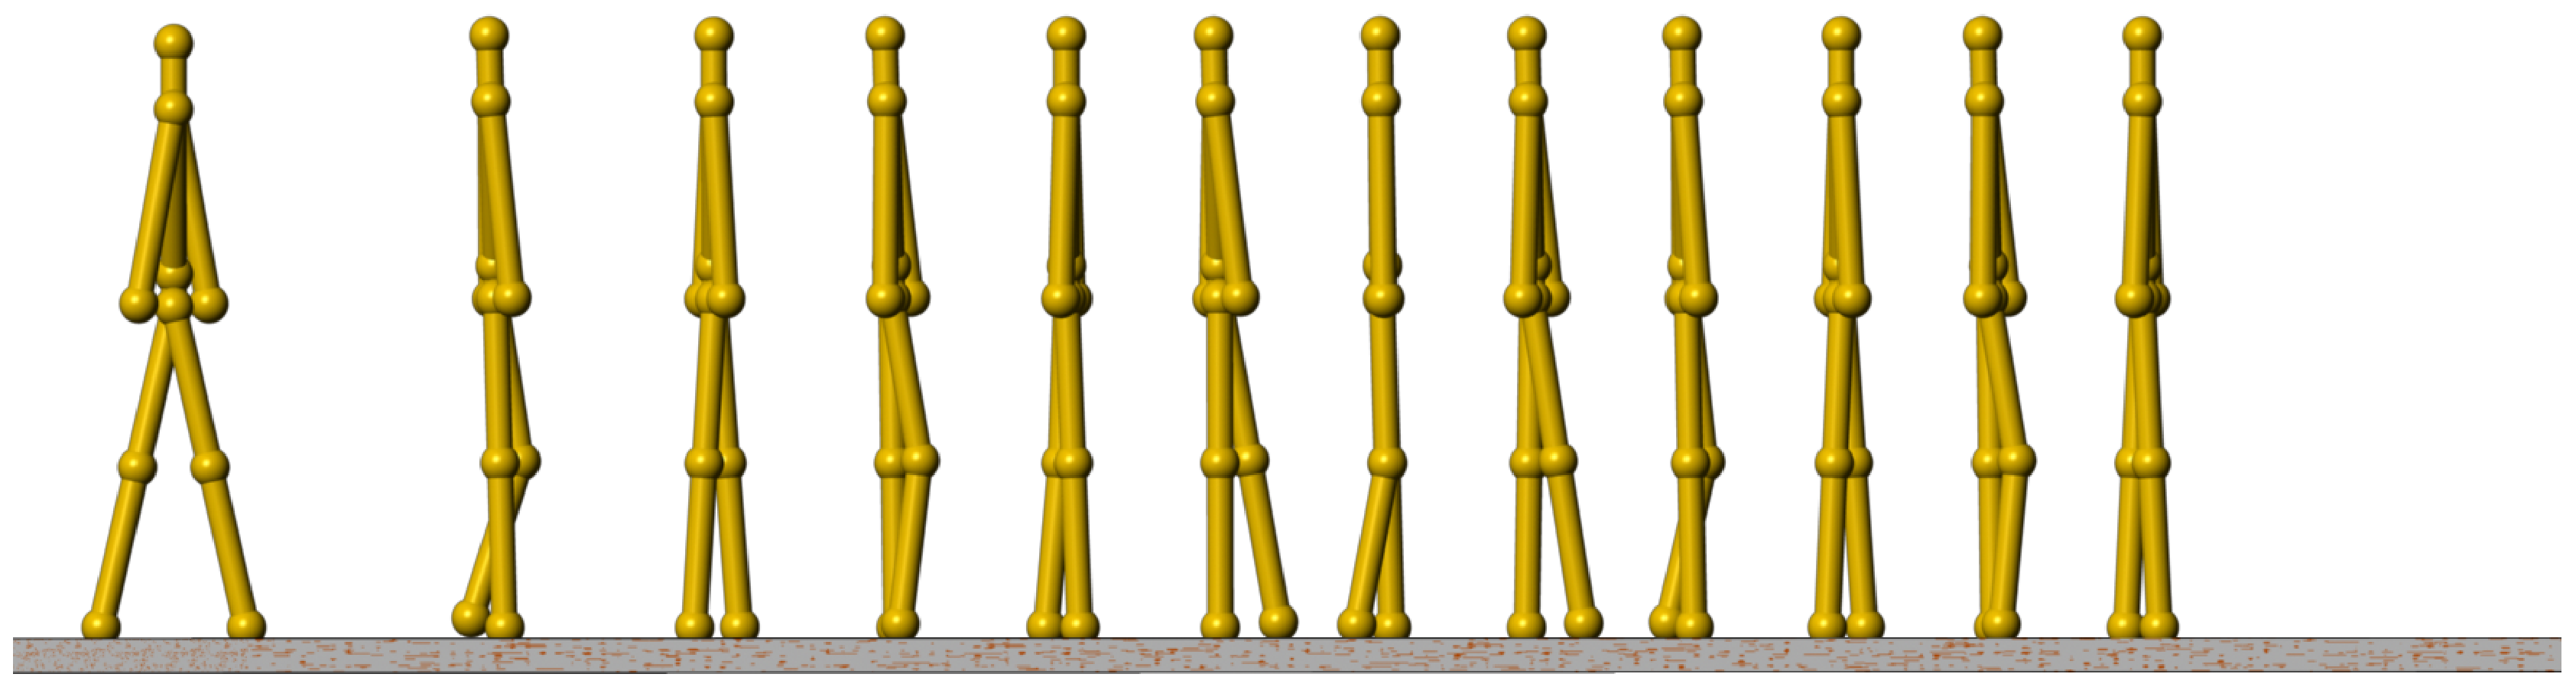
\includegraphics[height=6in]{walking_with_neural}
    \else
      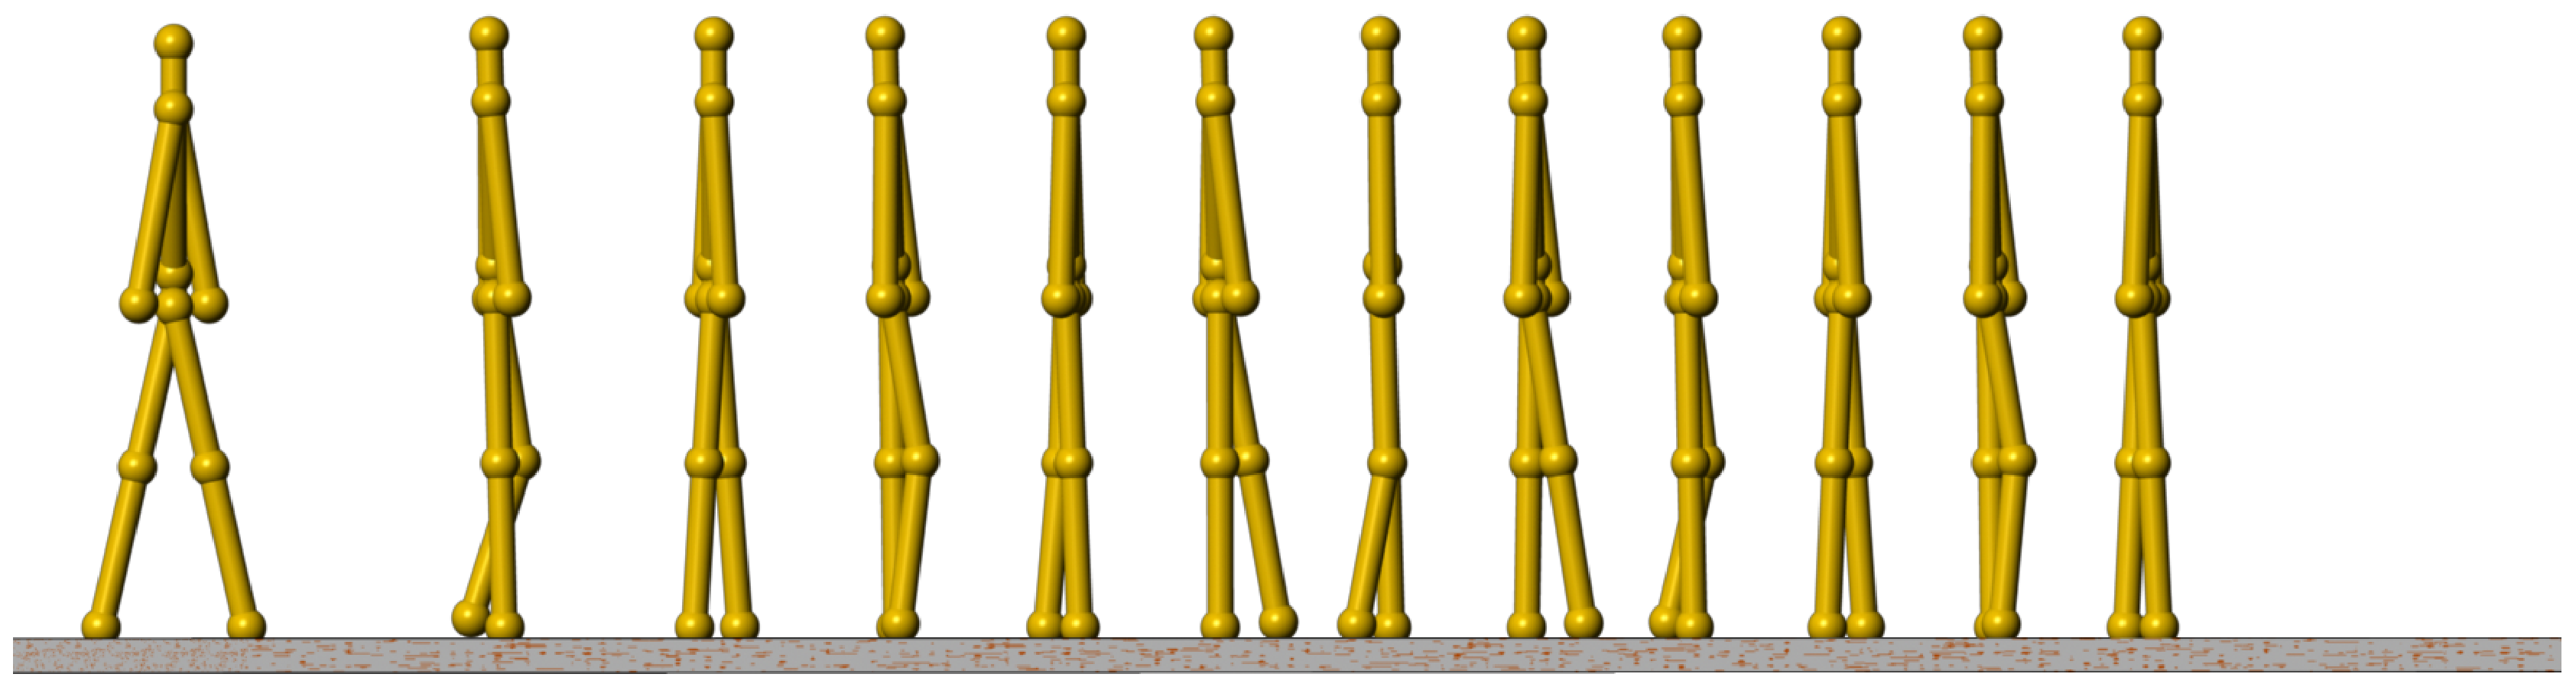
\includegraphics[width=0.7\textwidth]{walking_with_neural}
    \fi
    \caption{With Neural Oscilator on Plain}
    \label{fig:fourphaselimitcycle}
\end{center}
\end{figure}

\begin{figure}[!htbp]
  \begin{center}
    \leavevmode
    \ifpdf
      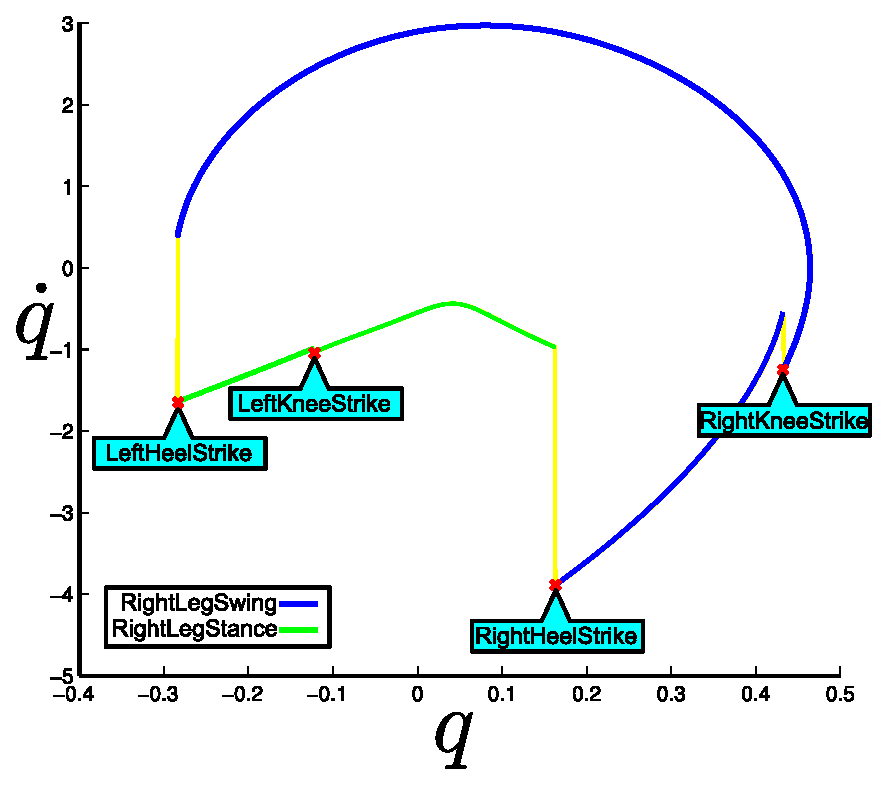
\includegraphics[height=6in]{walk_cycle_index}
    \else
      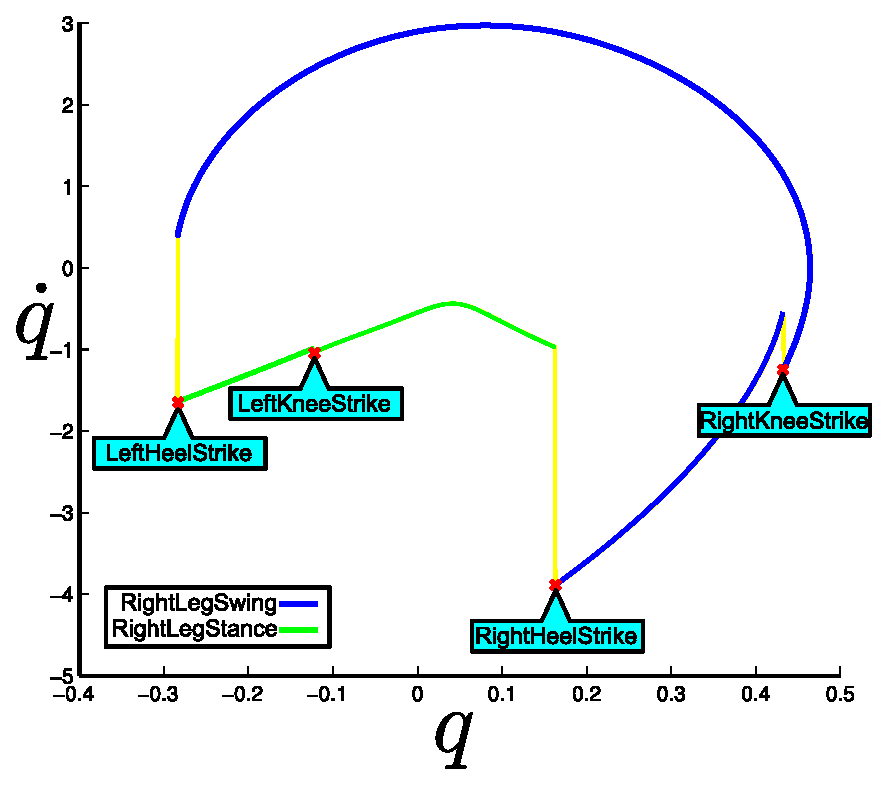
\includegraphics[width=0.7\textwidth]{walk_cycle_index}
    \fi
    \caption{Limit Circle And Different Phase in Passive Walking}
    \label{fig:fourphaselimitcycle}
\end{center}
\end{figure}


Also we can inclue the state perturbation by push the walker a little when it is walking.
it return to the stable walking cycle, this means the basin of attraction has been enlarged.





\subsection{System Gait Adaptation}
The passive dynamic system have many parameters, changing such parameters will generate different gait through sysmtem adaption.
we can fomulate the original system as
\[
\dot{\state}=F_a(\state)
\]
where $a$ is the system parameters.
we adjust the several parameters, neural oscillator maintain the limit cycle, but different parameters will generate different gait.
Some meaningfull gait are shown.
Becaus uniformally change the parameter will not effect the gaits, only will effect the period, so we most of the parameters we change is the ratio.
We wil maintain the leg length $L$ and mass sum.
\subsubsection*{Mass Distribution Change}
We change the mass of the hip $m_h$, different $m_h$ will generate different gaits, while bigger $m_h$ wil result motion that are similar to burdenned gait.
different Limit Cycles are show in Figure ~\ref{fig_differentmh}
\begin{figure}[!htbp]
  \begin{center}
    \leavevmode
    \ifpdf
      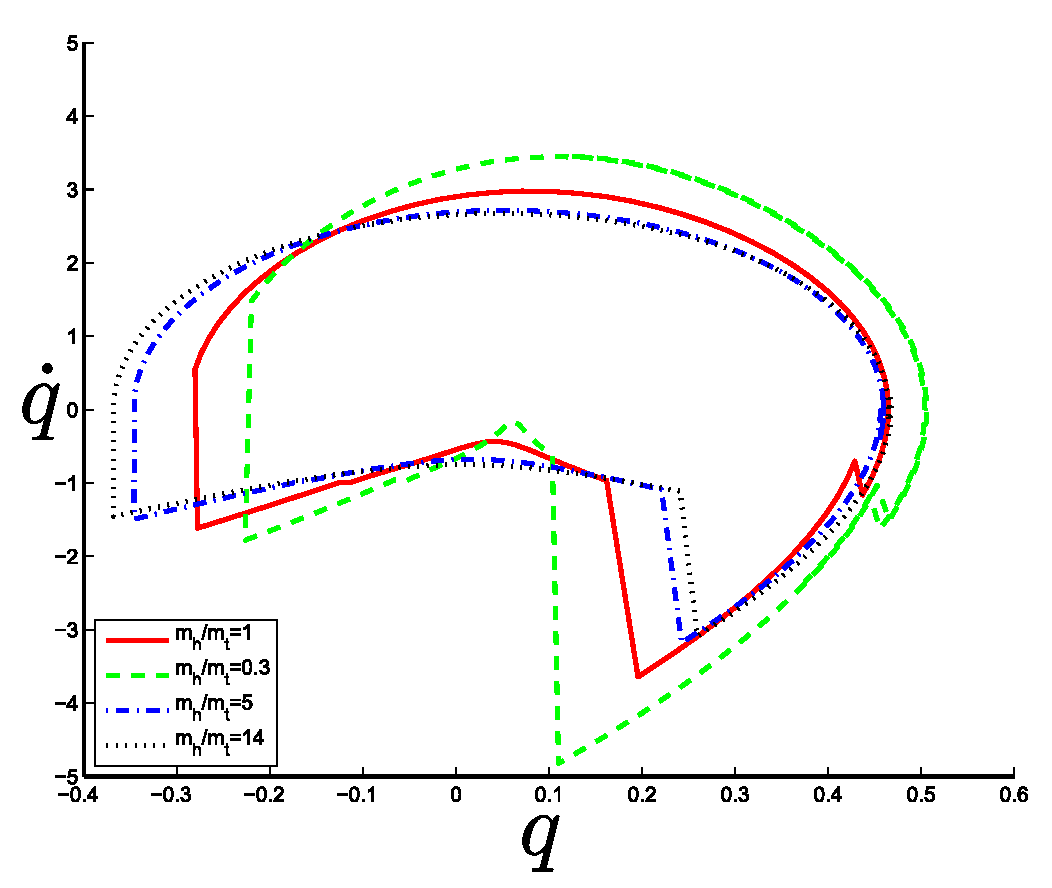
\includegraphics[height=6in]{MassDistributionEffectsOnLimitCircle}
    \else
      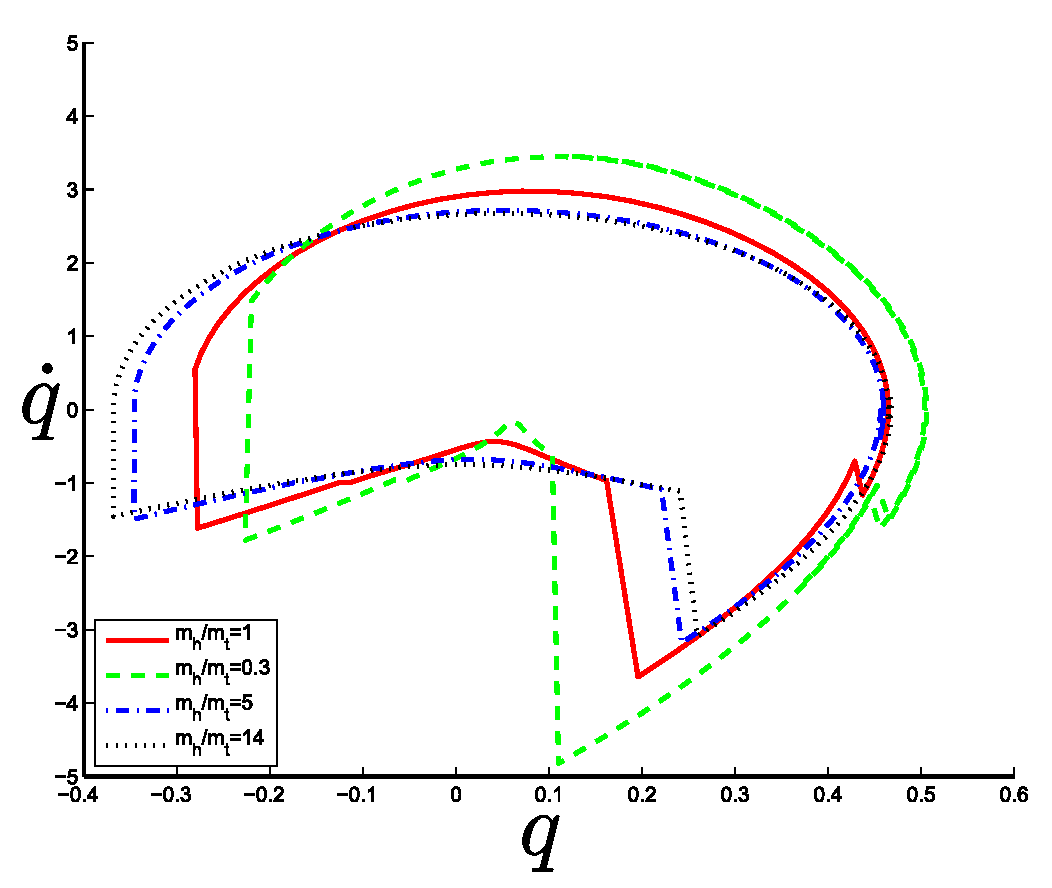
\includegraphics[width=0.7\textwidth]{MassDistributionEffectsOnLimitCircle}
    \fi
    \caption{Different Gait Resulting From the Different Mass Ratio}
    \label{fig:differentmh}
\end{center}
\end{figure}

From the phase plot, we find some interesting tendency,
when the hip is heavier, it will walk with bigger step but a slow speed($\qd$ is lower),and also character tend to fall backward.
which the body is become litter, charater will waker with quickly($\qd$ is bigger) and it tends to lean forward.

This may give us some infomation about the upper body motion.
Usually, when we carry something heavier, we  tend to bend the body upper forward to prevent following backward.

different gaits are show in the following pictures.
\begin{figure}[!htbp]
  \begin{center}
      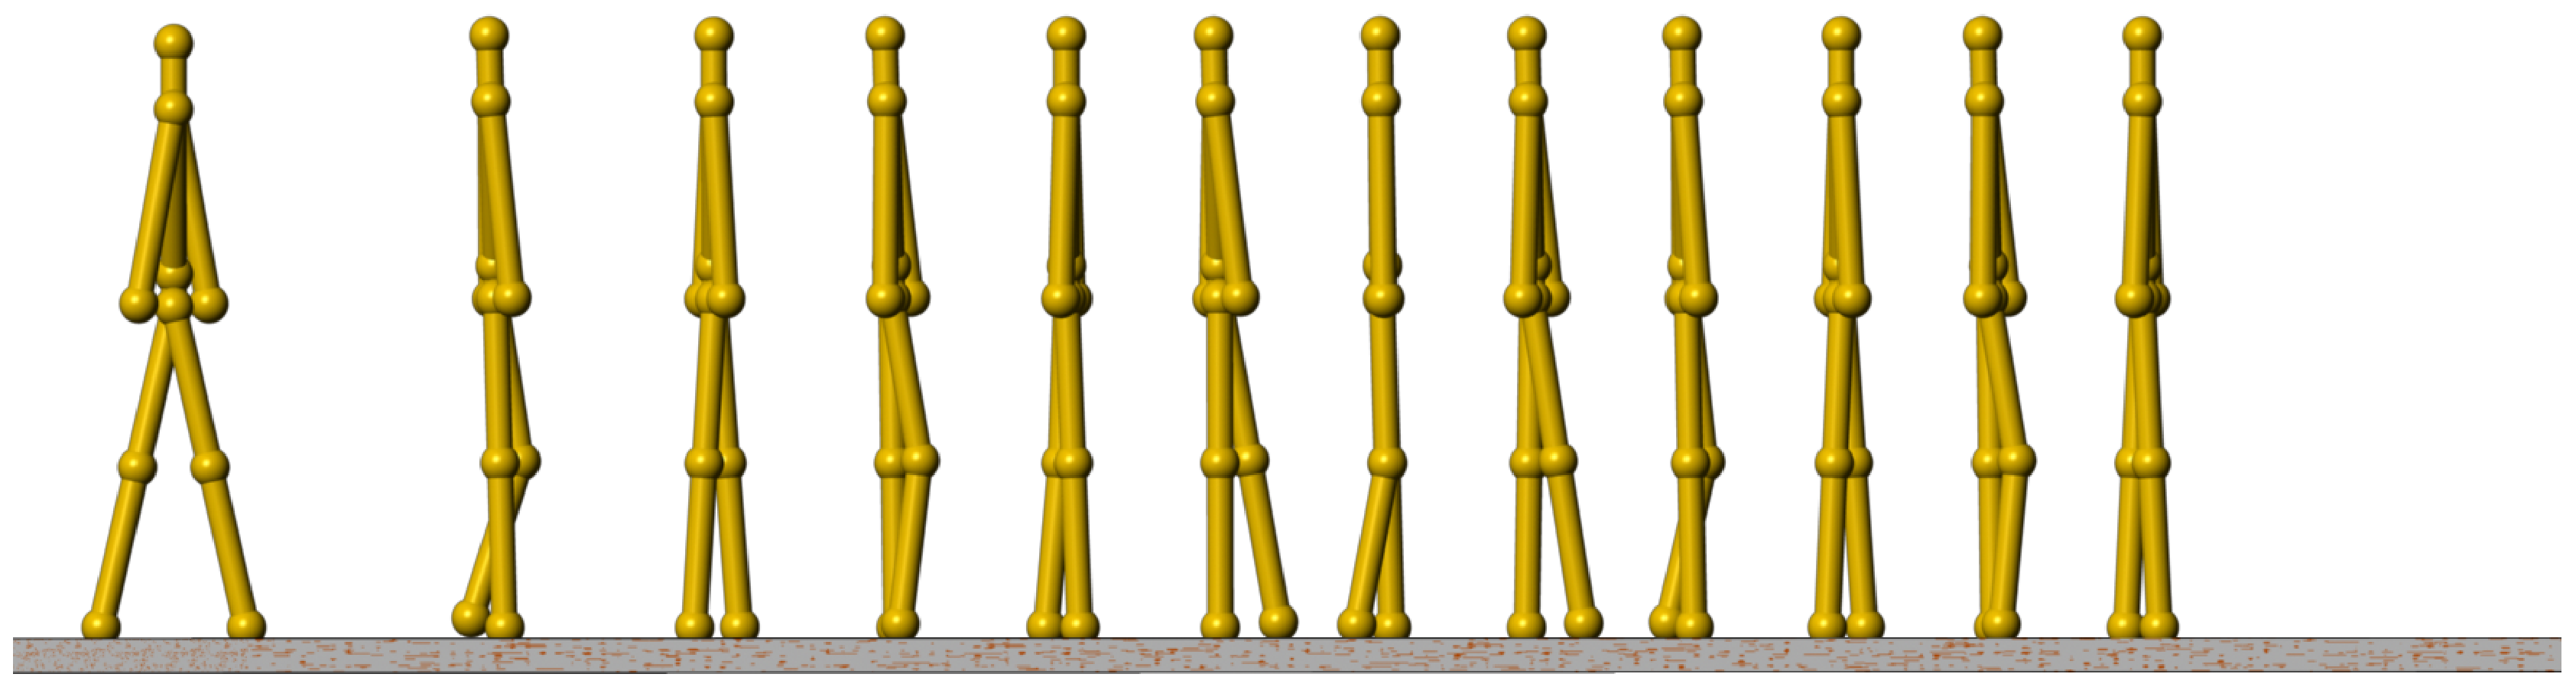
\includegraphics[width=0.7\textwidth]{walking_with_neural}
    \caption{Place Holder}
    \label{fig:massh1}
\end{center}
\end{figure}

\begin{figure}[!htbp]
  \begin{center}
      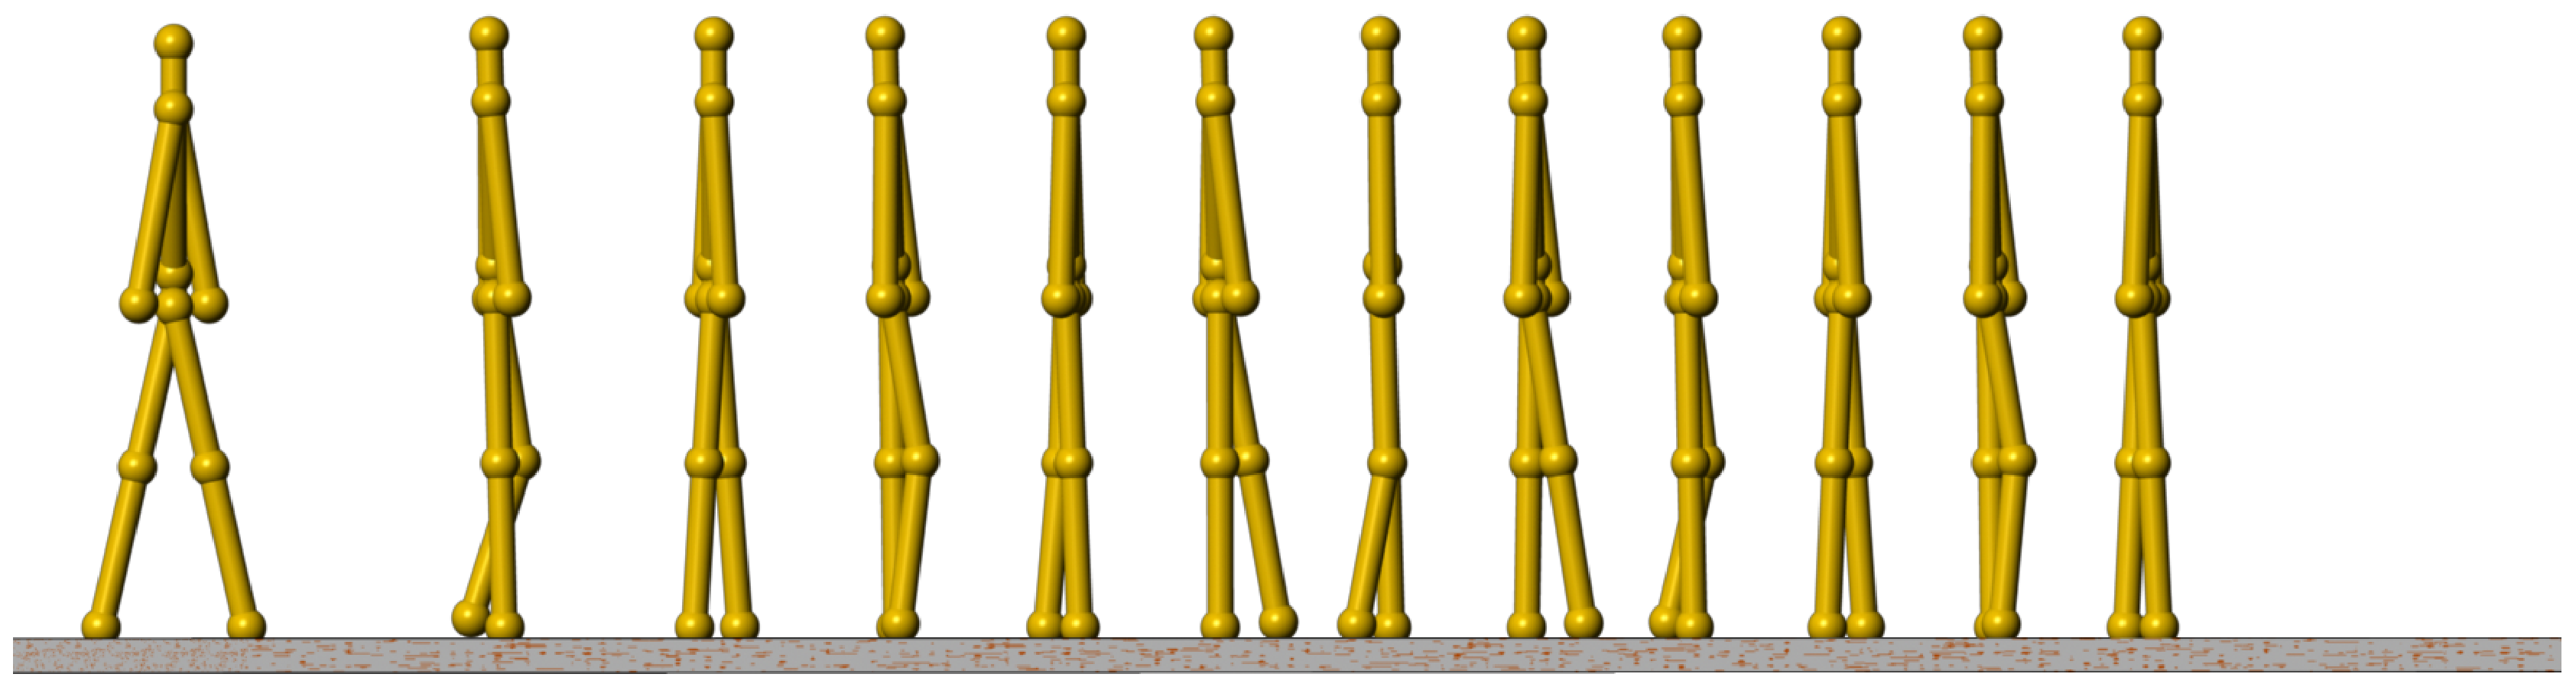
\includegraphics[width=0.7\textwidth]{walking_with_neural}
    \caption{Place Holder}
    \label{fig:massh2}
\end{center}
\end{figure}

\begin{figure}[!htbp]
  \begin{center}
      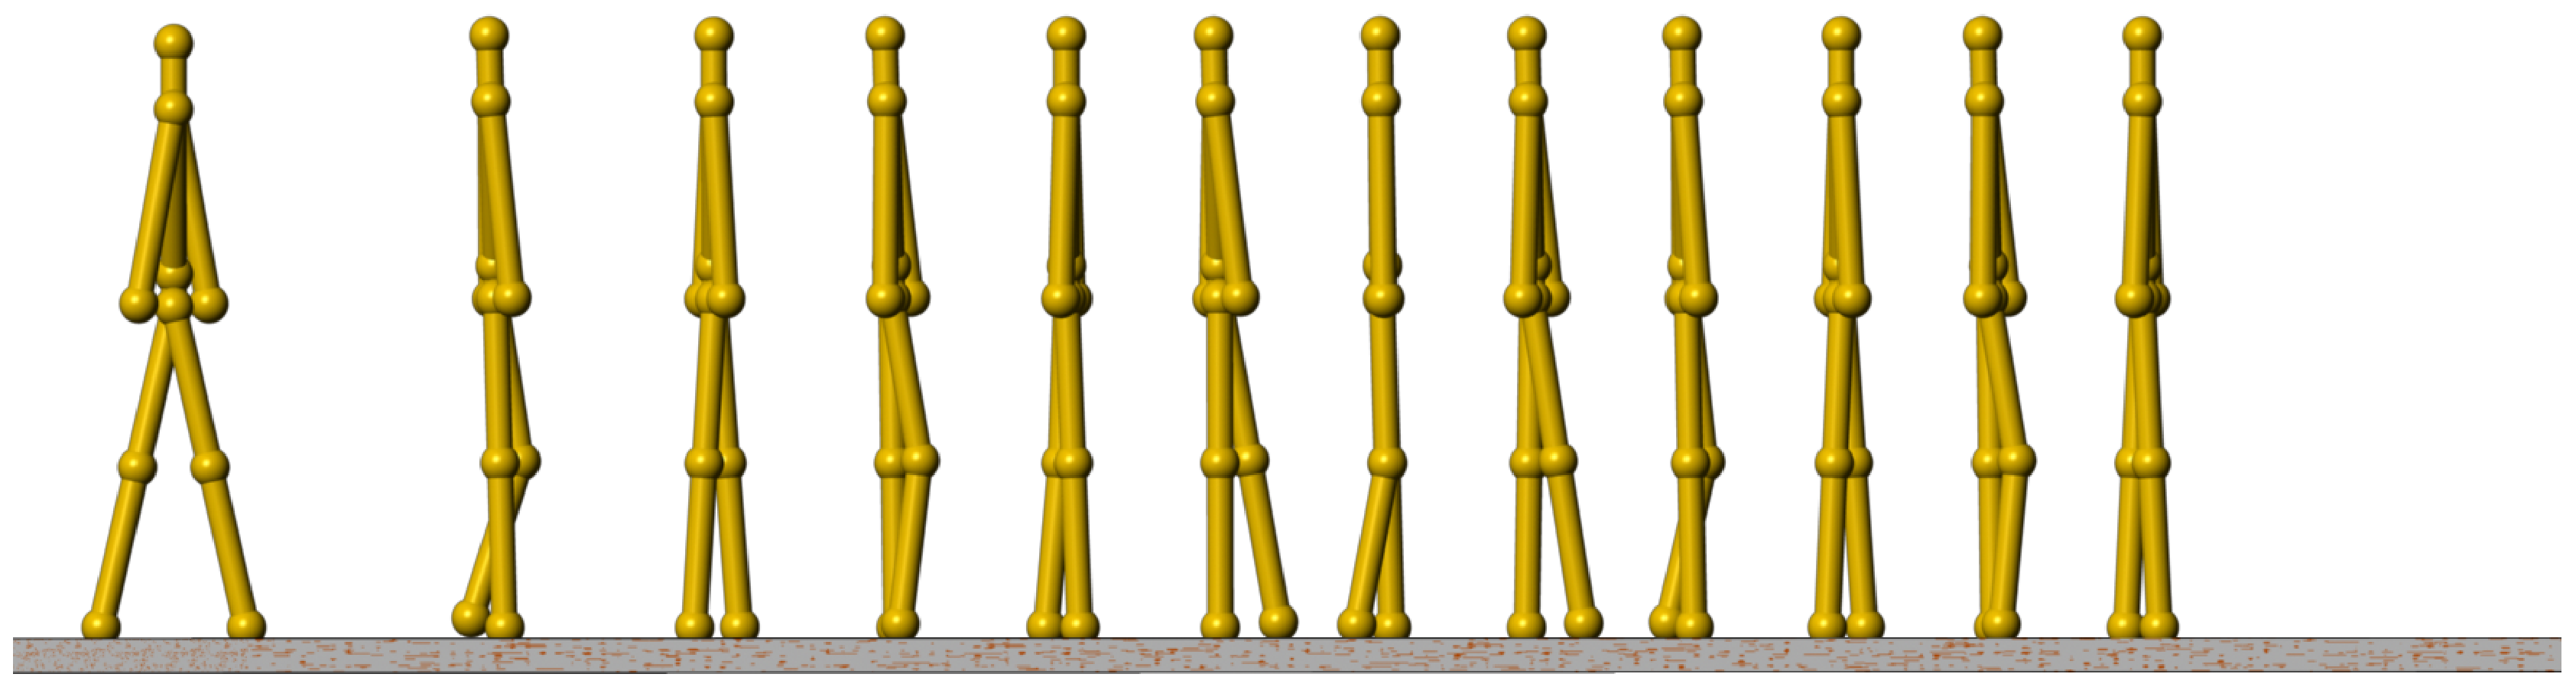
\includegraphics[width=0.7\textwidth]{walking_with_neural}
    \caption{Place Holder}
    \label{fig:massh3}
\end{center}
\end{figure}

%Mh/Mt=0.3

%Mh/Mt=2

%Mh/Mt=3

	
%Mh/mt=10


\subsubsection*{Leg Length Distribution Change}
we keep the leg length unchanged, but alter the ration of shank and thigh.
We generate gait with different leg length ratio.
as shown in figure~\ref{fig:differentlr}

\begin{figure}[!htbp]
  \begin{center}
    \leavevmode
    \ifpdf
      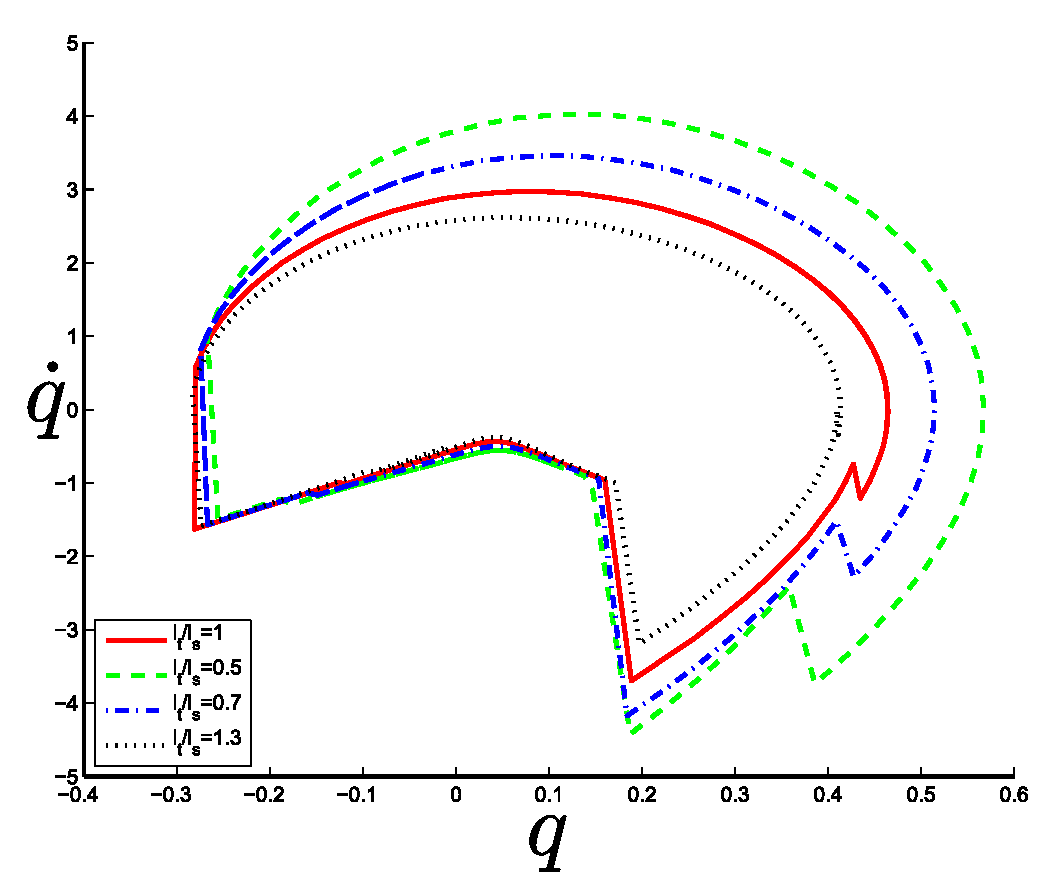
\includegraphics[height=6in]{LegLengthDistributionEffectsOnLimitCircle}
    \else
      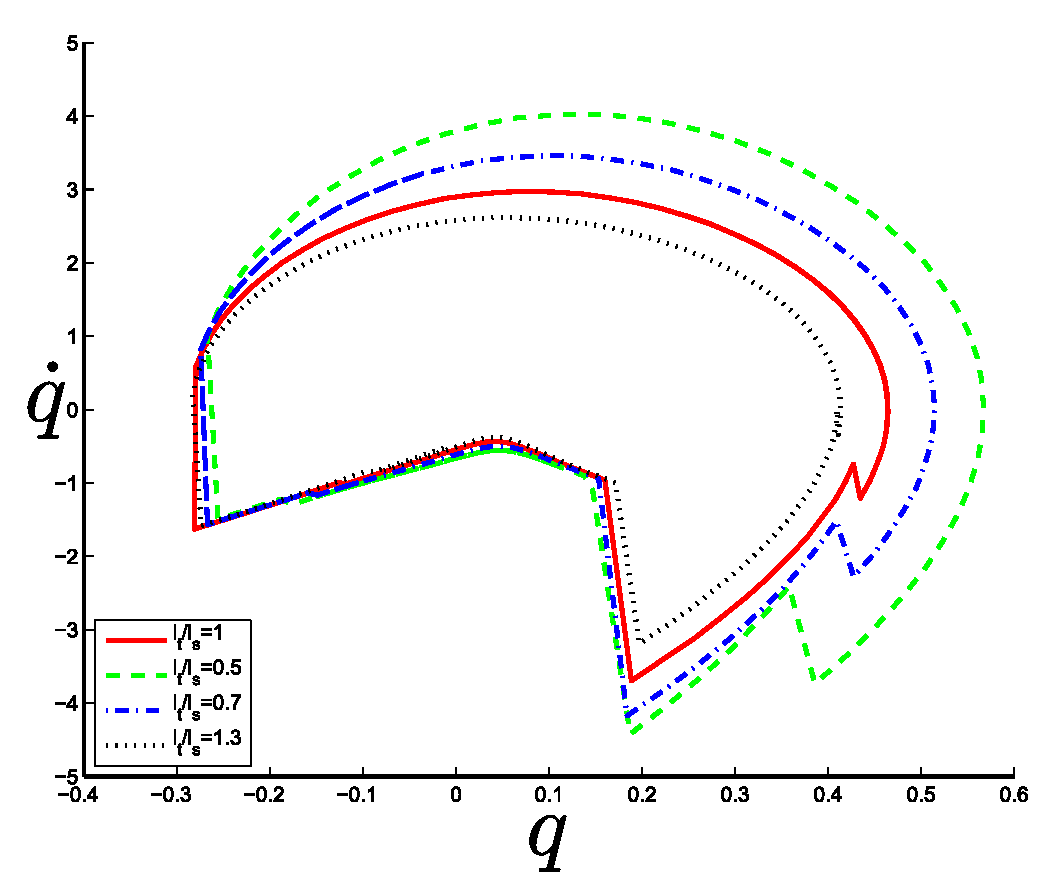
\includegraphics[width=0.7\textwidth]{LegLengthDistributionEffectsOnLimitCircle}
    \fi
    \caption{Different Gait Resulting From the Different Mass Ratio}
    \label{fig:differentlr}
\end{center}
\end{figure}

for the limit cycle in figure~\ref{fig:differentlr}, we find something interesing.
Basically, the support leg motion is almost the same, while different leg length ration will result in different sway angle
basically the longger the shank, thigh has to sway quickly and with bigger amplitude.
There are aslo bigger impulse during the strike phase. For both the knee and heel strike, larger impulse is generated.
while step size is kept.
This maybe true that girls walking with tall heel will easilly get knees and heel injured and aslo will generate larger step sound.


\begin{figure}[!htbp]
  \begin{center}
      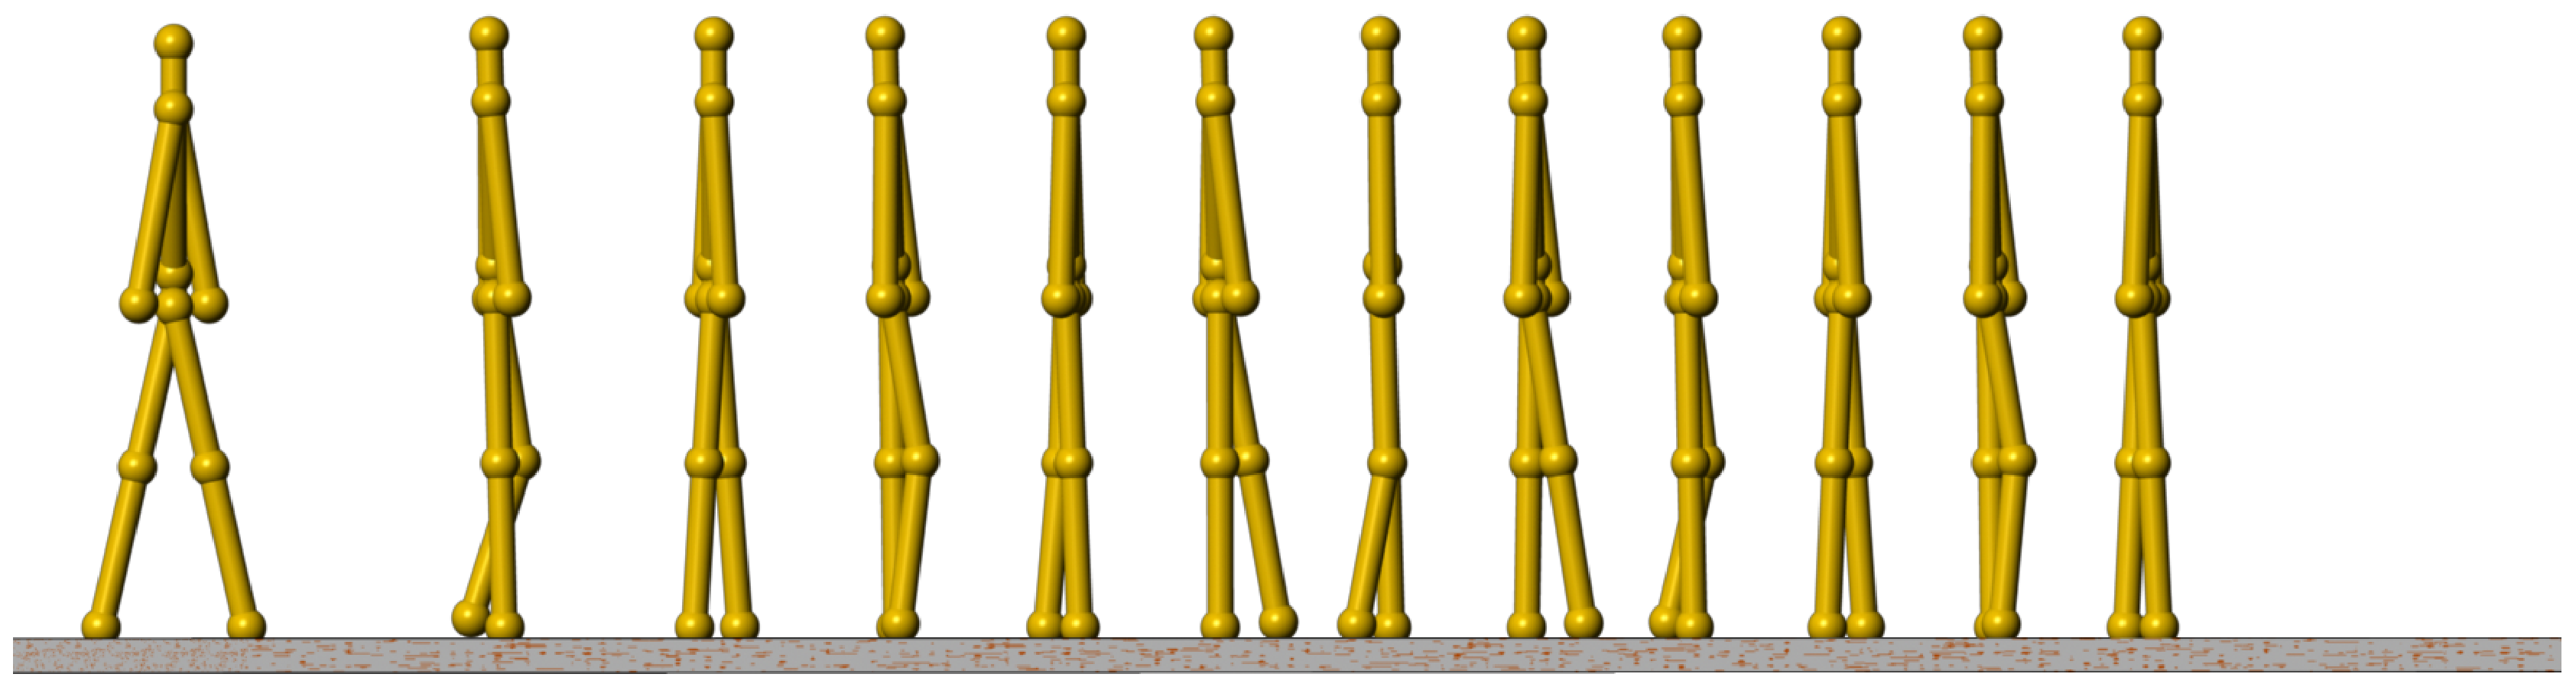
\includegraphics[width=0.7\textwidth]{walking_with_neural}
    \caption{Place Holder1}
    \label{fig:lr1}
\end{center}
\end{figure}

\begin{figure}[!htbp]
  \begin{center}
      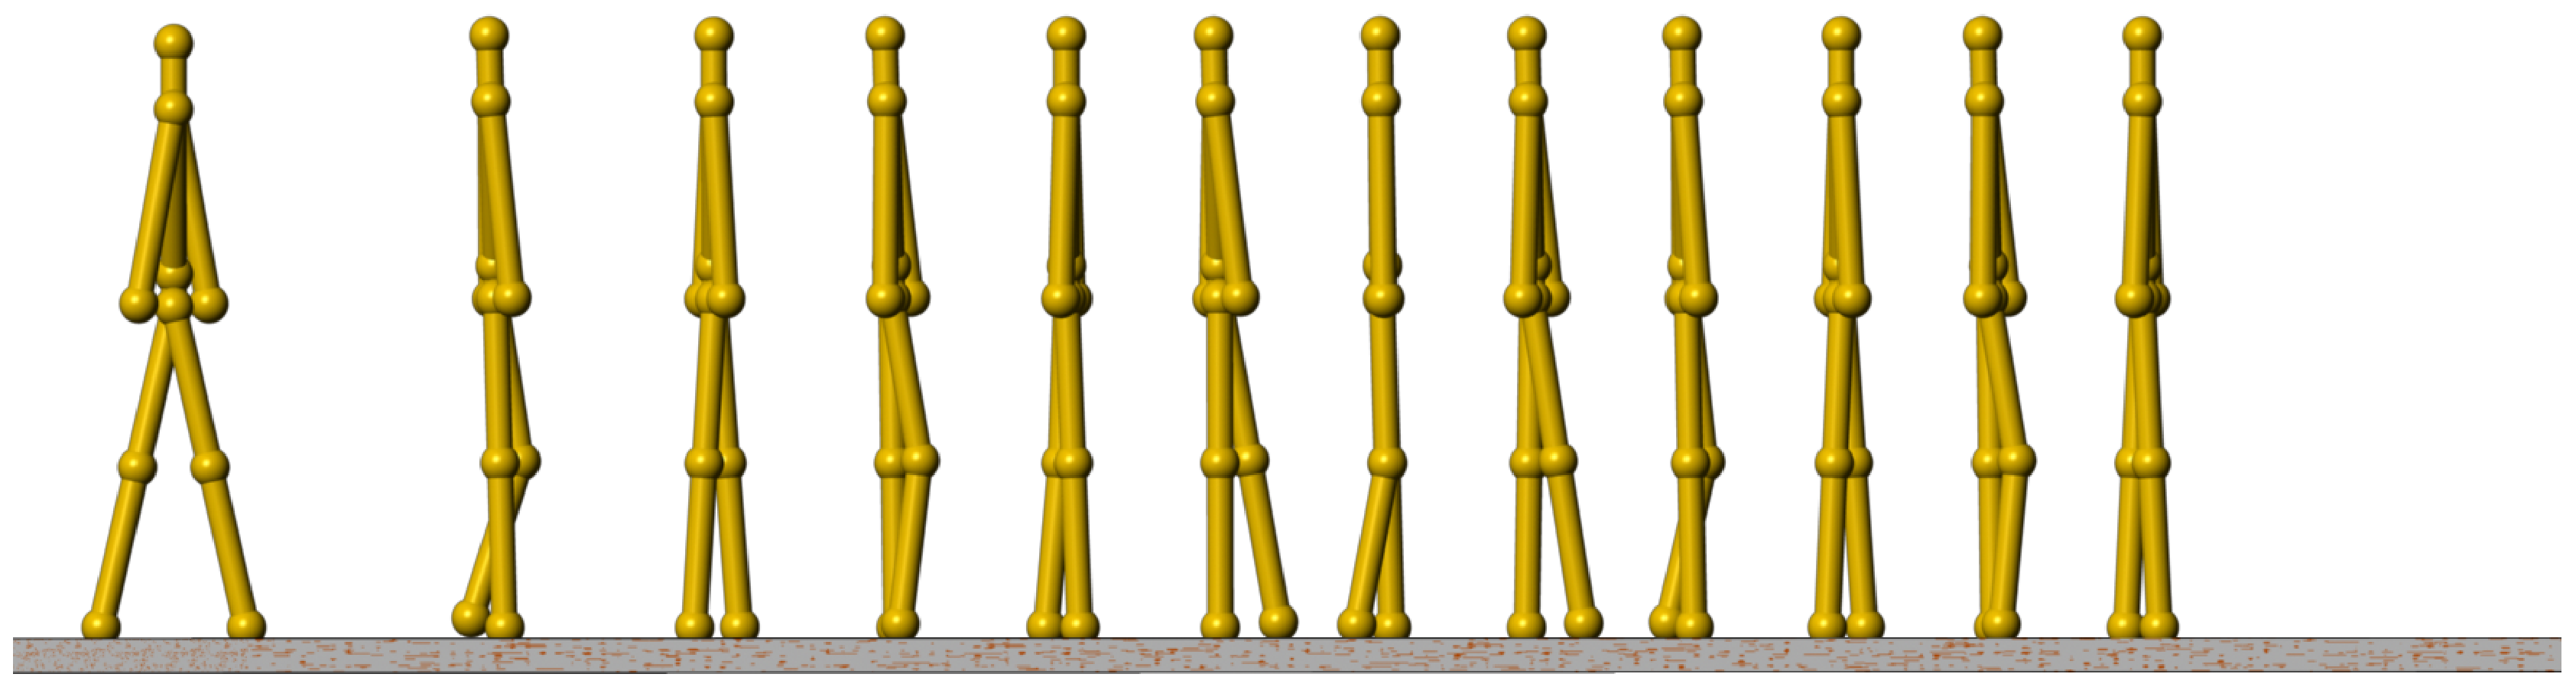
\includegraphics[width=0.7\textwidth]{walking_with_neural}
    \caption{Place Holder2}
    \label{fig:lr2}
\end{center}
\end{figure}

\begin{figure}[!htbp]
  \begin{center}
      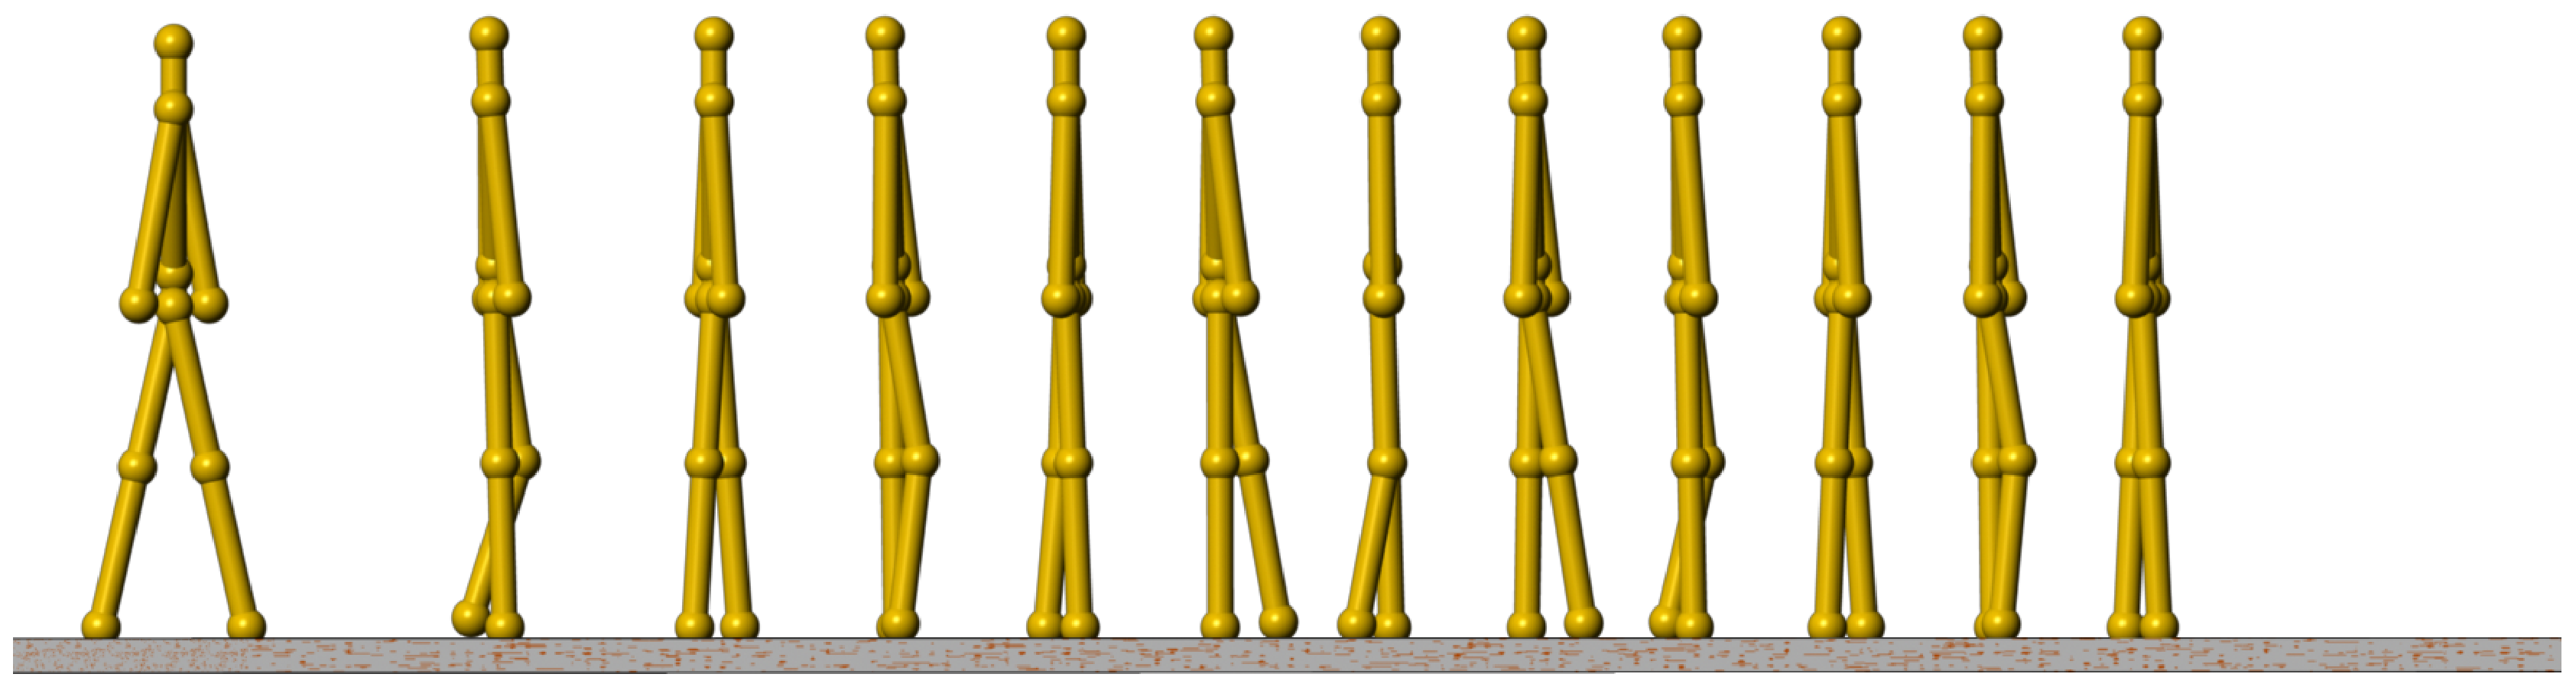
\includegraphics[width=0.7\textwidth]{walking_with_neural}
    \caption{Place Holder3}
    \label{fig:lr3}
\end{center}
\end{figure}




\subsubsection*{SlopChange}
Also we can change different downslope.
For different slope, entrainment maintained the limit cycle, but limit cycle changed its shape.
different stable limit circles are show in figure ~\ref{fig:diffstepsize}
basically ,the bigger the slope, the bigger the step size the higher the speed, and produce a gait similar to energy scaling.

\begin{figure}[!htbp]
  \begin{center}
    \leavevmode
    \ifpdf
      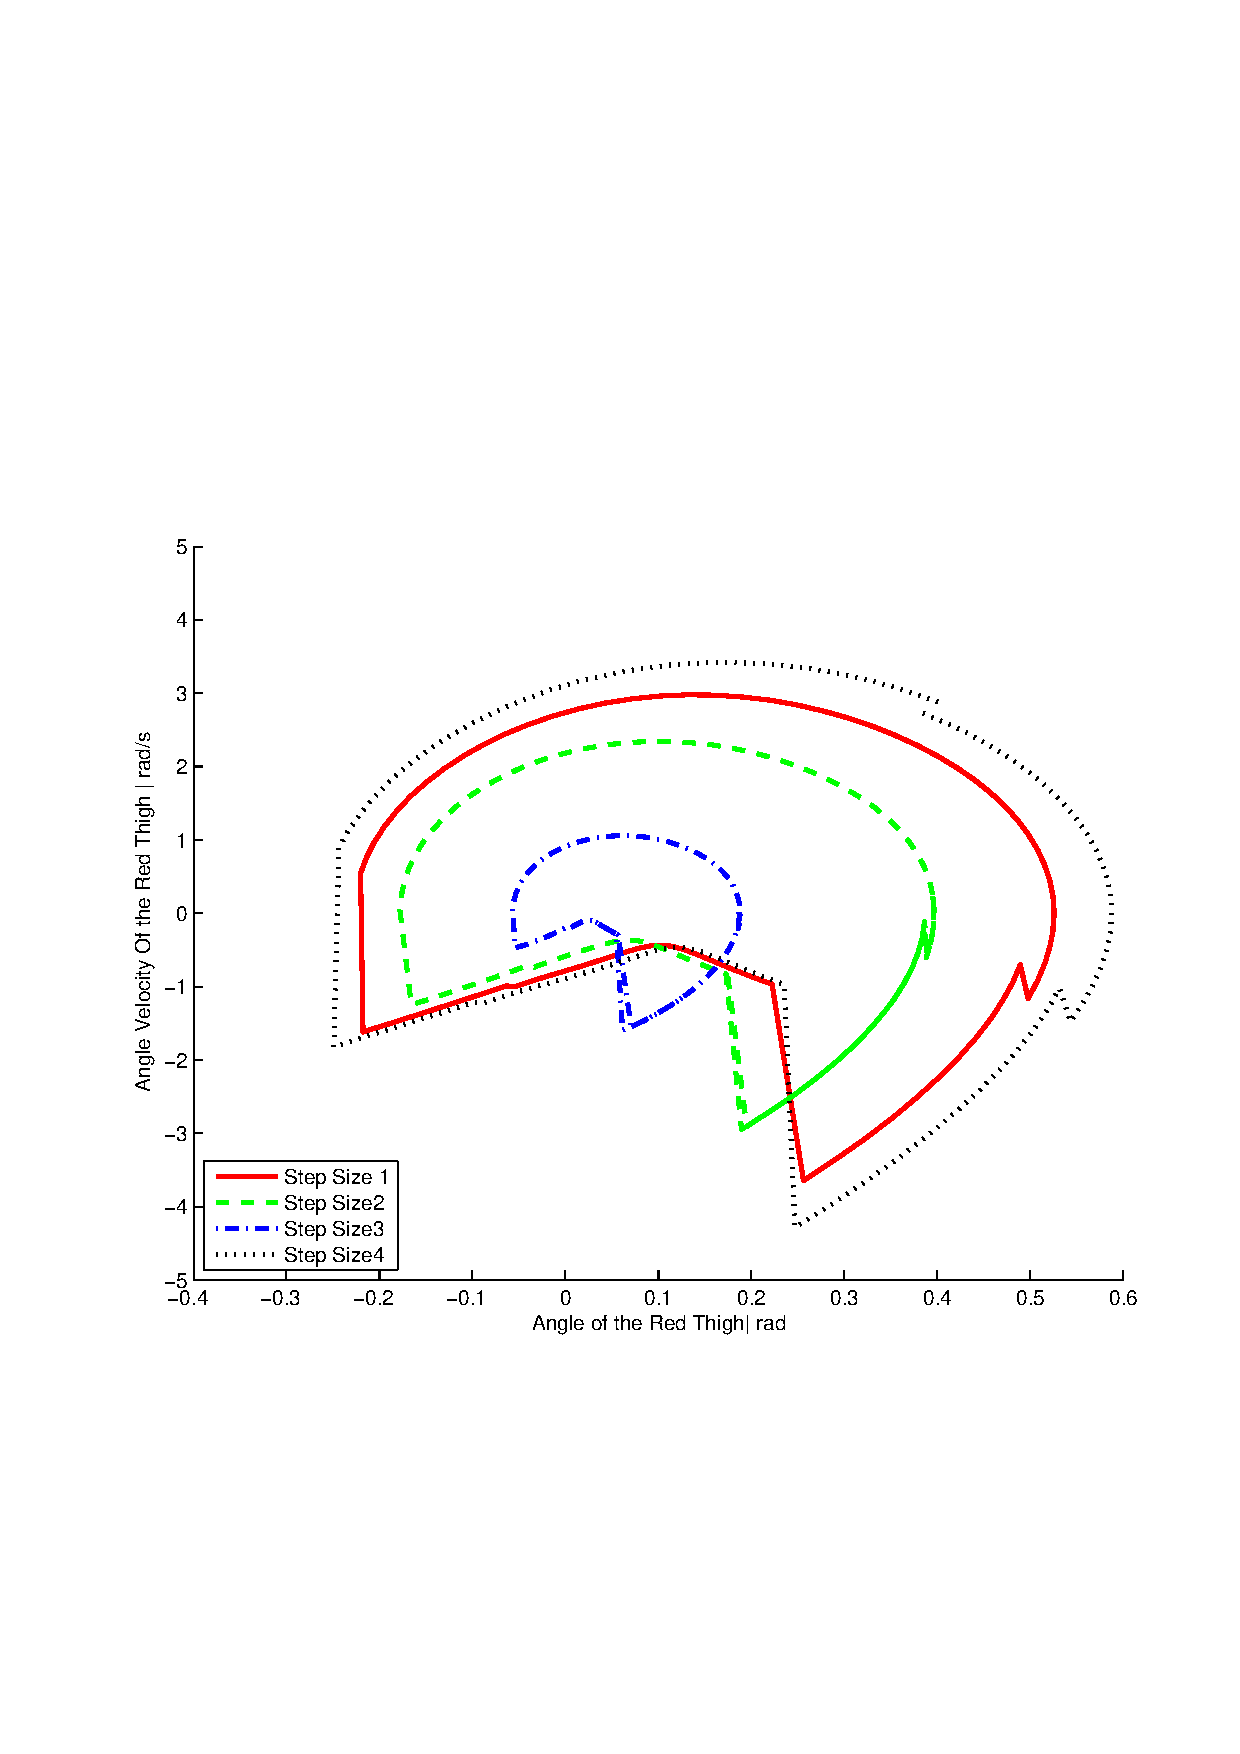
\includegraphics[height=6in]{DifferentStepSizeWalking}
    \else
      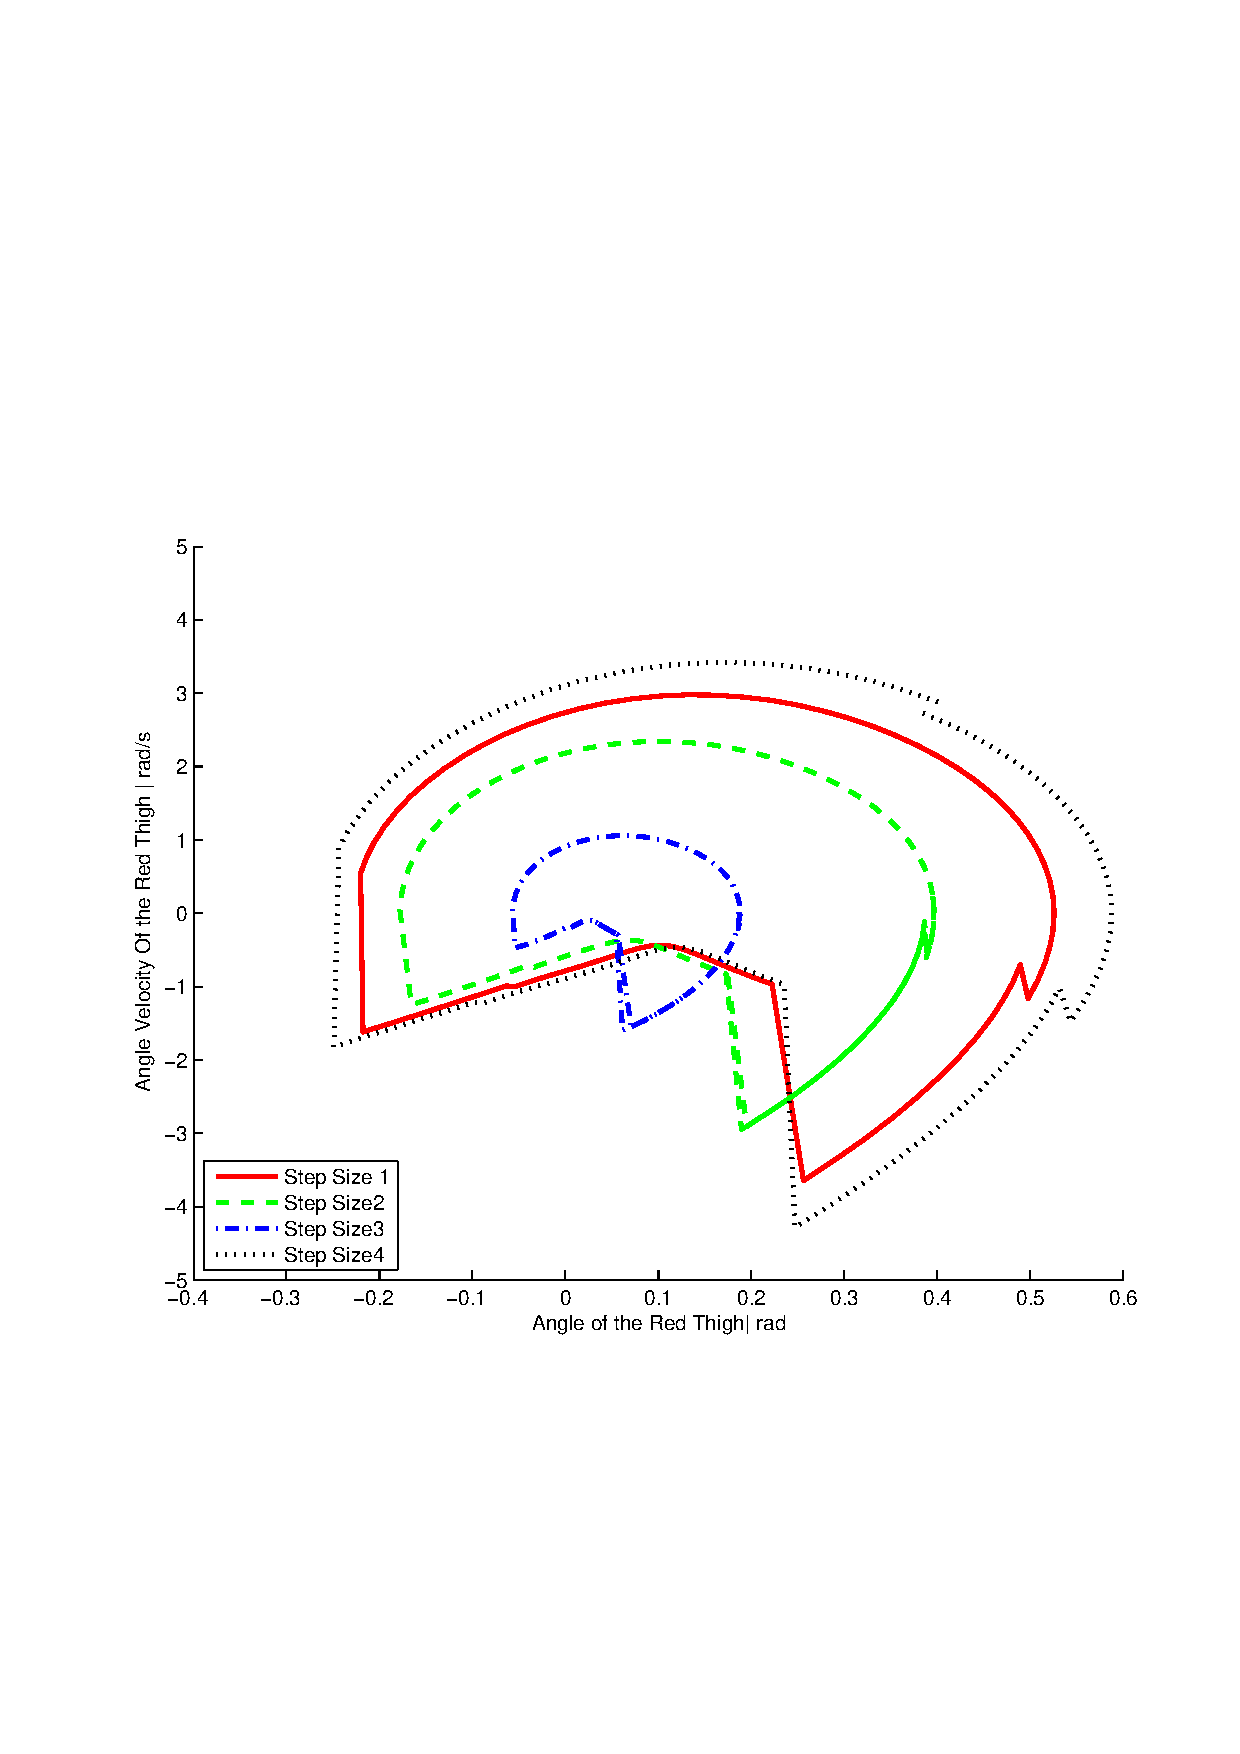
\includegraphics[width=0.7\textwidth]{DifferentStepSizeWalking}
    \fi
    \caption{different step size walking}
    \label{fig:differentlr}
\end{center}
\end{figure}


\begin{figure}[!htbp]
  \begin{center}
      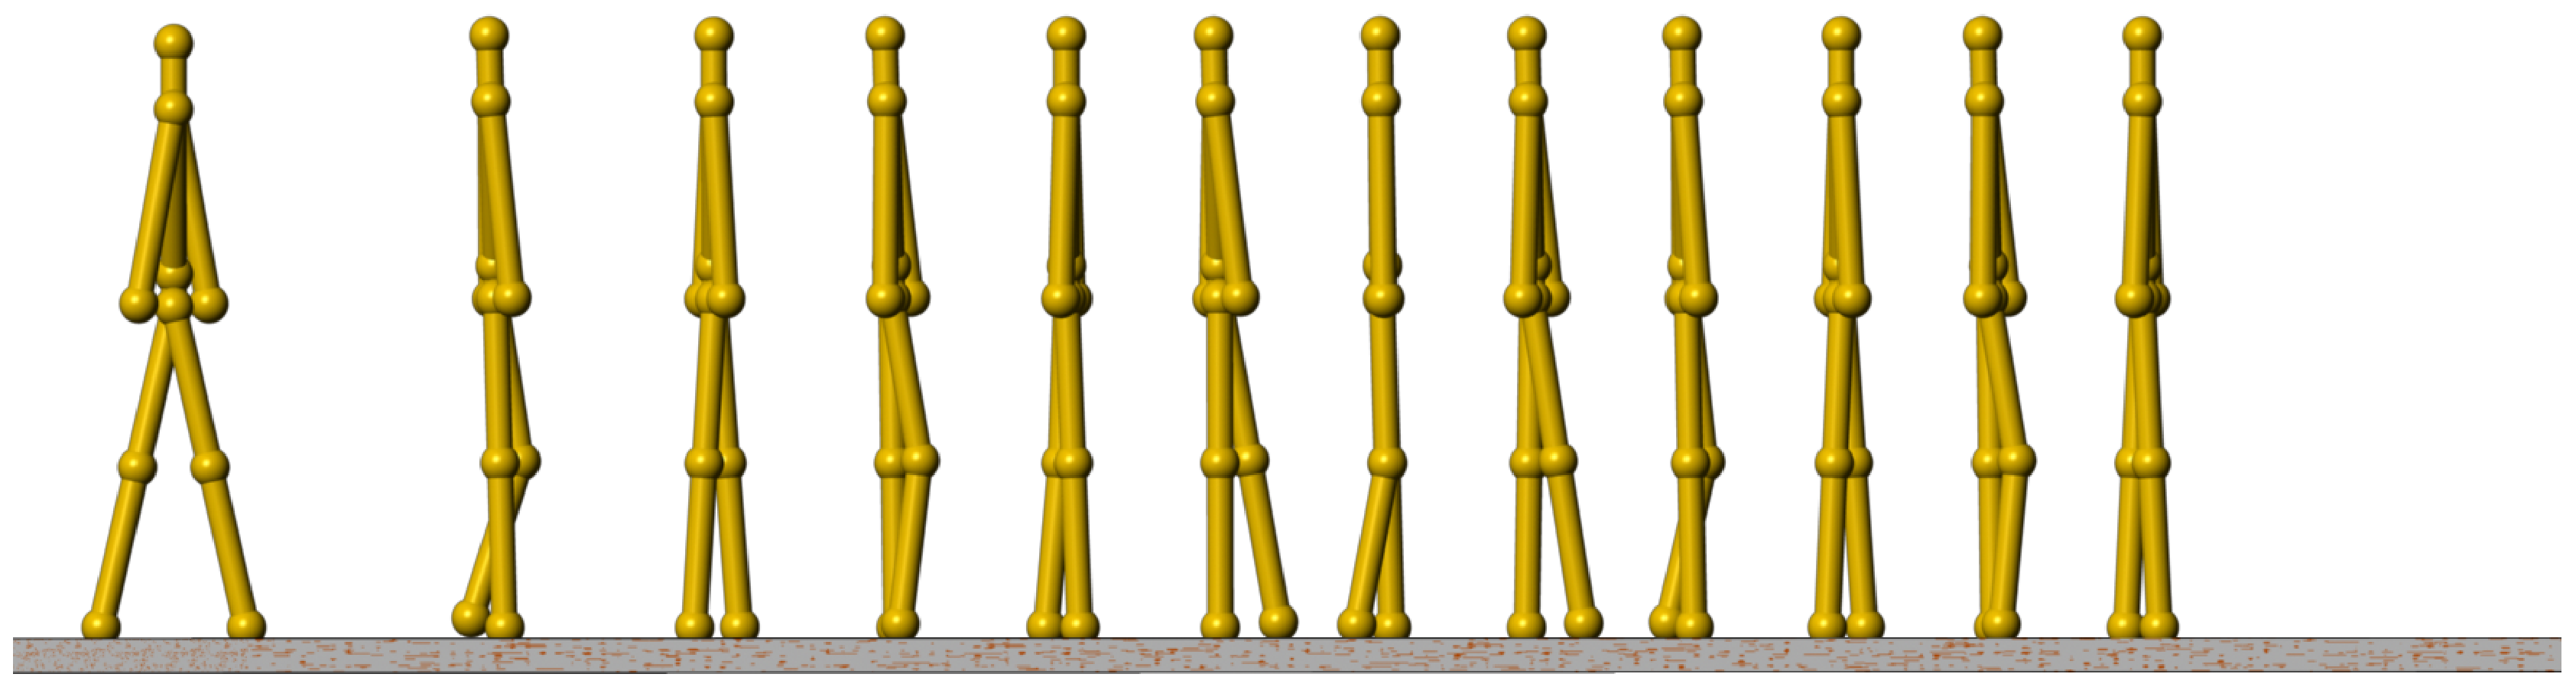
\includegraphics[width=0.7\textwidth]{walking_with_neural}
    \caption{Place Holder1}
    \label{fig:ss1}
\end{center}
\end{figure}

\begin{figure}[!htbp]
  \begin{center}
      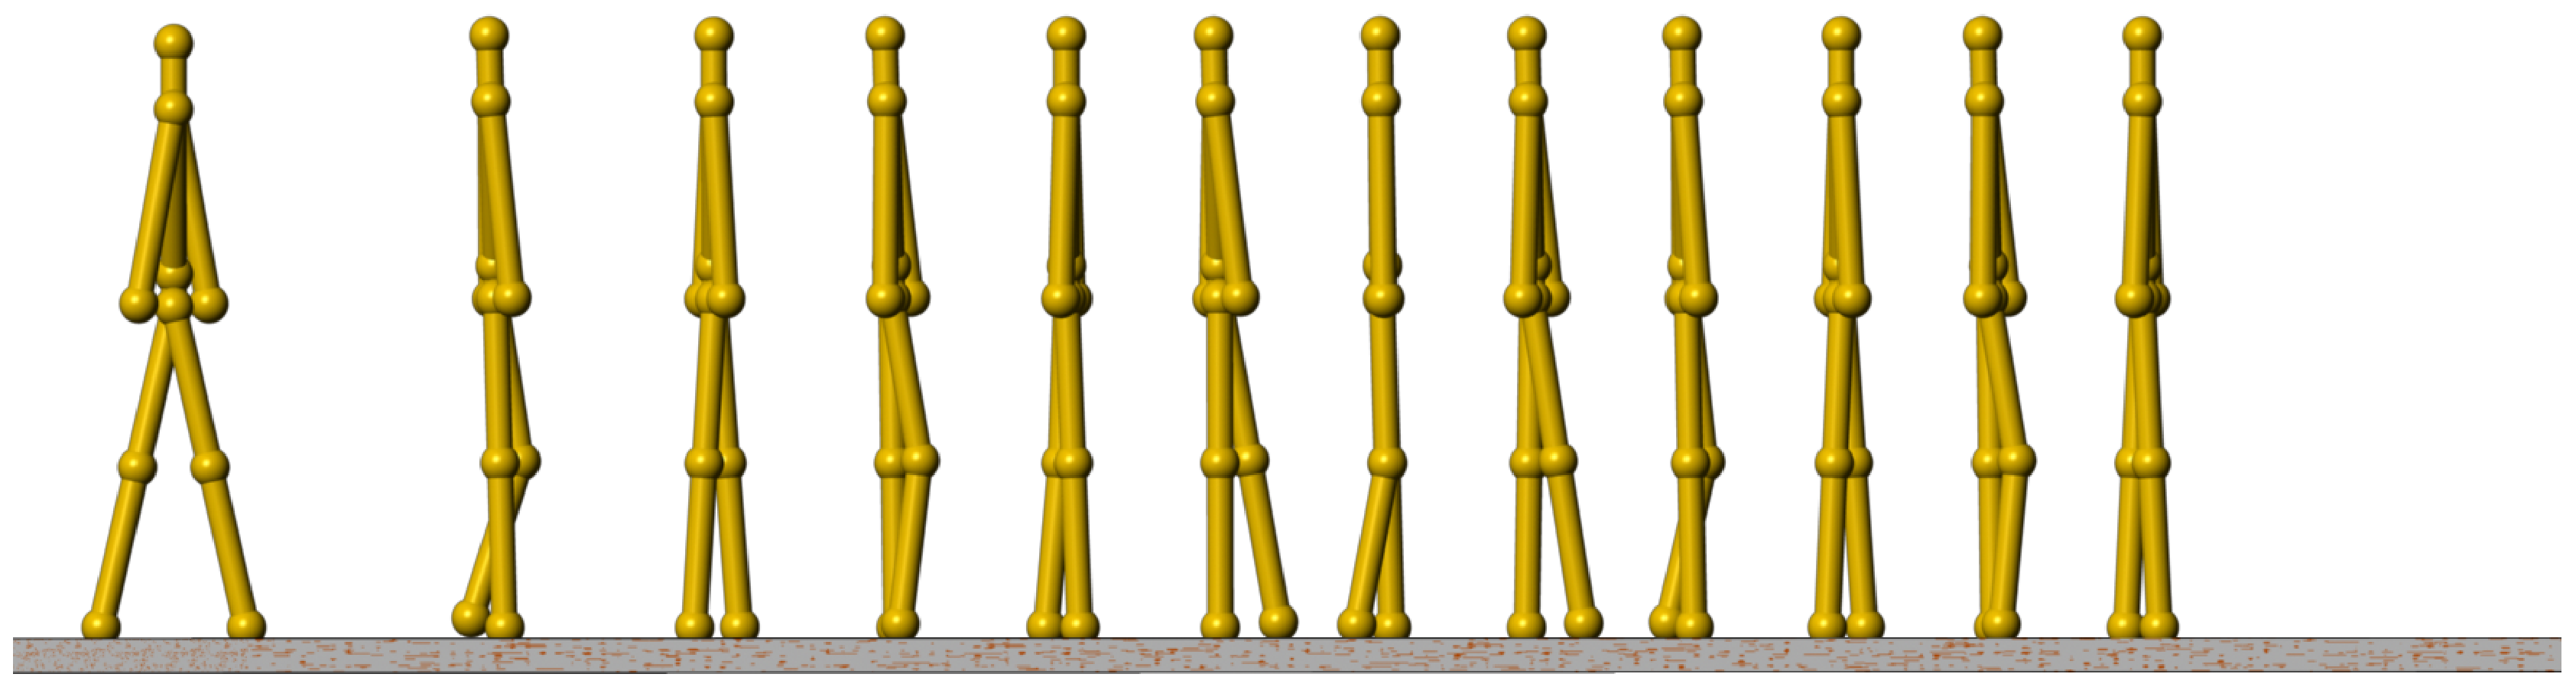
\includegraphics[width=0.7\textwidth]{walking_with_neural}
    \caption{Place Holder2}
    \label{fig:ss2}
\end{center}
\end{figure}

\begin{figure}[!htbp]
  \begin{center}
      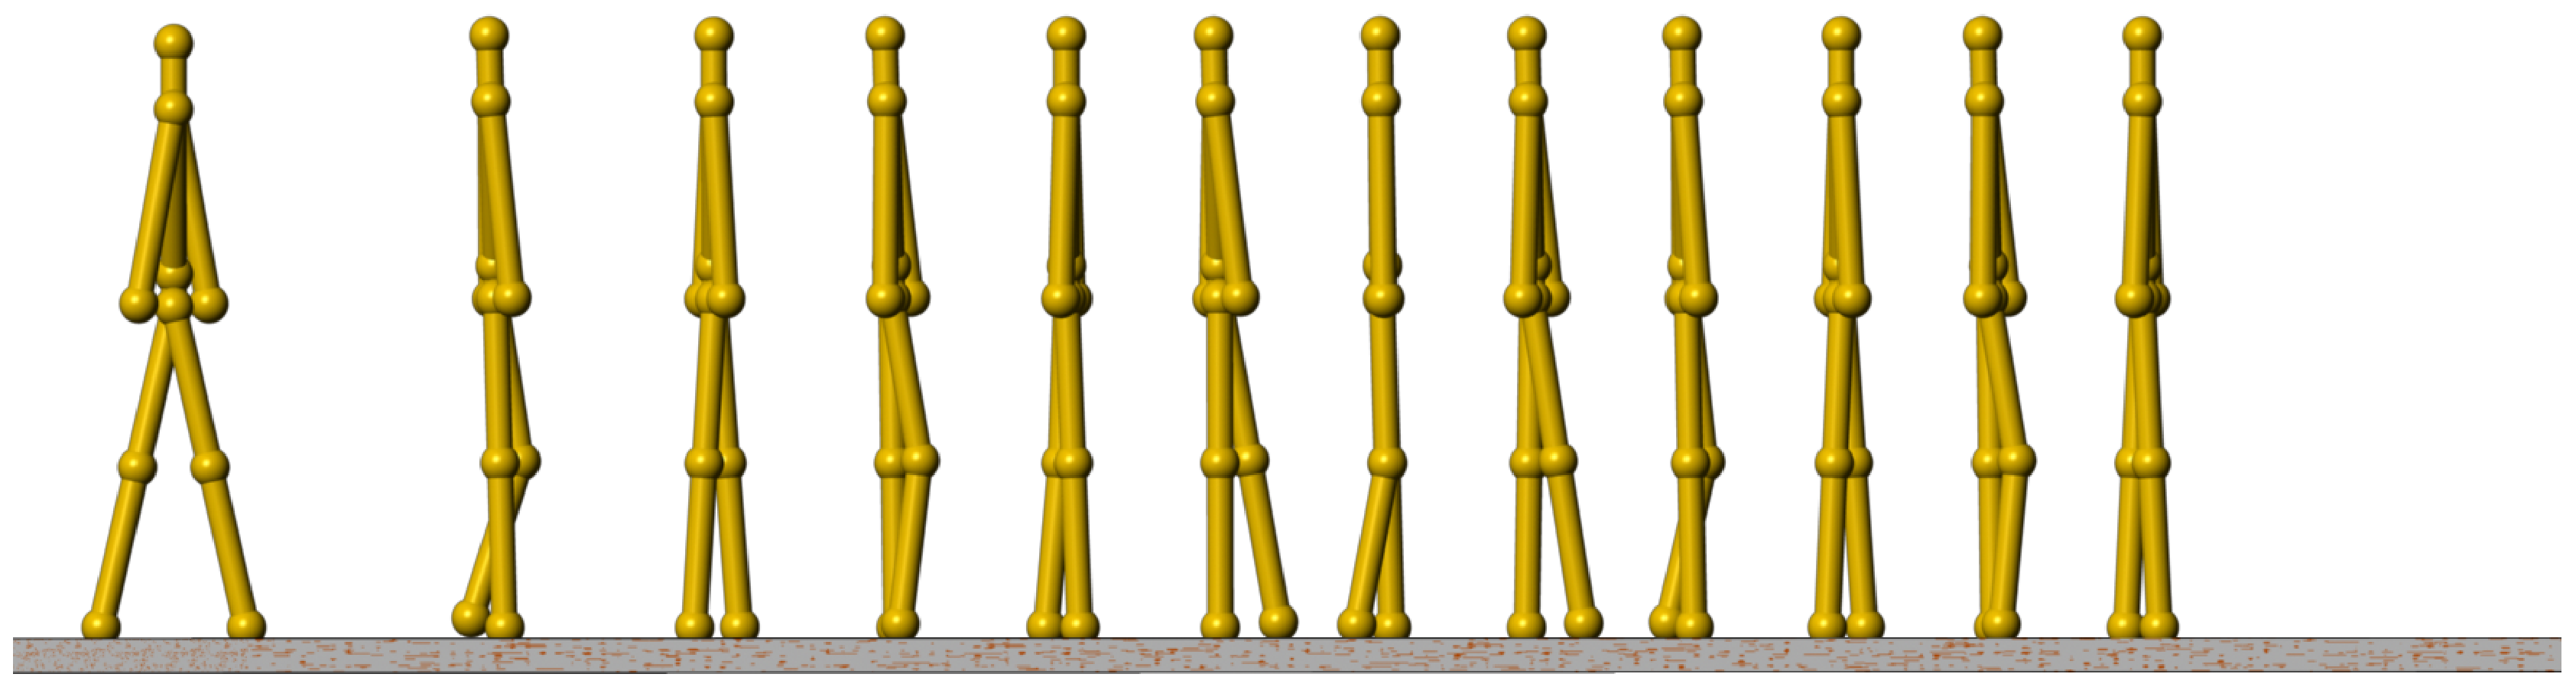
\includegraphics[width=0.7\textwidth]{walking_with_neural}
    \caption{Place Holder3}
    \label{fig:ss3}
\end{center}
\end{figure}




\subsubsection*{Different Leg Mass}
we also change the leg mass of the two leggs, make them not equal.
This will result two legs sway differently and the limit circle of orignal system is doubled.
Bigger difference will result in a gait looks like cripple.

\begin{figure}[!htbp]
  \begin{center}
    \leavevmode
    \ifpdf
      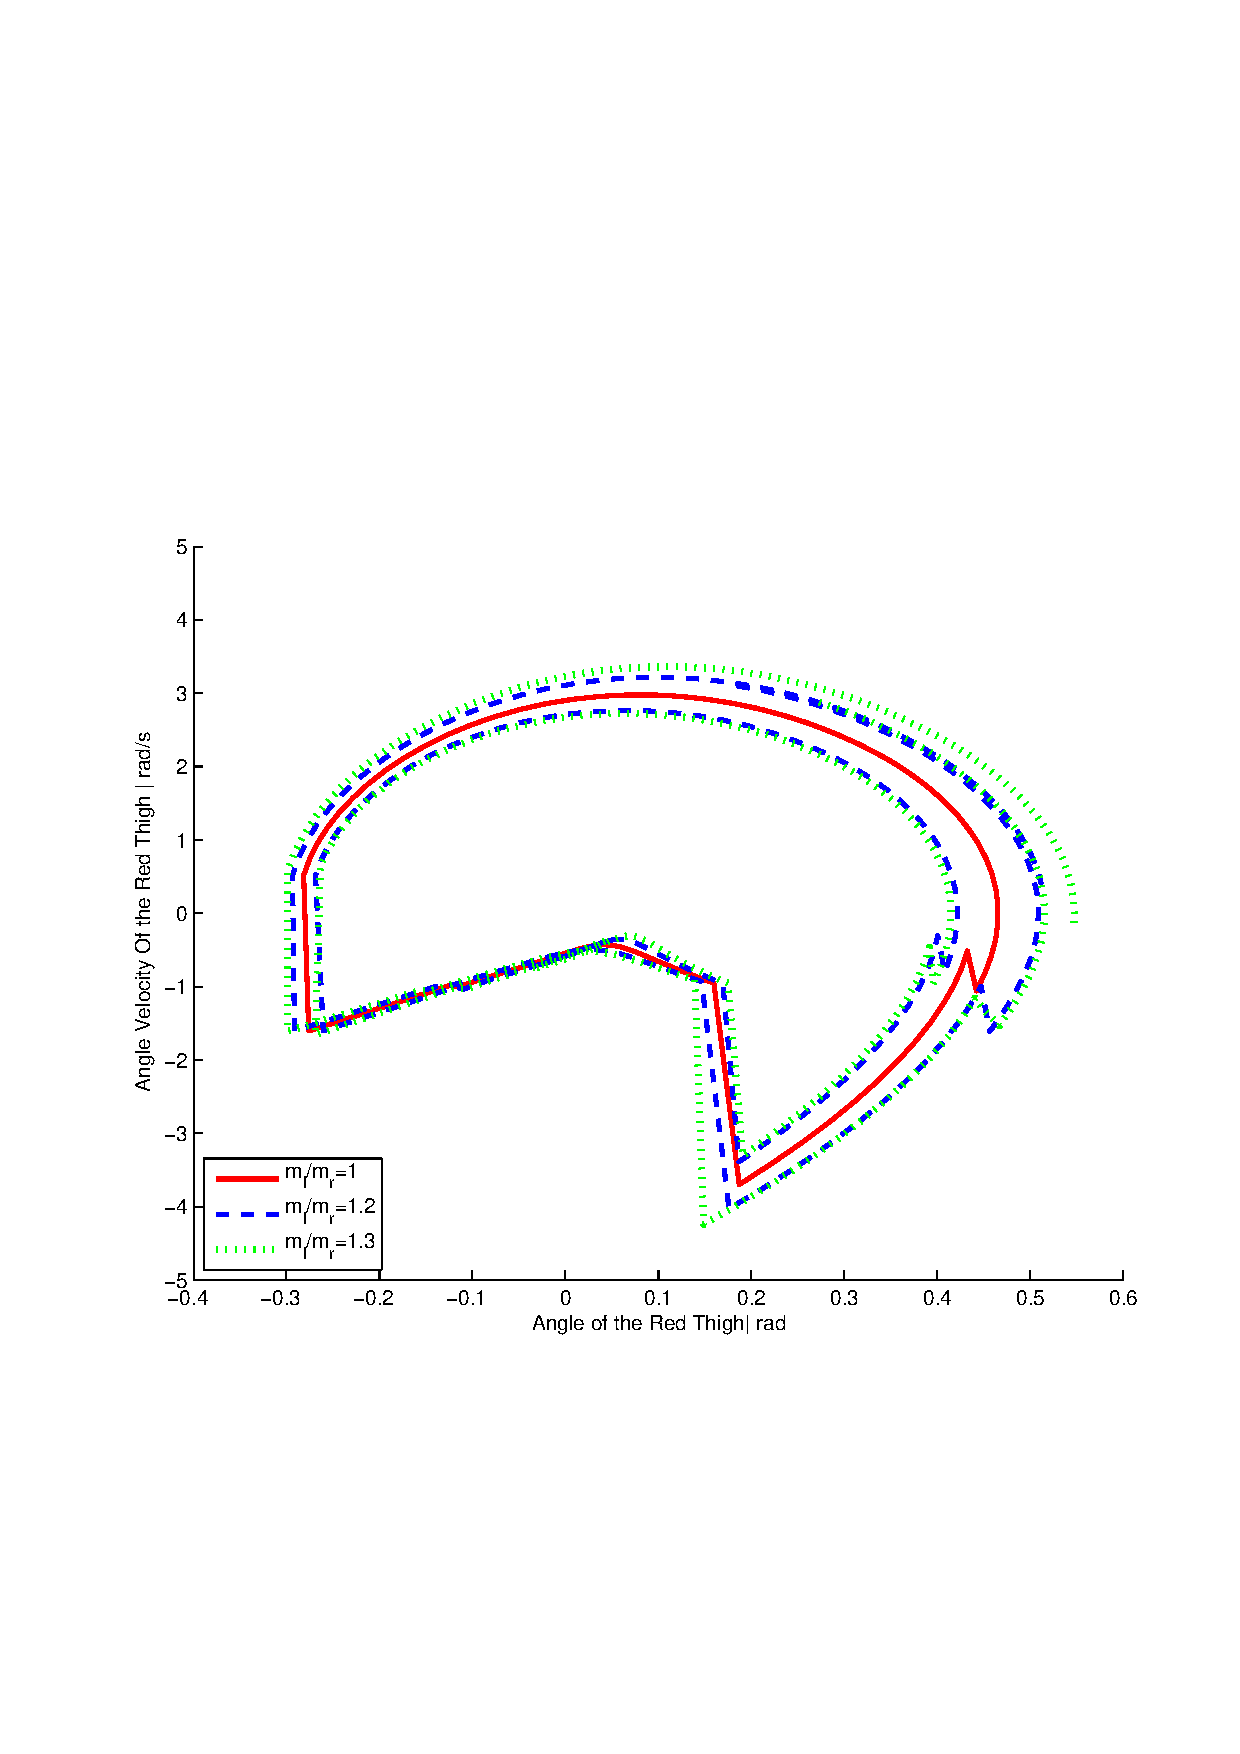
\includegraphics[height=6in]{DifferentLegMassLimitCircle}
    \else
      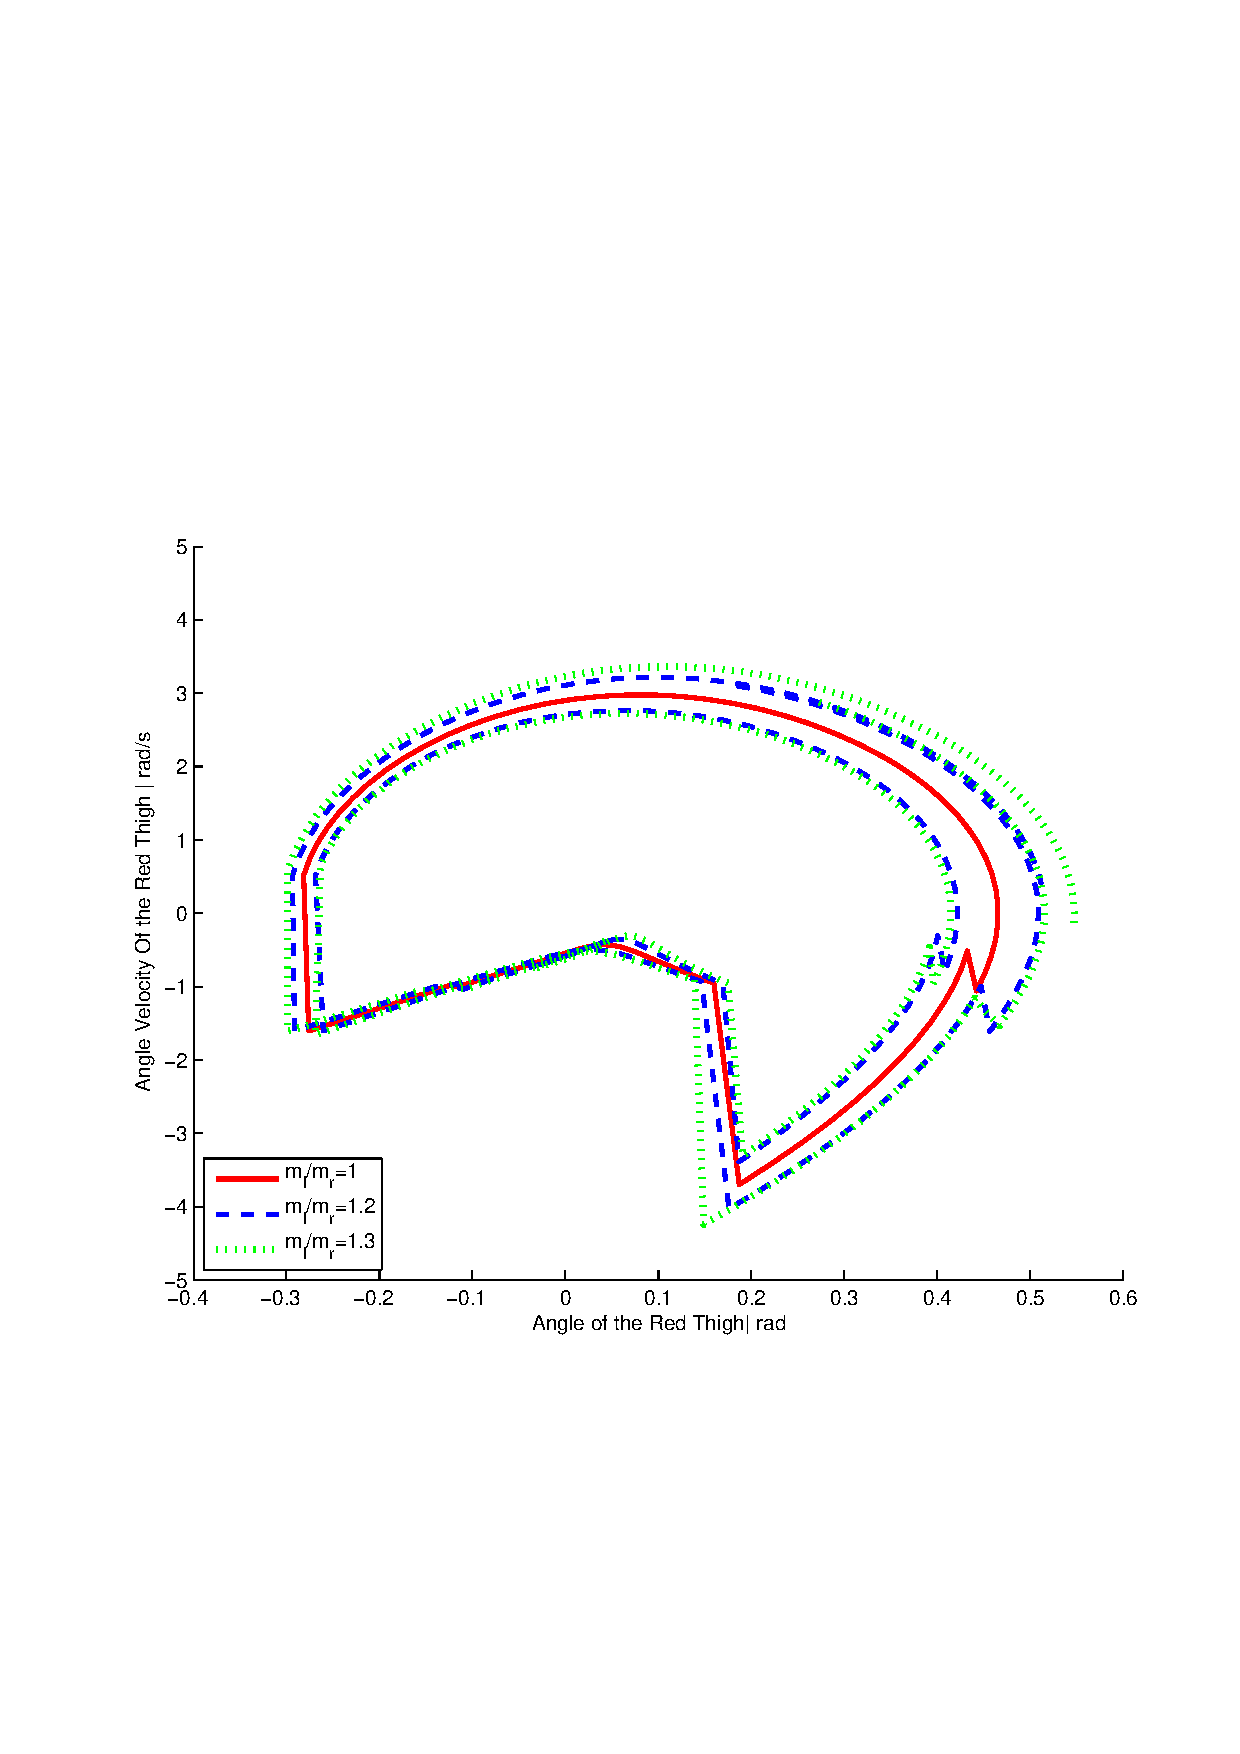
\includegraphics[width=0.7\textwidth]{DifferentLegMassLimitCircle}
    \fi
    \caption{Different Leg Mass Stable Gaits}
    \label{fig:differentlr}
\end{center}
\end{figure}


\begin{figure}[!htbp]
  \begin{center}
      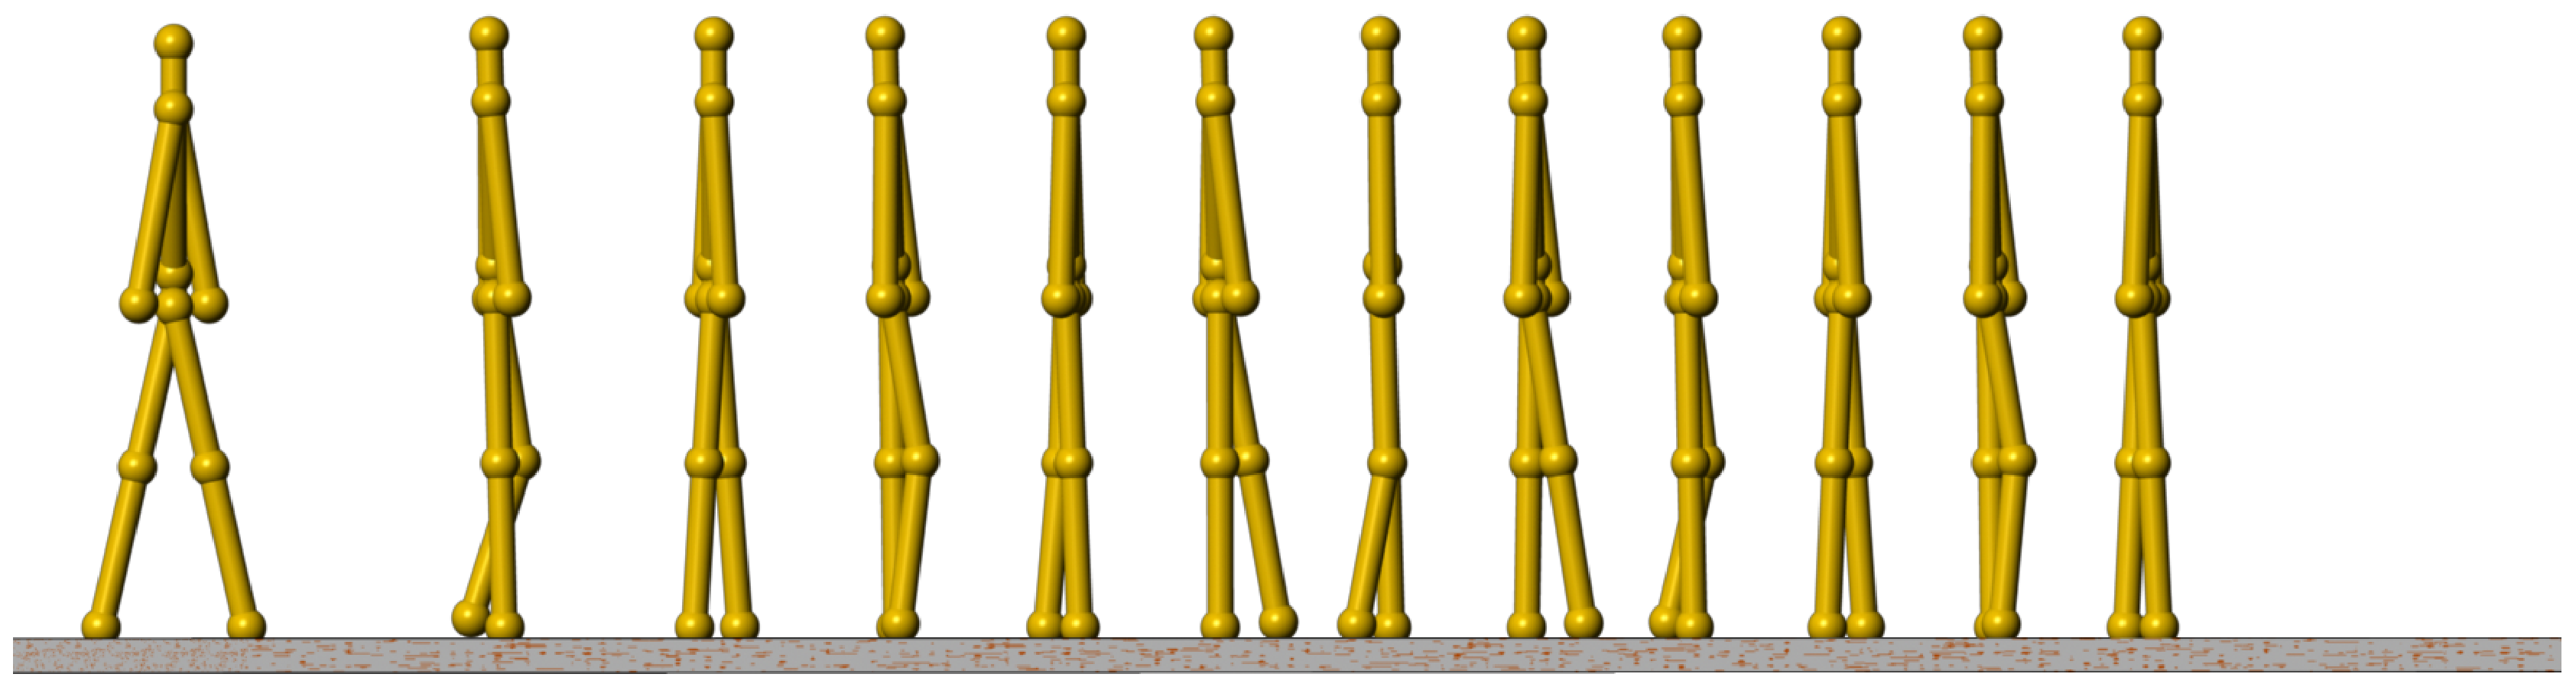
\includegraphics[width=0.7\textwidth]{walking_with_neural}
    \caption{Place Holder1}
    \label{fig:lm1}
\end{center}
\end{figure}

\begin{figure}[!htbp]
  \begin{center}
      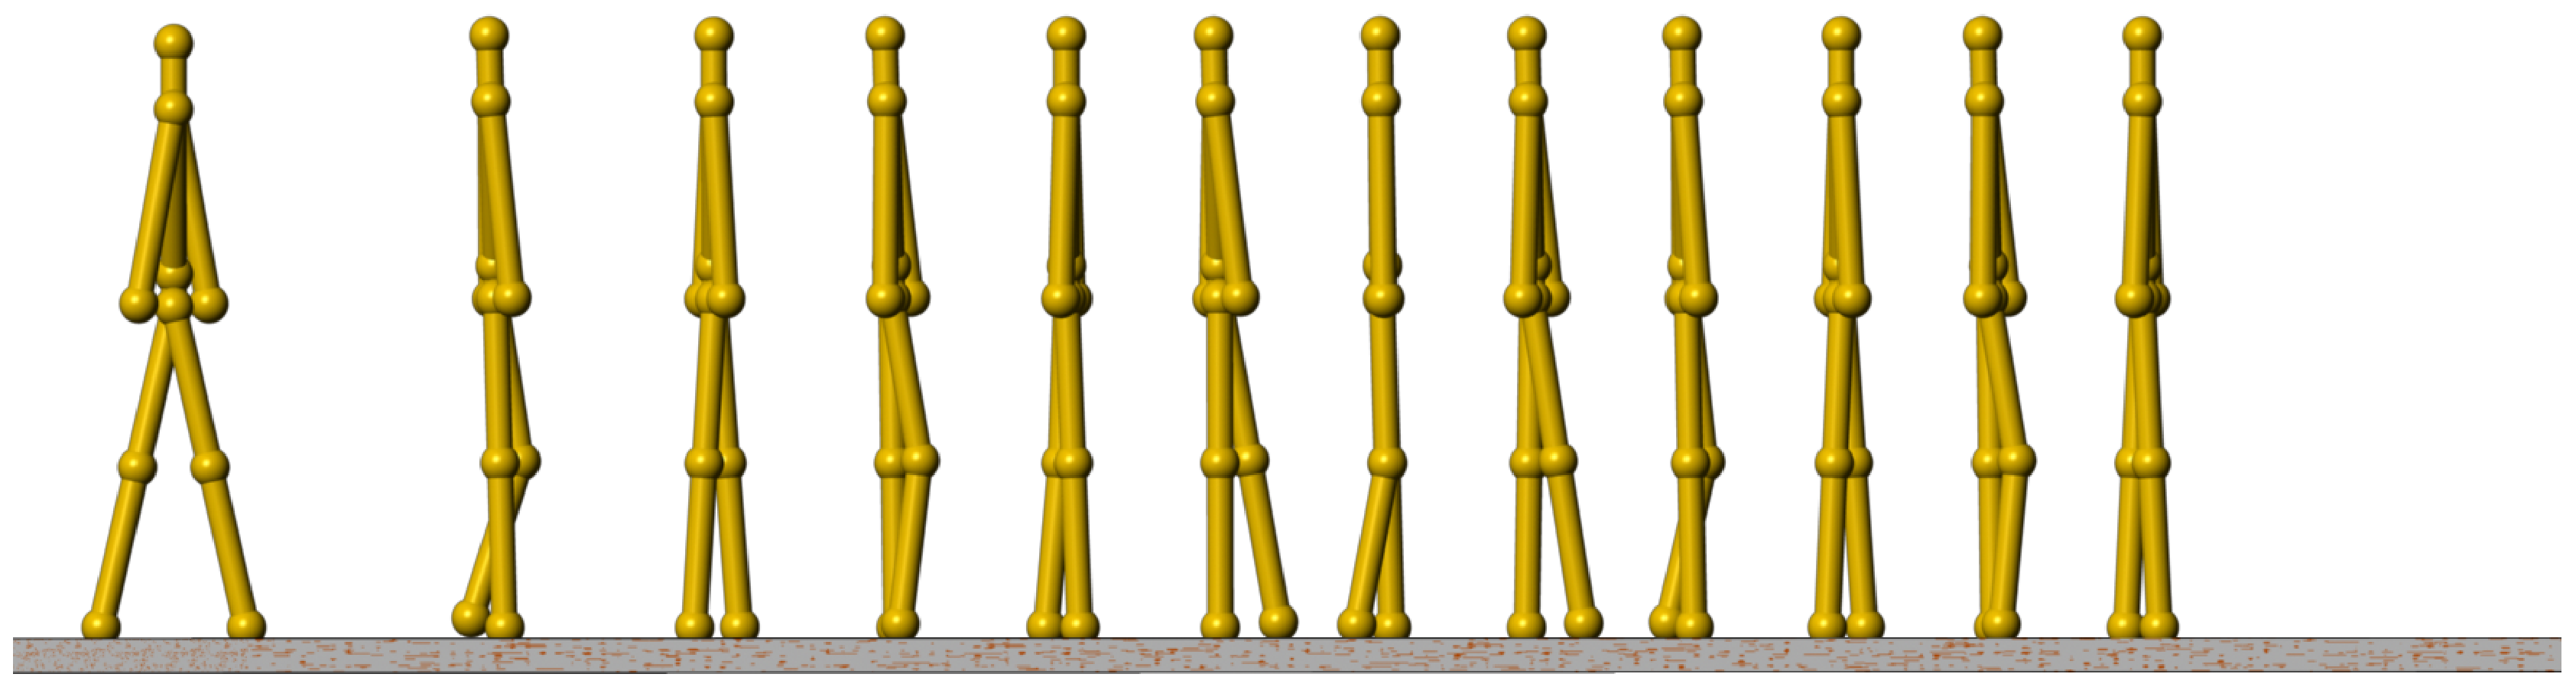
\includegraphics[width=0.7\textwidth]{walking_with_neural}
    \caption{Place Holder2}
    \label{fig:lm2}
\end{center}
\end{figure}

\begin{figure}[!htbp]
  \begin{center}
      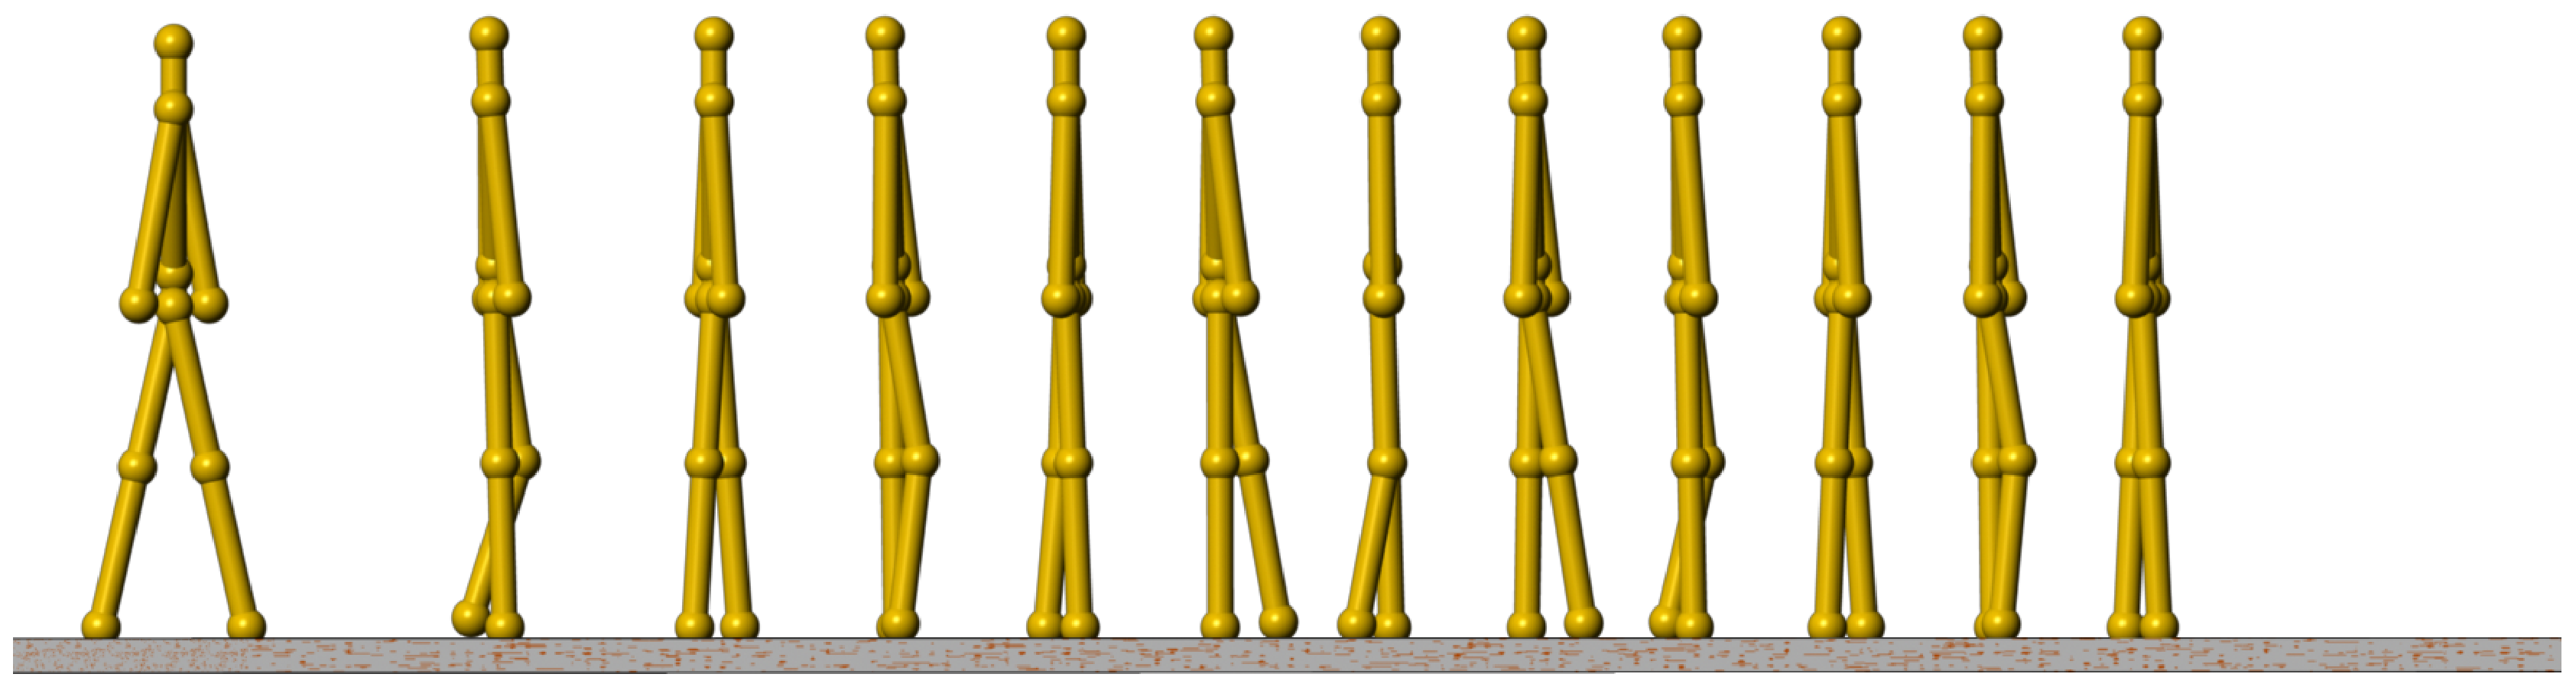
\includegraphics[width=0.7\textwidth]{walking_with_neural}
    \caption{Place Holder3}
    \label{fig:lm3}
\end{center}
\end{figure}


%lmass/rmass=1

%lmass/rmass=0.75


the period is double and the step is not symmetrical any more. So the two legs move in a slight different manner, but still, it keeps walking.

\section{Transform Gait Adaptation}
Local Invariant Controller will not generate different gait style, but it will transform the gait at different speed and at different terraint.
One important limitation we find of limit cycel is it can not walk up stope.
This is because when walking upslope, it is symmetrical to walk down the slope in another direction, if the limit cycle is stable enough, after a few steps, it will walk backwards and walk downslope.


the failure of walking up slope is show in figure

\begin{figure}[!htbp]
  \begin{center}
      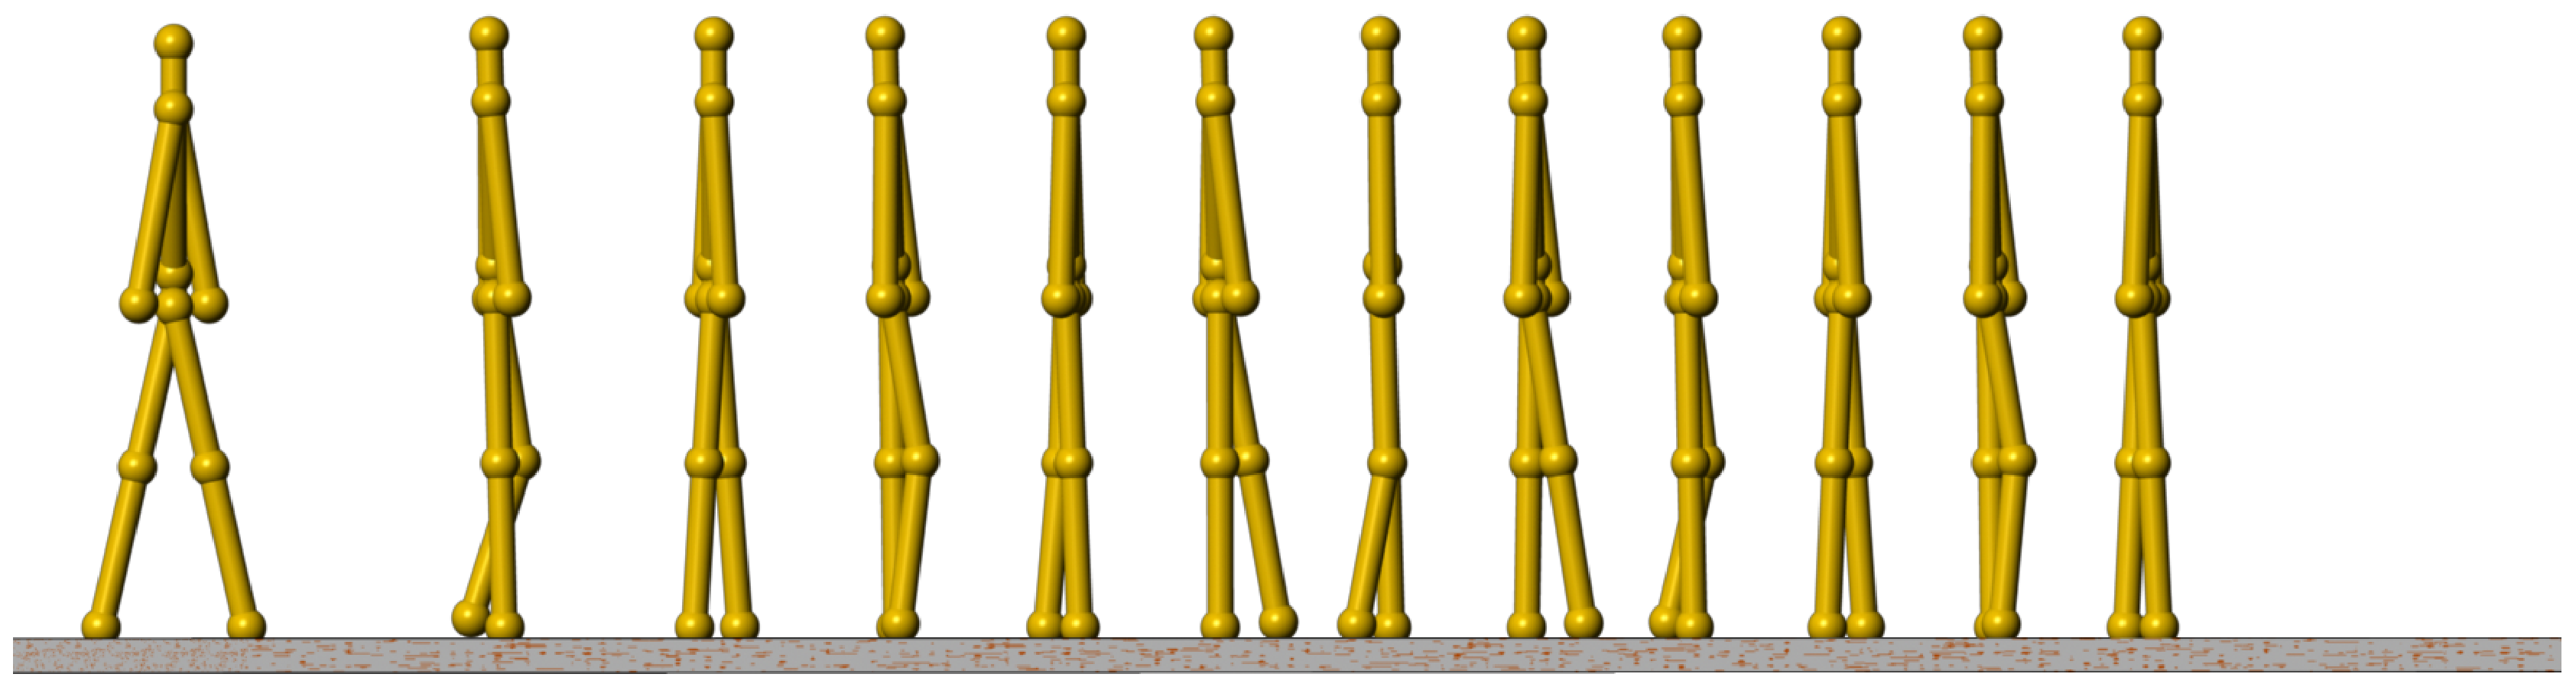
\includegraphics[width=0.7\textwidth]{walking_with_neural}
    \caption{Place Holder}
    \label{fig:withoutlocalcontroller}
\end{center}
\end{figure}

we apply two types of local motor invariant.
\begin{itemize}

\HiItem{Slope Change}.
Slope Change is incoporate through offset transformation.

%N=N*g.
\[
\ulocal=N(\mathrm{cos}(\alpha)-1)
\]
\HiItem{Speed Change}
Speed Action will ajust the walking speed, but maintain the walking gait.
the the new walking speed is $s$.
we have
\[  
\ulocal=N(\alpha^2-1)
\]
\end{itemize}

\begin{figure}[!htbp]
  \begin{center}
    \leavevmode
    \ifpdf
      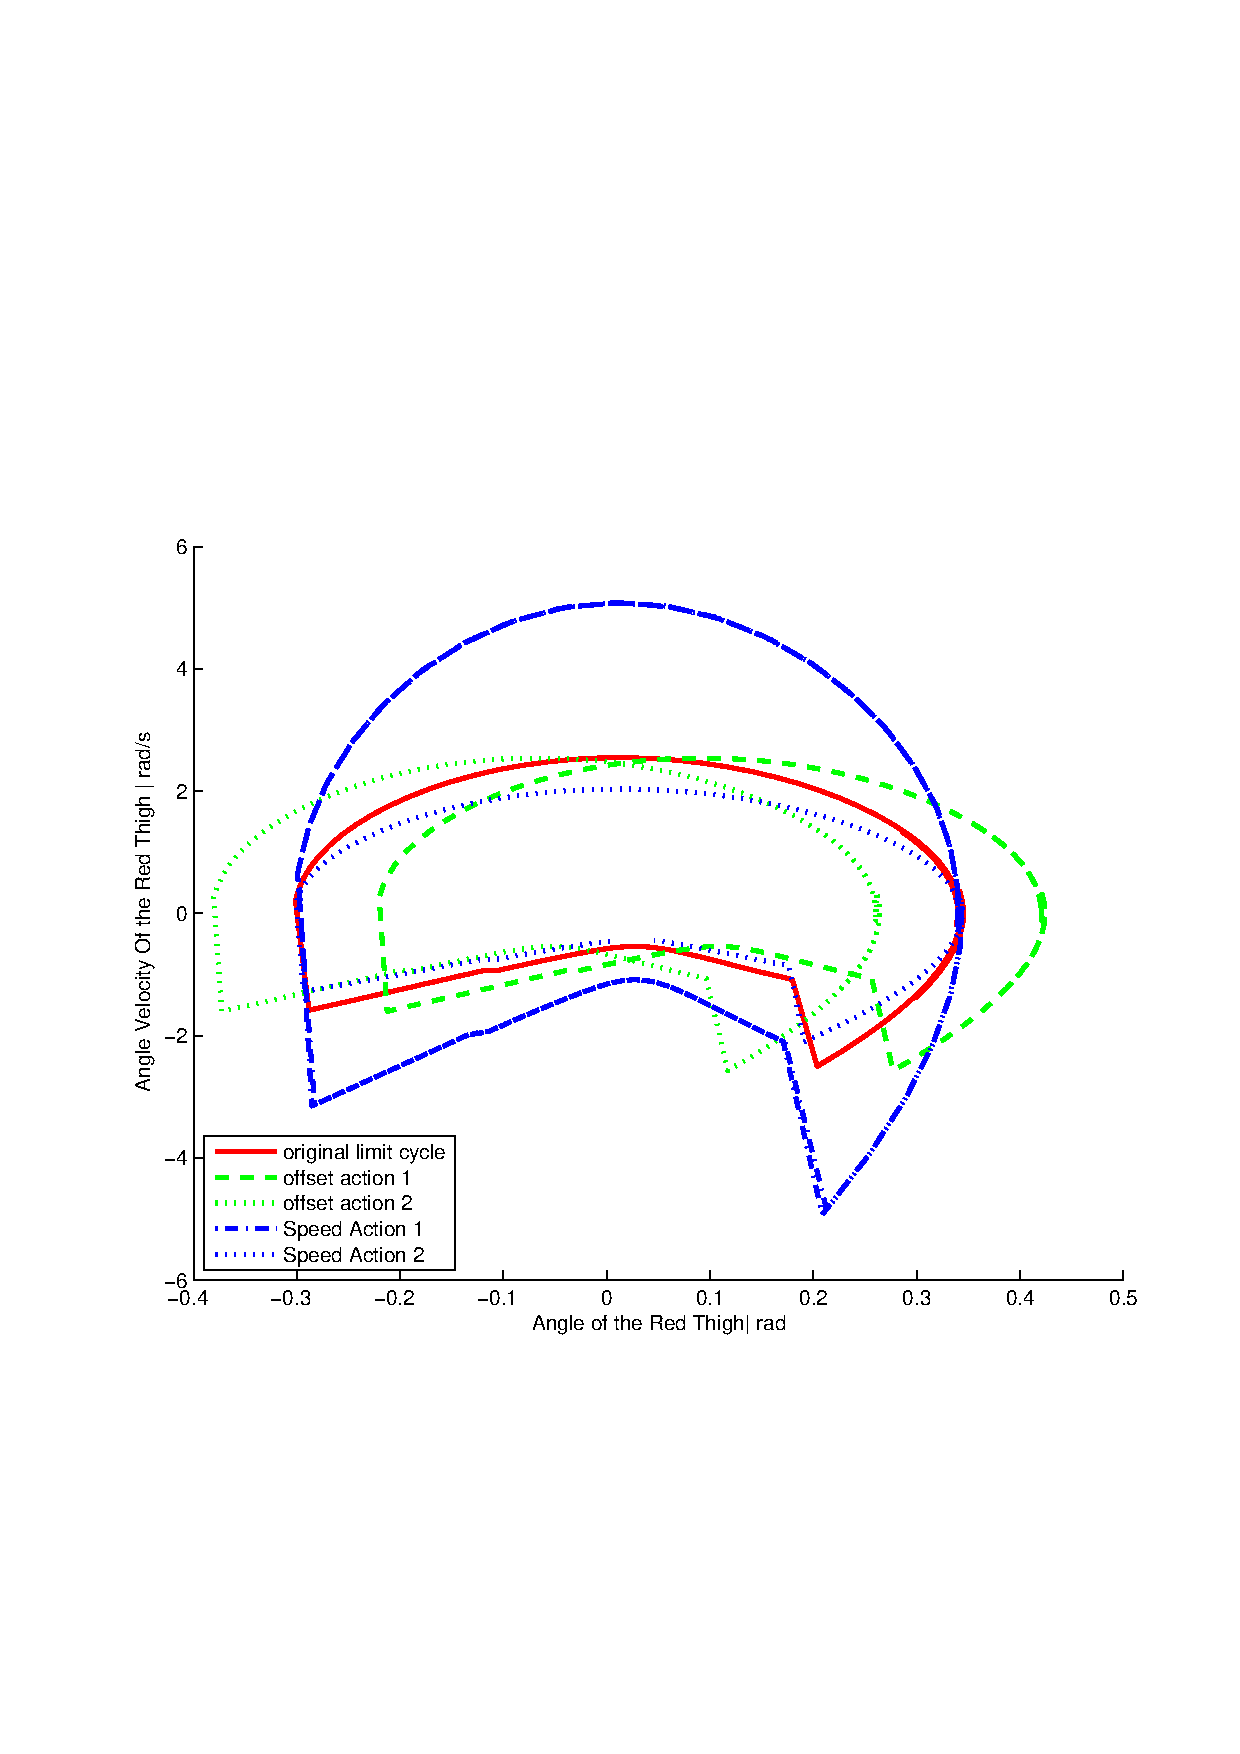
\includegraphics[height=6in]{LieGroupAction}
    \else
      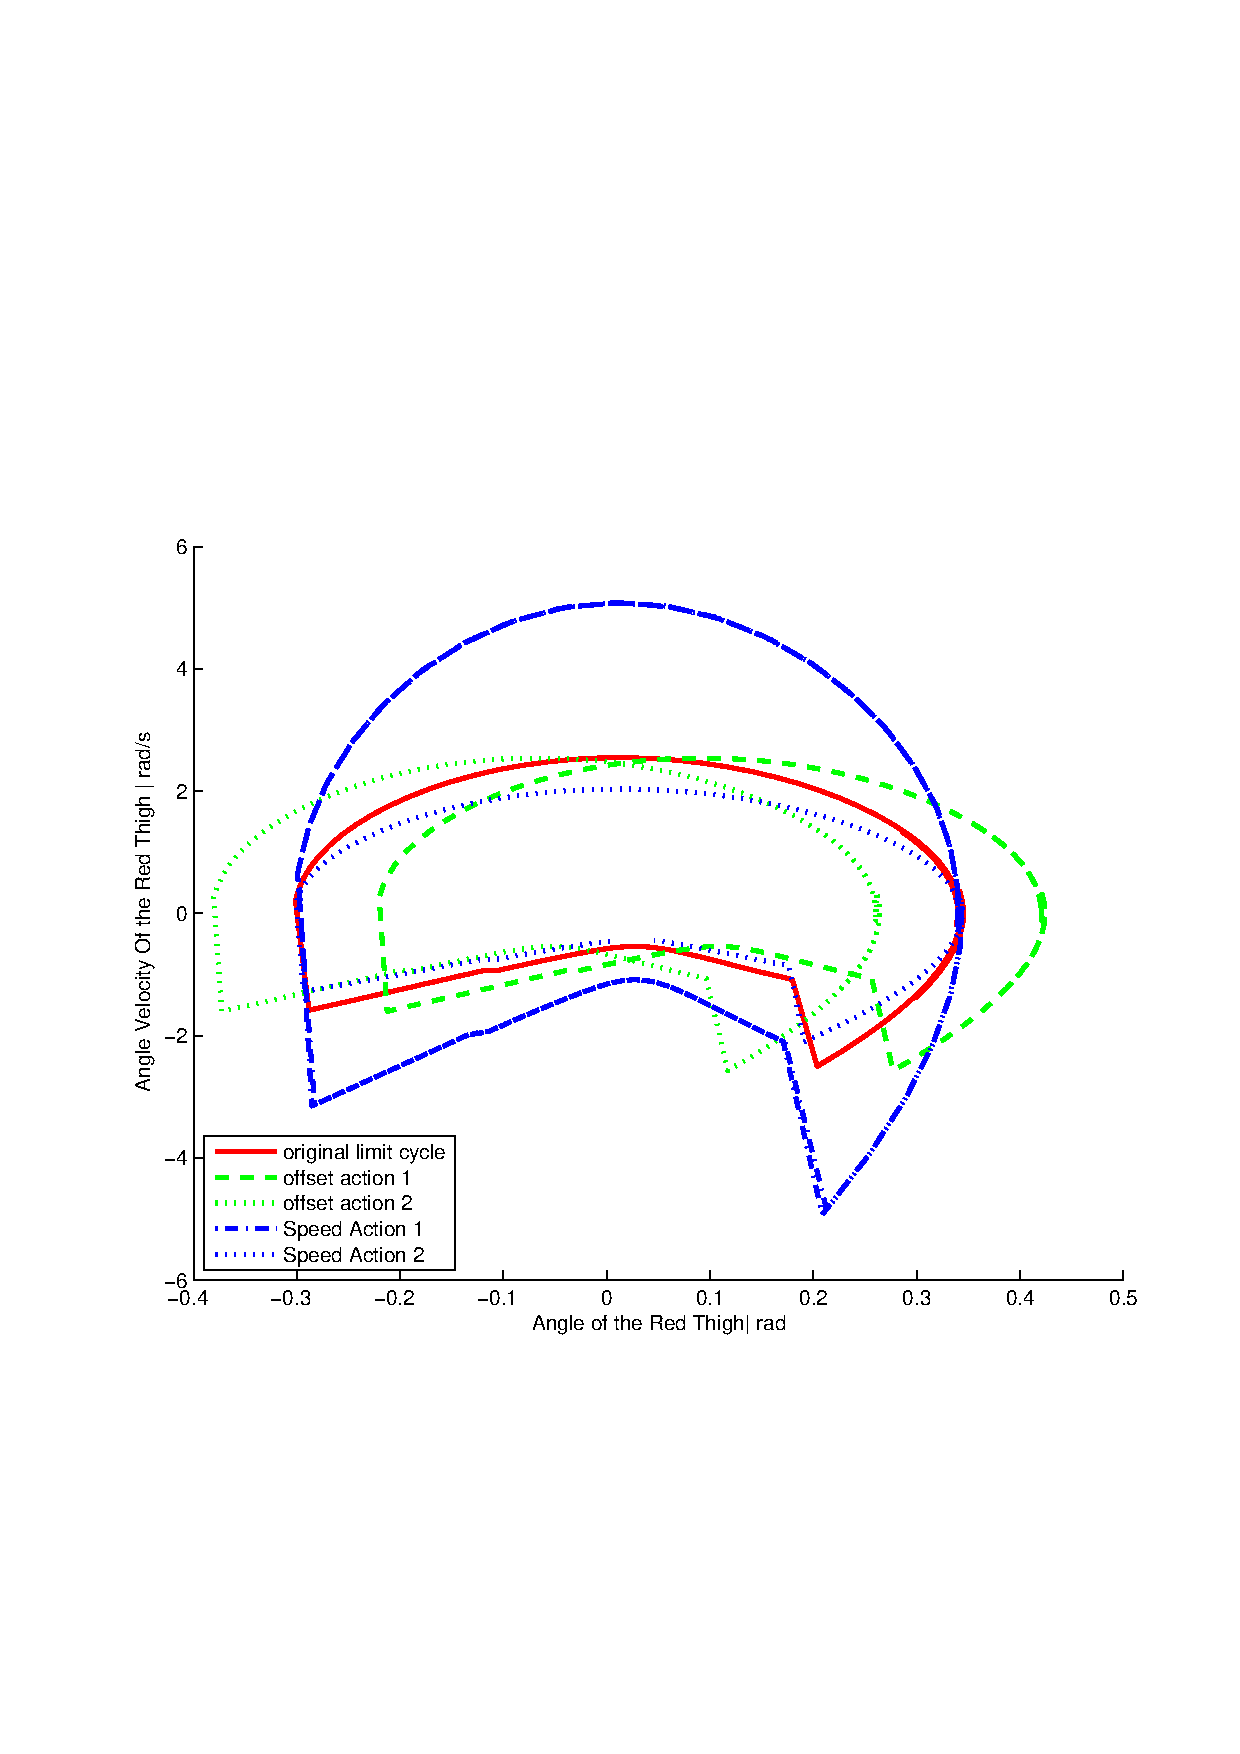
\includegraphics[width=0.7\textwidth]{LieGroupAction}
    \fi
    \caption{Different Leg Mass Stable Gaits}
    \label{fig:differentlr}
\end{center}
\end{figure}

The red on is the origianl limit cricle.
Green one are apply speed action
blueone are applied  locol stransform action

Also it can help the passive walke walk upslope.
as show in figure


\begin{figure}[!htbp]
  \begin{center}
    \leavevmode
    \ifpdf
      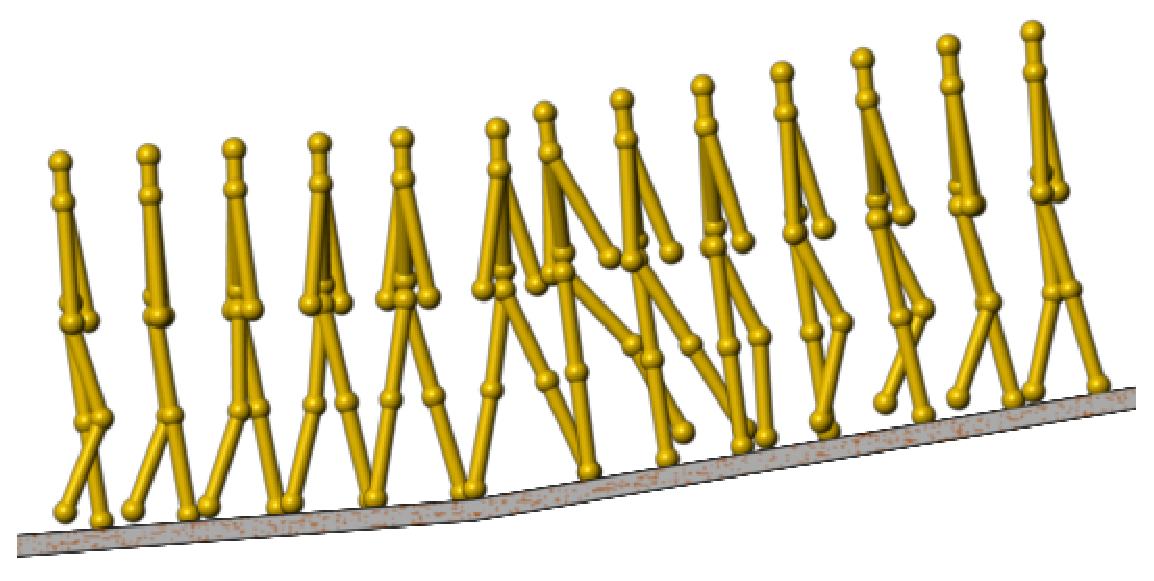
\includegraphics[height=6in]{walking_local_control}
    \else
      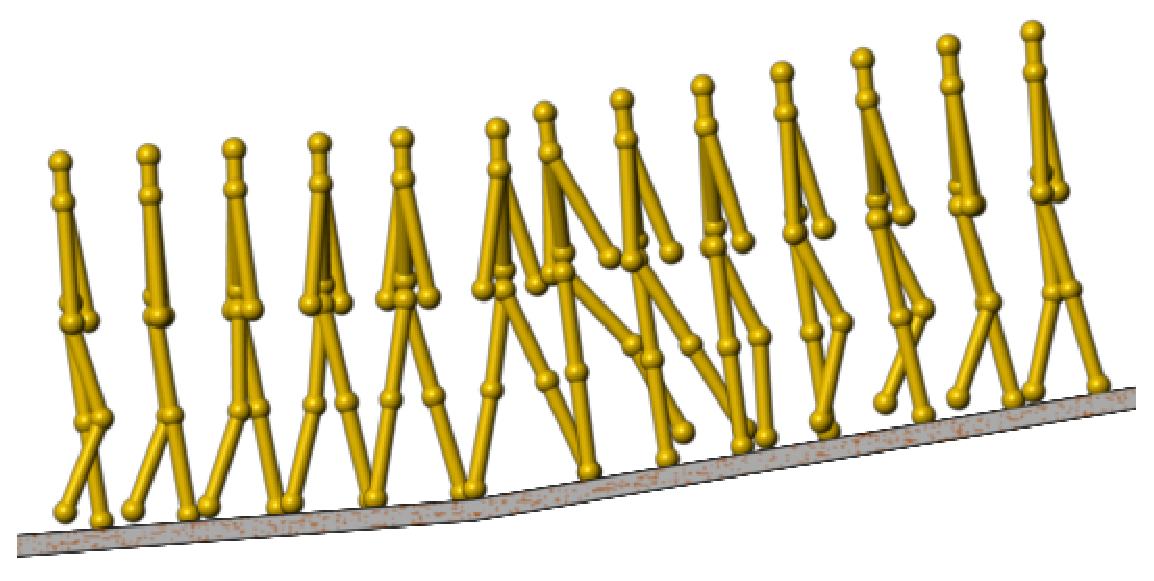
\includegraphics[width=0.7\textwidth]{walking_local_control}
    \fi
    \caption{Varying Terrain}
    \label{fig:diffterrain}
\end{center}
\end{figure}




\begin{figure}[!htbp]
  \begin{center}
    \leavevmode
    \ifpdf
      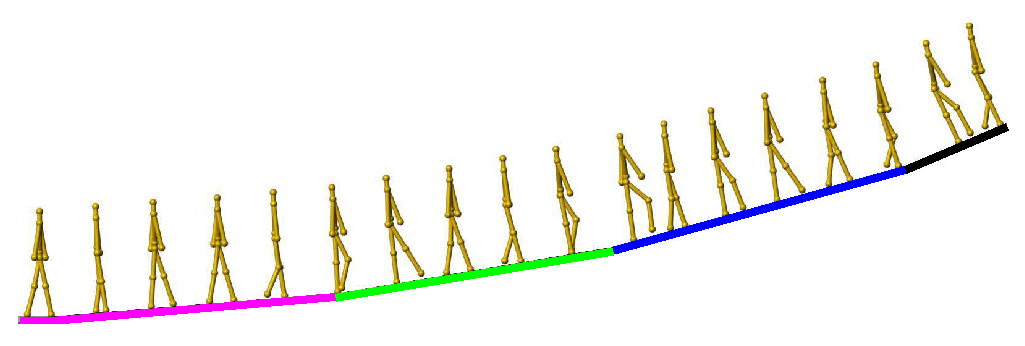
\includegraphics[height=6in]{walk_terrain_anim}
    \else
      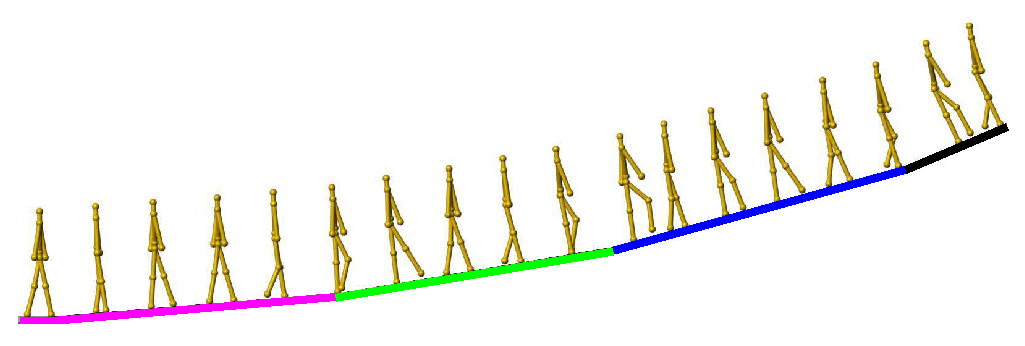
\includegraphics[width=0.7\textwidth]{walk_terrain_anim}
    \fi
    \caption{Varying Terrain}
    \label{fig:diffterrain}
\end{center}
\end{figure}



and on phase plot we see

\begin{figure}[!htbp]
  \begin{center}
    \leavevmode
    \ifpdf
      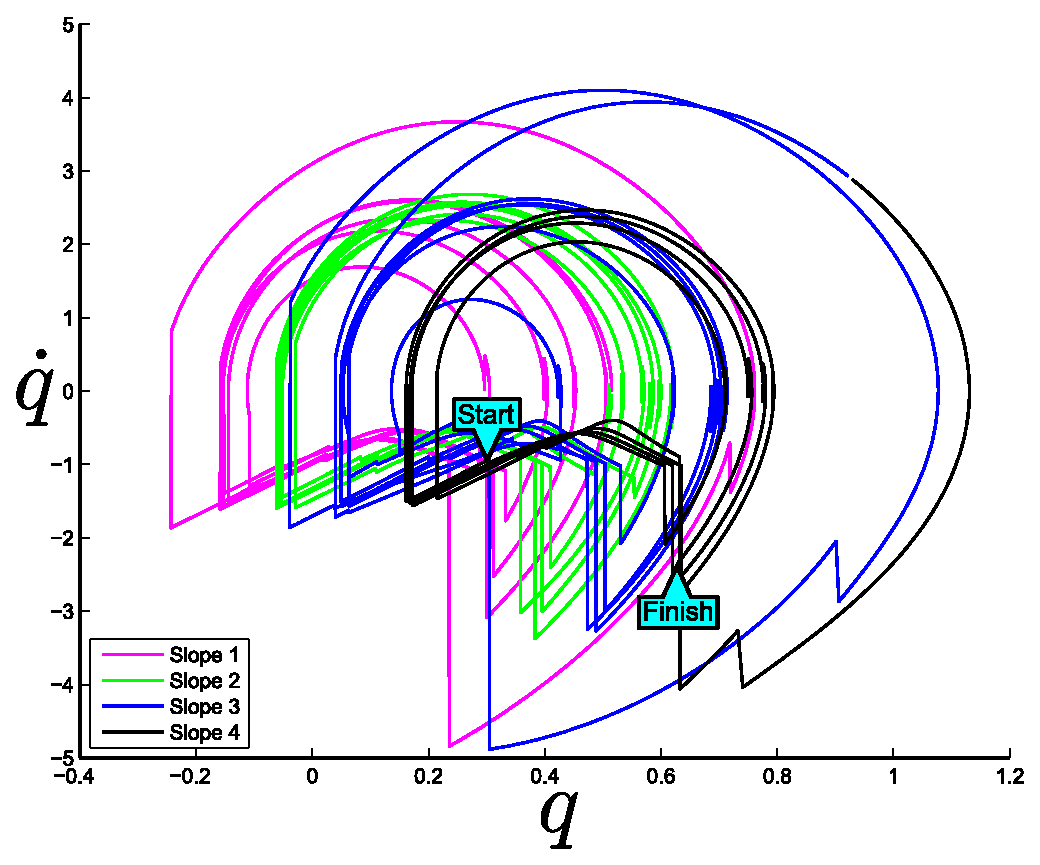
\includegraphics[height=6in]{walk_terrain}
    \else
      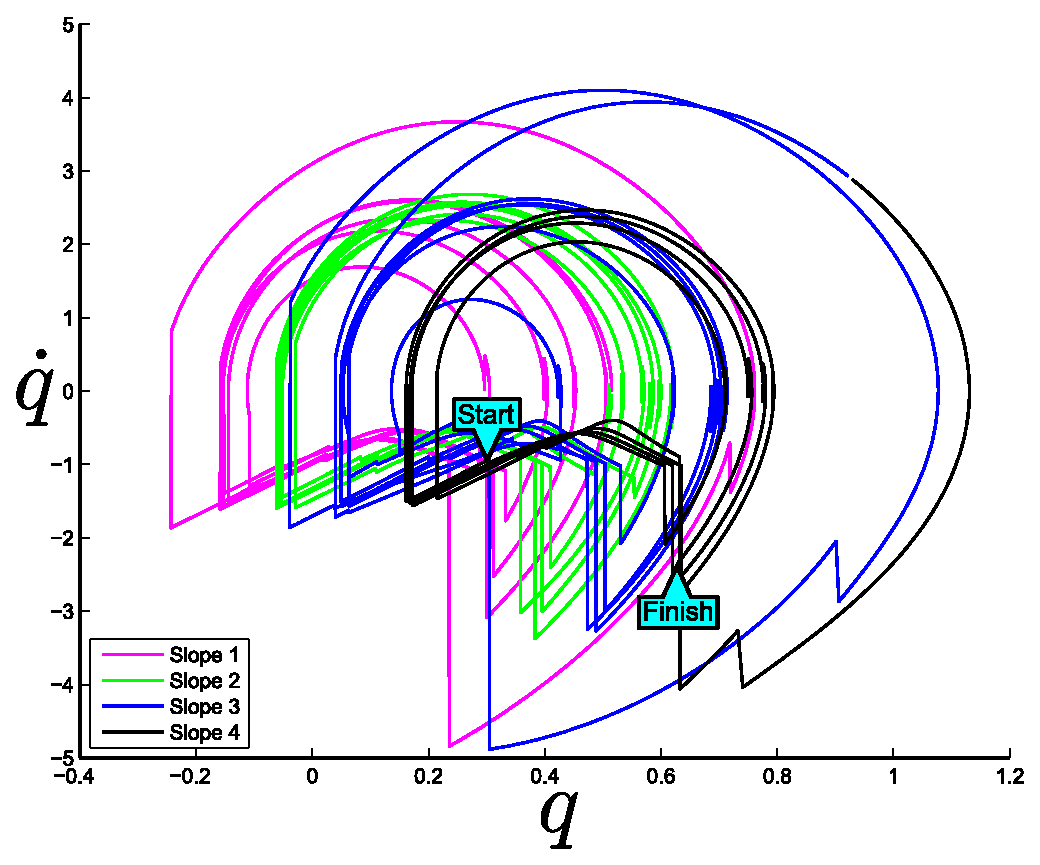
\includegraphics[width=0.7\textwidth]{walk_terrain}
    \fi
    \caption{Varying Terrain}
    \label{fig:diffterrainphase}
\end{center}
\end{figure}

and another terrain.
\begin{figure}[!htbp]
  \begin{center}
    \leavevmode
    \ifpdf
      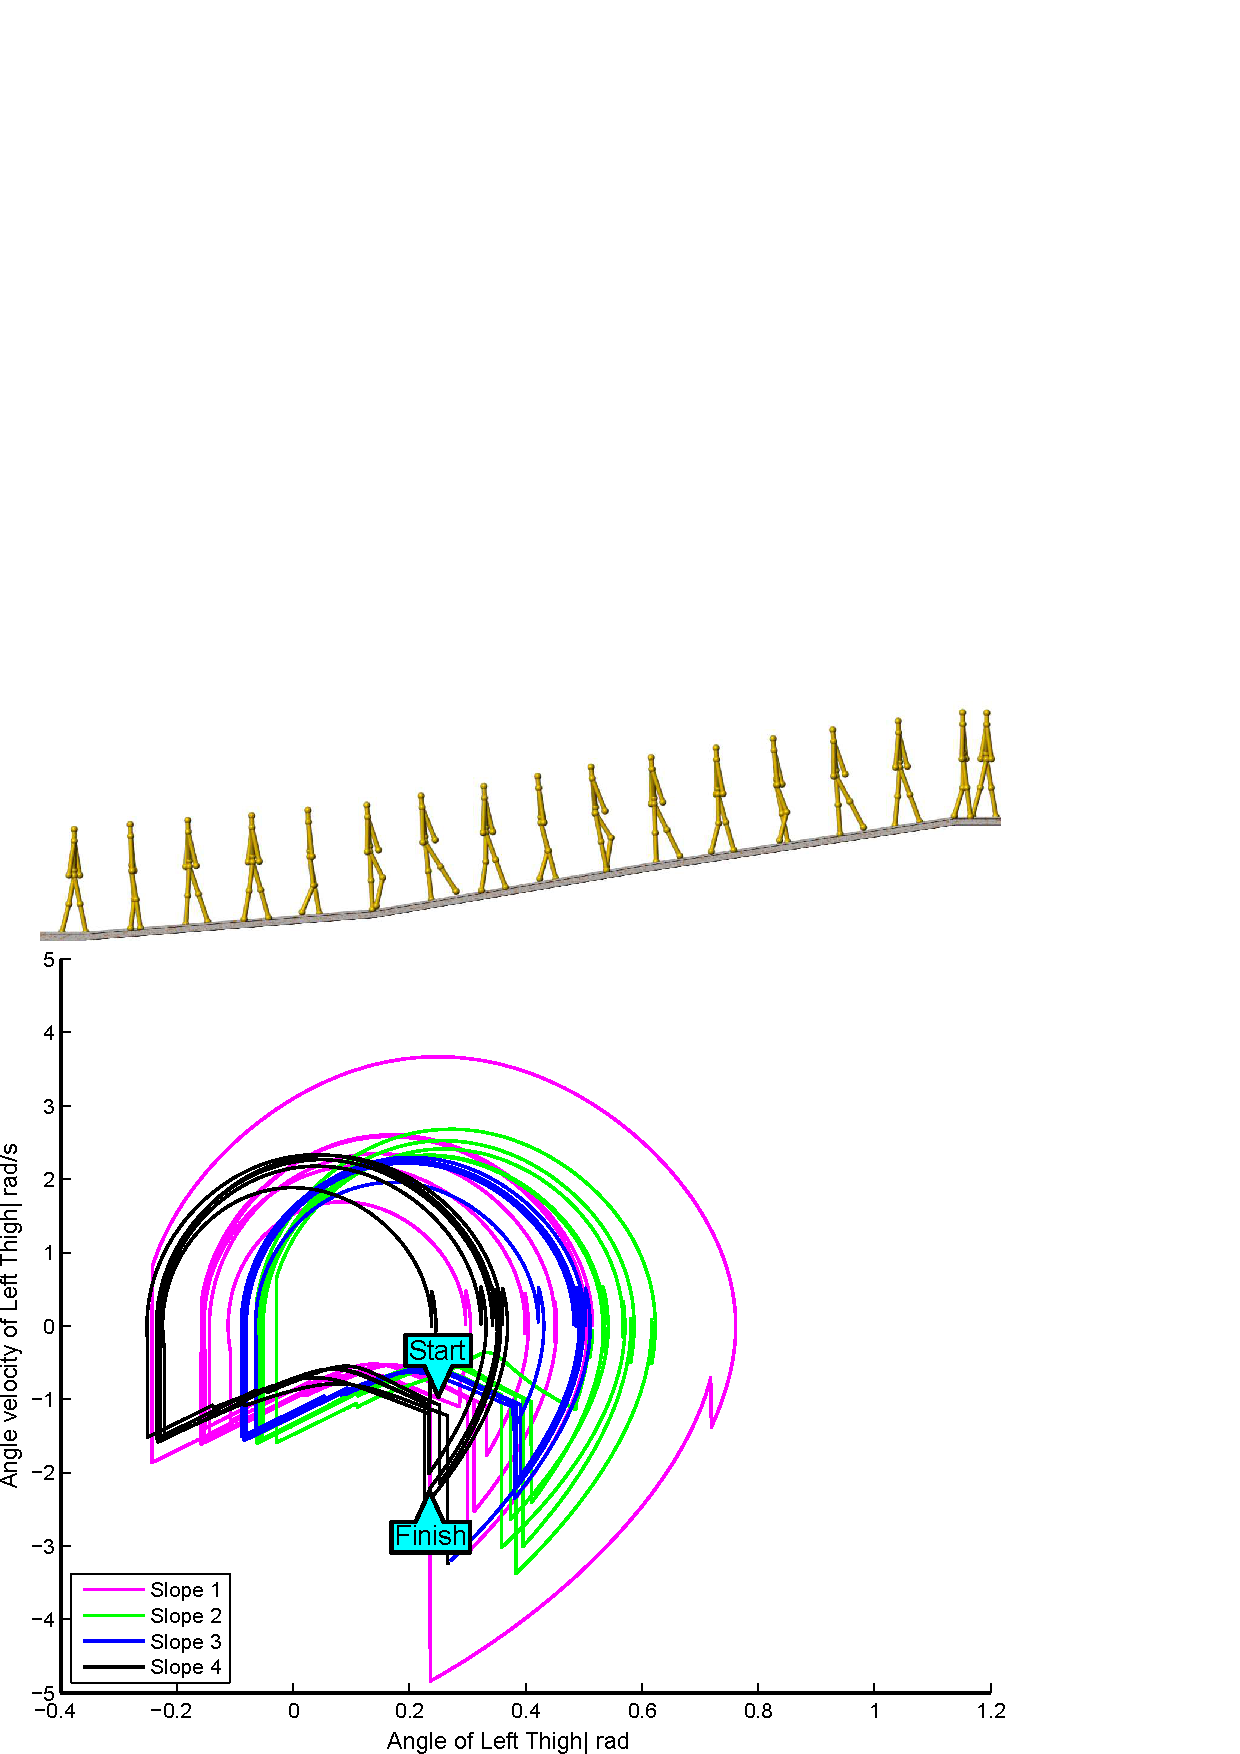
\includegraphics[height=6in]{walk_terrain2}
    \else
      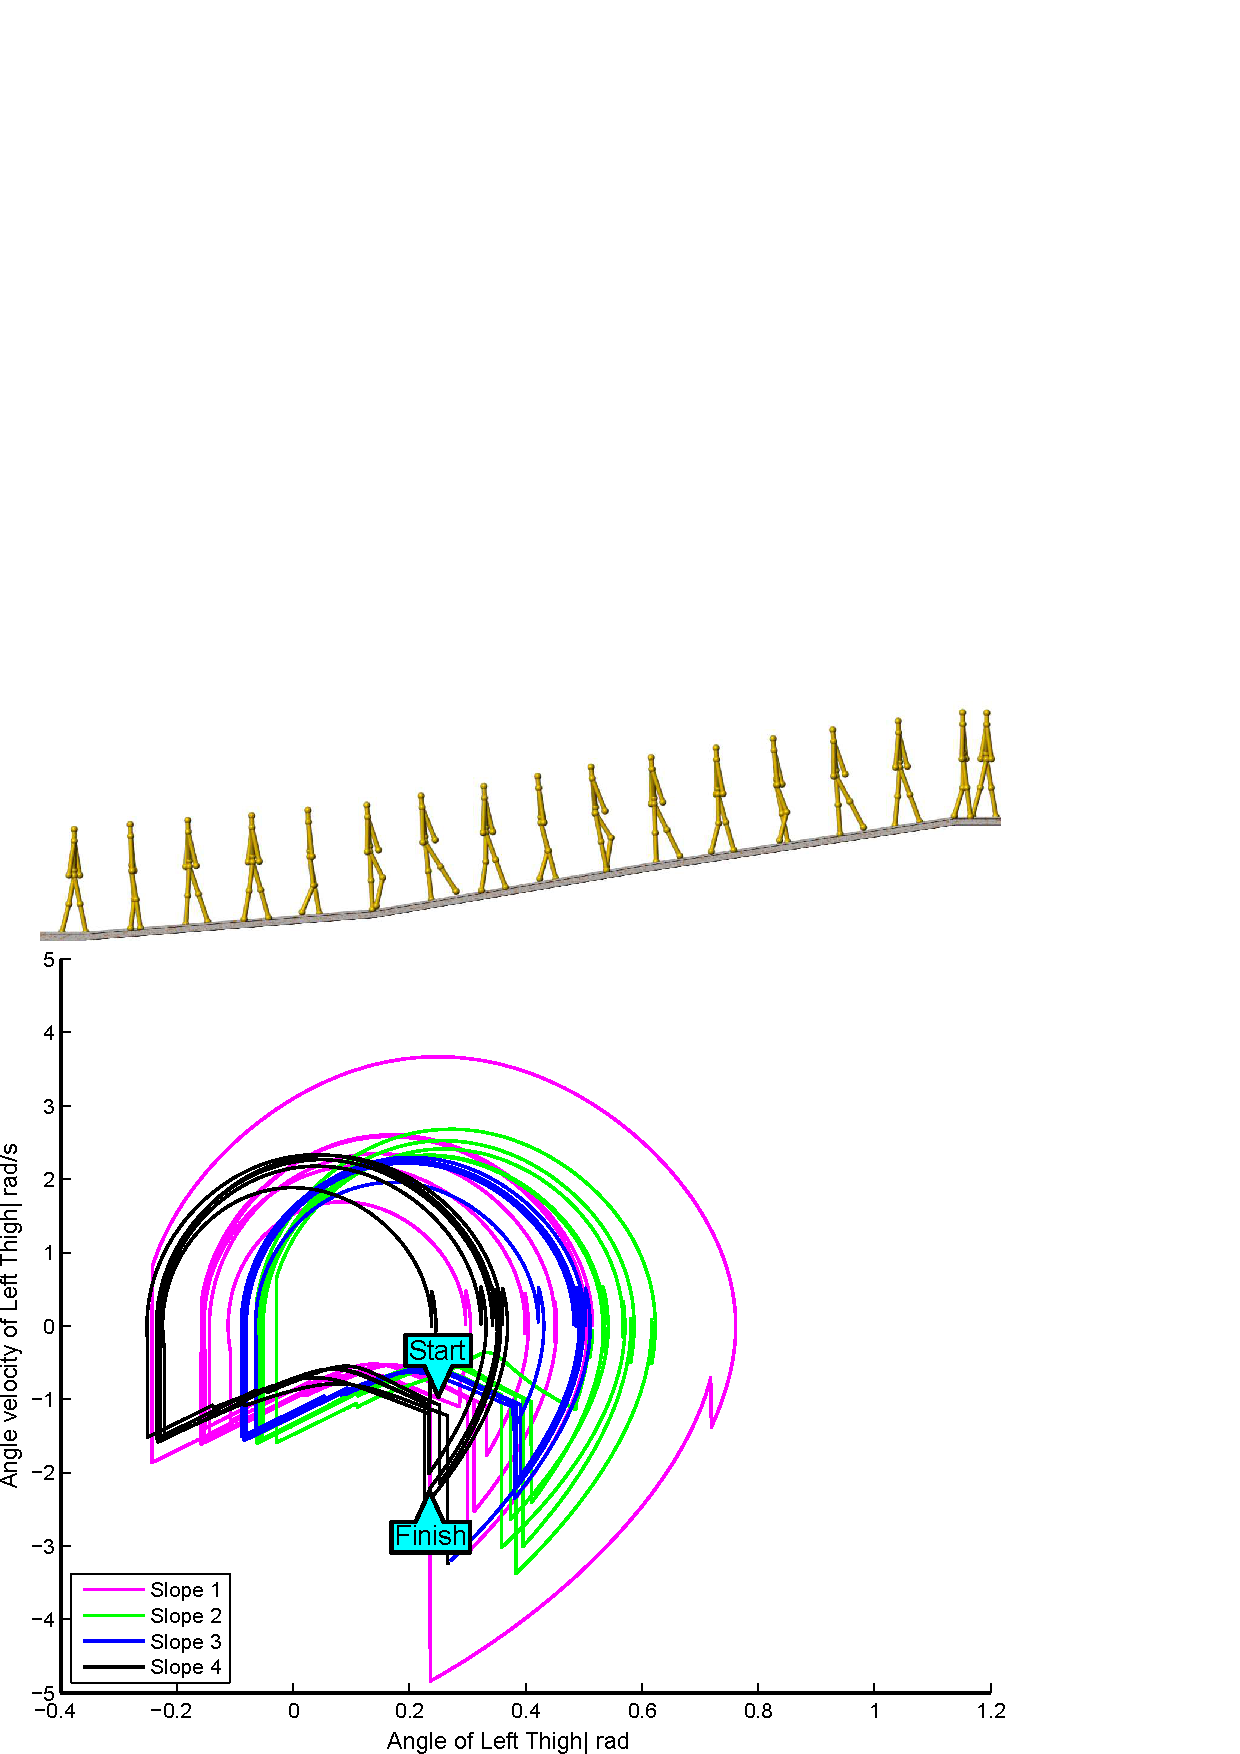
\includegraphics[width=0.7\textwidth]{walk_terrain2}
    \fi
    \caption{Varying Terrain}
    \label{fig:diffterrainphase}
\end{center}
\end{figure}


if the offset action is not enough, we find character can also walk up the slope, just with smaller step size.
Because a  smaller offset action is equalivant to walking on the same transform the gait and with the system adaption of the walking down slop.
In figure 5, we show we adjust the stepsize by changing the slope action when walking on plane.

\begin{figure}[!htbp]
  \begin{center}
      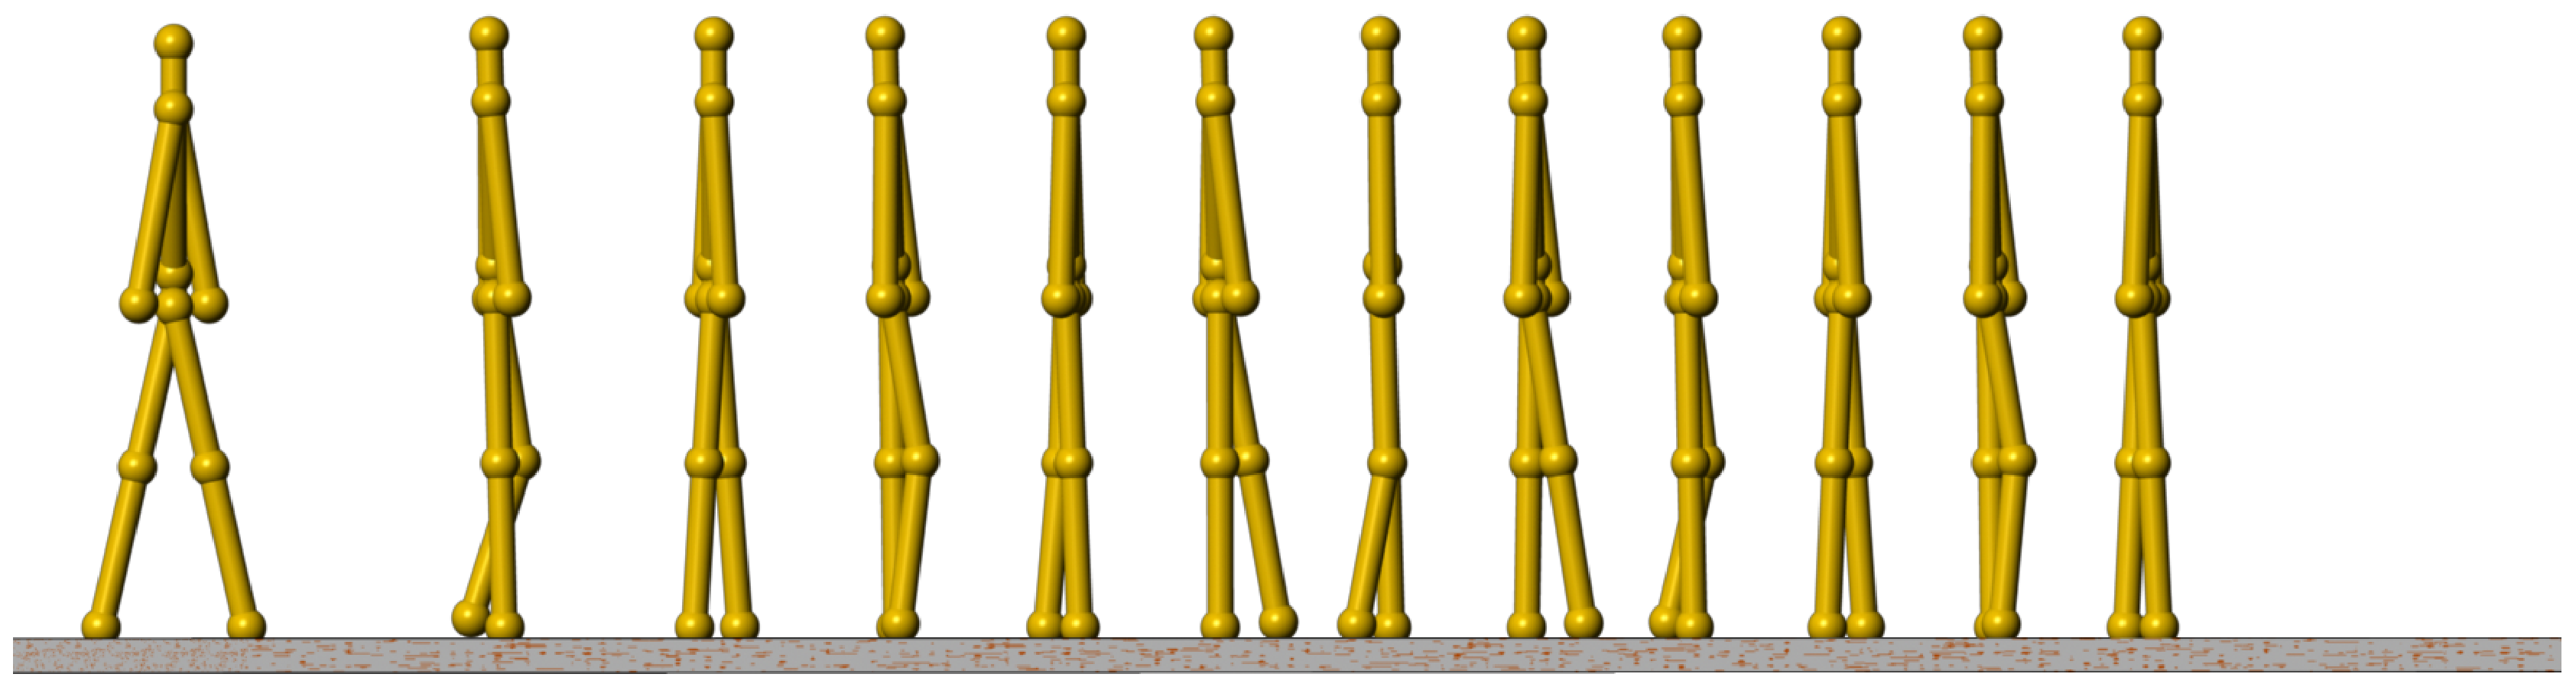
\includegraphics[width=0.7\textwidth]{walking_with_neural}
    \caption{Place Holder1}
    \label{fig:ssp1}
\end{center}
\end{figure}

\begin{figure}[!htbp]
  \begin{center}
      \includegraphics[width=0.7\textwidth]{walking_with_neural}
    \caption{Place Holder2}
    \label{fig:ssp2}
\end{center}
\end{figure}

\begin{figure}[!htbp]
  \begin{center}
      \includegraphics[width=0.7\textwidth]{walking_with_neural}
    \caption{Place Holder3}
    \label{fig:ssp3}
\end{center}
\end{figure}



